\documentclass[notheorems,compress,mathserif,table]{beamer}

\useoutertheme{tree}
\usecolortheme{whale}      % Outer color themes, 其他选择: whale, seahorse, dolphin . 换一个编译看看有什么不同.
\usecolortheme{orchid}     % Inner color themes, 其他选择: lily, orchid
\useinnertheme[shadow]{rounded} % 对 box 的设置: 圆角、有阴影.
\setbeamercolor{sidebar}{bg=blue!50} % sidebar的颜色, 50%的蓝色.
%\setbeamercolor{background canvas}{bg=blue!9} % 背景色, 9%的蓝色. 去掉下一行, 试一试这个.
\setbeamertemplate{background canvas}[vertical shading][bottom=white,top=structure.fg!25] %%背景色, 上25%的蓝, 过渡到下白.
\usefonttheme{serif}  % 字体. 个人偏好有轮廓的字体. 去掉这个设置编译, 就看到不同了.
\setbeamertemplate{navigation symbols}{}   %% 去掉页面下方默认的导航条.
%%------------------------常用宏包---------------------------------------------------------------------
%%注意, beamer 会默认使用下列宏包: amsthm, graphicx, hyperref, color, xcolor, 等等
%\usepackage{CJK}
\usepackage{ctex}
\usepackage{amsmath,amsthm,amsfonts,amssymb,bm}
\usepackage{mathrsfs}
\usepackage{subfigure} %%图形或表格并排排列
\usepackage{xmpmulti}  %%支持文中的 \multiinclude 等命令, 使 mp 文件逐帧出现. 具体讨论见 beamer 手册.
\usepackage{colortbl,dcolumn}     %% 彩色表格
%\logo{
\includegraphics[height=0.09\textwidth]{ajln.jpg}}   %左上角科大logo
%%%%%%%%%%%%%%%%%%%%%%%%%%%%%%%%%%%%%%重定义字体、字号命令 %%%%%%%%%%%%%%%%%%%%%%%%%%%%%%%%%%%%%%%%%%%%%%
%\newcommand{\songti}{\CJKfamily{song}}        % 宋体
%\newcommand{\fangsong}{\CJKfamily{fs}}        % 仿宋体
%\newcommand{\kaishu}{\CJKfamily{kai}}         % 楷体
%\newcommand{\heiti}{\CJKfamily{hei}}          % 黑体
%\newcommand{\lishu}{\CJKfamily{li}}           % 隶书
\newcommand{\youyuang}{\CJKfamily{you}}       % 幼圆
\newcommand{\sanhao}{\fontsize{16pt}{\baselineskip}\selectfont}     % 字号设置
\newcommand{\sihao}{\fontsize{14pt}{\baselineskip}\selectfont}      % 字号设置
\newcommand{\xiaosihao}{\fontsize{12pt}{\baselineskip}\selectfont}  % 字号设置
\newcommand{\wuhao}{\fontsize{10.5pt}{\baselineskip}\selectfont}    % 字号设置
\newcommand{\xiaowuhao}{\fontsize{9pt}{\baselineskip}\selectfont}   % 字号设置
\newcommand{\liuhao}{\fontsize{7.875pt}{\baselineskip}\selectfont}  % 字号设置
\newcommand{\qihao}{\fontsize{5.25pt}{\baselineskip}\selectfont}    % 字号设置
%%%%%%%%%%%%%%%%%%%%%%%%%%%%%%%%%%%%%%%%%%%%%%%%%%%%%%%%%%%%%%%%%%%%%%%%%%%%%%%%%%%%%%%%%%%%%%%%%%%%%%%%
%%----------------------- Theorems ---------------------------------------------------------------------
\newtheorem{theorem}{定理}
\newtheorem{definition}{定义}
\newtheorem{lemma}{引理}
\newtheorem{example}{例题}
\newtheorem{answer}{解:}
\newtheorem{dablock}{}
\newtheorem{jytg}{提纲}
\newtheorem{daproof}{证明}
\newtheorem{explain}{说明}
\newtheorem{summary}{小结}

\newtheorem{zhuyi}{注意}
\newtheorem{zhu}{注:}
\newtheorem{gongshi}{公式}
\newtheorem{shuoming}{说明}
\newtheorem{wenti}{问题}
\newtheorem{jielun}{结论}
\newtheorem{yinli}{引理}
%%----------------------------------------------------------------------------------------------------
\title{\heiti 第3章\quad 离散傅里叶变换}
\author[\textcolor{blue}]{{\sihao\kaishu  笪邦友}}
\institute{\sihao\lishu  \textcolor{violet}{中南民族大学~~ 电子信息工程学院}}
\date{\fangsong\today} 

\begin{document}
	%  \begin{CJK*}{GBK}{kai}
	\kaishu
	\frame{ \titlepage }
	%%---------------------------------------------------------------------------------------------------
	\section*{目录}
	\frame{\kaishu\frametitle{\kaishu 目录}\tableofcontents}

\section{ 引言}
%任意两行单列线表示一张ppt
%%---------------------------------------------------------------------------------------------------
\begin{frame}\frametitle{引言}

\begin{itemize}

    \item DFT是一种针对有限长带限信号的傅里叶变换理论。但实践中不存在这样的信号,对于时域有限的信号,
          其频域为无限长,在不影响信号分析的情况下,可通过滤除高于折叠频率的频率成分,使之频域成为有限长。这一点称为DFT理论上的近似性。
    \item FFT是实现DFT的一种快速算法,其在理论上没有任何误差。
    \item 1965年,库利和图基在《计算数学》上发表著名论文《机器计算傅里叶级数的一种算法》后,
          很快形成了一套高效计算方法,就是现在的 快速傅里叶变换算法
    \item FFT算法的提出,标志着数字信号处理这们学科的开端。

\end{itemize}

\end{frame}
%%%---------------------------------------------------------------------------------------------------

\section{ 基2FFT算法}
\subsection{直接计算DFT的特点及减少运算量的基本途径}
%%---------------------------------------------------------------------------------------------------
\begin{frame}\frametitle{直接计算DFT的特点}

    有限长序列$x(n)$的N点DFT为$X(k)$,则有:
    $$
    X(k)=\sum_{n=0}^{N-1}x(n)W_{N}^{kn},\qquad 0\leq k\leq N-1\quad\quad\quad\quad\quad\quad\quad
    $$
    分析方程可知:\par
    输入信号为:\par
    $x(0)\:,\:x(1)\:,\:x(2)\:,\ldots,\:x(N-1)$\par
    那么频域变换结果为:\par
    $X(0),X(1),X(2),\ldots,X(N-1)$\par

\end{frame}
%%%---------------------------------------------------------------------------------------------------

%%---------------------------------------------------------------------------------------------------
\begin{frame}\frametitle{N点DFT的计算量}
$$    X(k)=\sum_{n=0}^{N-1}x(n)W_{N}^{kn},\quad 0\leq k\leq N-1  $$

令$k=2$,则
$$X(2)=\sum_{n=0}^{N-1}x(n)W_{N}^{2n}$$
\pause
\begin{enumerate}
  \item 显然,计算$X(k)$的1个值,需要做\textbf{N-1次加法},\textbf{N次乘法}
  \item 那么,计算$X(k)$的所有$N$个值,则需要 $N^{2}$次复数乘法,$N(N-1)\approx N^2$次复数加法。
  \item 如$\quad\quad\quad$ $N=2^{10}$,则 $N^{2} = 1048576$
\end{enumerate}

\textbf{可见直接计算DFT计算量很大。}
\end{frame}
%%%---------------------------------------------------------------------------------------------------
%\subsection{减少计算DFT计算量途径}

%%---------------------------------------------------------------------------------------------------
\begin{frame}\frametitle{减少计算DFT运算量的途径}
\begin{enumerate}
  \item \textbf{基本思想:} 将一个长序列DFT\textbf{分解为}若干个短序列DFT。\newline
  \begin{itemize}
    \item 如$N=2^{10}=1024$,可分为两个长度为512的短序列。 \newline
    \item 一个短序列的乘法次数为$(\frac{N}{2})^{2}$, \newline
    \item 则两个短序列的乘法计算时间为,$(\frac{N}{2})^{2}+(\frac{N}{2})^{2}= \frac{N^{2}}{2}$ \newline
  \end{itemize}
  \item  \textbf{问题在于}:\newline
  \begin{enumerate}
    \item 将长序列分离为短序列可行吗?\newline
    \item 两个短序列的$DFT$与长序列的$DFT$等价吗?为什么?\newline
  \end{enumerate}

\end{enumerate}
\end{frame}
%%%---------------------------------------------------------------------------------------------------

%%---------------------------------------------------------------------------------------------------
\begin{frame}\frametitle{旋转因子($W_{N}=e^{-j\frac{2\pi}{N}}$)的性质}
\par 短序列$DFT$与长序列$DFT$的关系的关键在于旋转因子的性质
\newline

\begin{enumerate}
    \item 周期性:$W_{N}^{m+lN}=W_{N}^{m}$\quad($W_{N}^{m+lN}= e^{-j\frac{2\pi}{N}(m+lN)} = e^{-j\frac{2\pi}{N}m}\cdot e^{-j 2\pi l}=W_{N}^{m}$)\newline
    \item 对称性1:$W_{N}^{m+\frac{N}{2}}= -W_{N}^{m}$\quad\quad($W_{N}^{\frac{N}{2}}= e^{-j\frac{2\pi}{N}\frac{N}{2}}= e^{-j\pi}=-1$)\newline
    \item 对称性2:$W_{N}^{2kn}= W_{N/2}^{kn}$\quad\quad($W_{N}^{2kn}= e^{-j\frac{2\pi}{N}2kn}= e^{-j\frac{2\pi}{N/2}kn} =W_{N/2}^{kn} $)
\end{enumerate}
\end{frame}
%%%---------------------------------------------------------------------------------------------------


\subsection{时域抽取法基2FFT基本原理(DIT-FFT)}
%%---------------------------------------------------------------------------------------------------
\begin{frame}[shrink]\frametitle{时域抽取法基2FFT基本原理(DIT-FFT)}
%\sihao\lishu {将长序列分解为若干个短序列的过程遵循的原则:}
%\xiaosihao
时域抽取法基2FFT将长序列分解为短序列所遵循的原则
\begin{enumerate}
     \item 对时间奇偶分(n)
     \item 对频率前后分(k)
\end{enumerate}



\end{frame}
%%%---------------------------------------------------------------------------------------------------

%\subsubsection{第一次分解}

%%---------------------------------------------------------------------------------------------------
\begin{frame}[shrink]\frametitle{(一)第一次分解}
假设序列$x(n)$长度为N,且满足$N=2^{M}$,M为自然数。\par
按n的奇偶把$x(n)$分解为两个长度为$N/2$的子序列%$x_{1}(r)$,$x_{2}(r)$
\begin{equation*}
\left\{ \begin{aligned}
    x_{1}(r) &= x(2r)\quad\quad\qquad r=0,1,\cdots,\frac{N}{2}-1 \\
    x_{2}(r) &= x(2r+1)\quad\:\quad r=0,1,\cdots,\frac{N}{2}-1 \\
\end{aligned} \right.
\end{equation*}


\textbf{注意:}\qquad  此处存在3个序列,
\begin{itemize}
  \item   原序列$x(n)$长度为$N$
   \item  两个子序列$x_{1}(r)$,$x_{2}(r)$长度分别为$\frac{N}{2}$
\end{itemize}
\end{frame}
%%%%%%%%%%%%%%%%%%%%%%%%%%%%%%%%%%%%%%%%%%%%%%%%%%%%%%%%%%%%%%%%%%%%%%%%%%%%%%%%%%%%%%%%%%%%%%%%%%%%%%%%%%%%%%%%%%%%%%%%%%%%%%%%%%%%%%%%%%%
%%%%%%%%%%%%%%%%%%%%%%%%%%%%%%%%%%%%%%%%%%%%%%%%%%%%%%%%%%%%%%%%%%%%%%%%%%%%%%%%%%%%%%%%%%%%%%%%%%%%%%%%%%%%%%%%%%%%%%%%%%%%%%%%%%%%%%%%%%%
%%%%%%%%%%%%%%%%%%%%%%%%%%%%%%%%%%%%%%%%%%%%%%%%%%%%%%%%%%%%%%%%%%%%%%%%%%%%%%%%%%%%%%%%%%%%%%%%%%%%%%%%%%%%%%%%%%%%%%%%%%%%%%%%%%%%%%%%%%%
%%%%%%%%%%%%%%%%%%%%%%%%%%%%%%%%%%%%%%%%%%%%%%%%%%%%%%%%%%%%%%%%%%%%%%%%%%%%%%%%%%%%%%%%%%%%%%%%%%%%%%%%%%%%%%%%%%%%%%%%%%%%%%%%%%%%%%%%%%%
\begin{frame}[shrink]\frametitle{以N=8的数字序列为例 }

%
%\begin{itemize}
%  \item \textbf{3个序列分别为:原序列$x(n)$长度为$N$,两个子序列$x_{1}(r)$,$x_{2}(r)$长度分别为$\frac{N}{2}$}
%\end{itemize}


例如:$N = 2^{3} =8 $ 则:
 $$x(n) = \{x(0),x(1),x(2),x(3),x(4),x(5),x(6),x(7)\}$$

可分解为两个长度为$\frac{N}{2}$的短序列,
\begin{equation*} \label{eq:2}
\left\{ \begin{aligned}
    x_{1}(r) &=x(2r)   &= \{x(0),x(2),x(4),x(6)\} \quad\mbox{序列的偶数部分}\\
    x_{2}(r) &=x(2r+1) &= \{x(1),x(3),x(5),x(7)\} \quad\mbox{序列的奇数部分}\\
\end{aligned} \right.
\end{equation*}
注意,这里\textbf{$0\leq r\leq\frac{N}{2}-1$}
\end{frame}
%%%---------------------------------------------------------------------------------------------------
%%%%%%%%%%%%%%%%%%%%%%%%%%%%%%%%%%%%%%%%%%%%%%%%%%%%%%%%%%%%%%%%%%%%%%%%%%%%%%%%%%%%%%%%%%%%%%%%%%%%%%%%%%%%%%%%%%%%%%%%%%
%%
%%
%%
%%%%%%%%%%%%%%%%%%%%%%%%%%%%%%%%%%%%%%%%%%%%%%%%%%%%%%%%%%%%%%%%%%%%%%%%%%%%%%%%%%%%%%%%%%%%%%%%%%%%%%%%%%%%%%%%%%%%%%%%%%
\begin{frame}[shrink]\frametitle{推导:将$X(k)$分解为两个短序列的DFT}
%那么,有如下变换:
\begin{equation*}
\begin{split}
X(k)&= DFT[x(n)]  \qquad\qquad\qquad (0\leq k\leq N-1)\\
    &= \sum_{n=0}^{N-1}x(n)W_{N}^{kn}\\
    &= \sum_{\mbox{$n$为偶数}}x(n)W_{N}^{kn}+\sum_{\mbox{$n$为奇数}}x(n)W_{N}^{kn}\\
    &= \sum_{r=0}^{\frac{N}{2}-1}x(2r)W_{N}^{k2r} + \sum_{r=0}^{\frac{N}{2}-1}x(2r+1)W_{N}^{k(2r+1)}\\
    &= \sum_{r=0}^{\frac{N}{2}-1}x(2r)W_{N}^{2kr} + \sum_{r=0}^{\frac{N}{2}-1}x(2r+1)W_{N}^{2kr}W_{N}^{k}\\
    %&\quad \quad\quad\quad\quad\quad\quad\quad\quad(\mbox{因为:} W_{N}^{2kr}= W_{N/2}^{kr} )\quad\quad  \\
    &= \sum_{r=0}^{\frac{N}{2}-1}x_{1}(r)W_{\frac{N}{2}}^{kr} +
    W_{N}^{k}\sum_{r=0}^{\frac{N}{2}-1}x_{2}(r)W_{\frac{N}{2}}^{kr}\quad(\mbox{因为:} W_{N}^{2kr}= W_{N/2}^{kr} )\\
\end{split}
\end{equation*}
\end{frame}
%%%%%%%%%%%%%%%%%%%%%%%%%%%%%%%%%%%%%%%%%%%%%%%%%%%%%%%%%%%%%%%%%%%%%%%%%%%%%%%%%%%%%%%%%%%%%%%%%%%%%%%%%%%%%%%%%%%%%%%%%%
%%
%%
%%
%%%%%%%%%%%%%%%%%%%%%%%%%%%%%%%%%%%%%%%%%%%%%%%%%%%%%%%%%%%%%%%%%%%%%%%%%%%%%%%%%%%%%%%%%%%%%%%%%%%%%%%%%%%%%%%%%%%%%%%%%%
\begin{frame}[shrink]\frametitle{问题:序列的长度不同}
$$\mbox{即:\quad}X(k)= \sum_{r=0}^{\frac{N}{2}-1}x_{1}(r)W_{\frac{N}{2}}^{kr} +
    W_{N}^{k}\sum_{r=0}^{\frac{N}{2}-1}x_{2}(r)W_{\frac{N}{2}}^{kr}\quad\quad\quad\quad\quad\quad\quad\quad$$
设:
\begin{equation*} \label{eq:2}
\left\{ \begin{aligned}
    X_{1}(k) &= DFT[x_{1}(r)] &= \sum_{r=0}^{\frac{N}{2}-1}x_{1}(r)W_{\frac{N}{2}}^{kr}\quad(0\leq r\leq\frac{N}{2}-1)\\
    X_{2}(k) &= DFT[x_{2}(r)] &= \sum_{r=0}^{\frac{N}{2}-1}x_{2}(r)W_{\frac{N}{2}}^{kr}\quad(0\leq r\leq\frac{N}{2}-1)\\
\end{aligned} \right.
\end{equation*}

这里有个问题,$X(k)$长度为N,而$X_{1}(k)$与$X_{2}(k)$ 长度均为$N/2$。所以不能
直接给出结论,需分两种情况讨论。
\newline
\end{frame}
%%%%%%%%%%%%%%%%%%%%%%%%%%%%%%%%%%%%%%%%%%%%%%%%%%%%%%%%%%%%%%%%%%%%%%%%%%%%%%%%%%%%%%%%%%%%%%%%%%%%%%%%%%%%%%%%%%%%%%%%%%
%%
%%
%%
%%%%%%%%%%%%%%%%%%%%%%%%%%%%%%%%%%%%%%%%%%%%%%%%%%%%%%%%%%%%%%%%%%%%%%%%%%%%%%%%%%%%%%%%%%%%%%%%%%%%%%%%%%%%%%%%%%%%%%%%%%
\begin{frame}[shrink]\frametitle{分两种情况讨论}  %[allowframebreaks]
%$$X(k)= \sum_{r=0}^{\frac{N}{2}-1}x_{1}(r)W_{\frac{N}{2}}^{kr} +  W_{N}^{k}\sum_{r=0}^{\frac{N}{2}-1}x_{2}(r)W_{\frac{N}{2}}^{kr}$$
\begin{enumerate}
\item 当$\quad 0\leq k\leq \frac{N}{2}-1$时,
$$X(k)=X_{1}(k) + W_{N}^{k}\cdot X_{2}(k)$$
\item 当$\quad \frac{N}{2}\leq k\leq N-1$时,令$k=k_{1}+\frac{N}{2}$,则$0\leq k_{1}\leq \frac{N}{2}-1$。
\begin{equation*}
\begin{split}
X(k_{1}+\frac{N}{2})
&=\sum_{r=0}^{\frac{N}{2}-1}x_{1}(r)W_{\frac{N}{2}}^{(k_{1}+\frac{N}{2})r} +W_{N}^{(k_{1}+\frac{N}{2})}\sum_{r=0}^{\frac{N}{2}-1}x_{2}(r)W_{\frac{N}{2}}^{(k_{1}+\frac{N}{2})r}\\
&=\sum_{r=0}^{\frac{N}{2}-1}x_{1}(r)W_{\frac{N}{2}}^{k_{1}r} -W_{N}^{k_{1}}\sum_{r=0}^{\frac{N}{2}-1}x_{2}(r)W_{\frac{N}{2}}^{k_{1}r}\quad(0\leq k_1\leq \frac{N}{2}-1)\\
\end{split}
\end{equation*}
\end{enumerate}

\quad\quad 将$k_{1}$替换为$k$,则有:
\begin{equation*}
\qquad\quad   X(k+\frac{N}{2})
=\sum_{r=0}^{\frac{N}{2}-1}x_{1}(r)W_{\frac{N}{2}}^{kr} -W_{N}^{k}\sum_{r=0}^{\frac{N}{2}-1}x_{2}(r)W_{\frac{N}{2}}^{kr}
\quad\quad(0\leq k\leq \frac{N}{2}-1)
\end{equation*}
\end{frame}
%%%%%%%%%%%%%%%%%%%%%%%%%%%%%%%%%%%%%%%%%%%%%%%%%%%%%%%%%%%%%%%%%%%%%%%%%%%%%%%%%%%%%%%%%%%%%%%%%%%%%%%%%%%%%%%%%%%%%%%%%%
%%
%%
%%
%%%%%%%%%%%%%%%%%%%%%%%%%%%%%%%%%%%%%%%%%%%%%%%%%%%%%%%%%%%%%%%%%%%%%%%%%%%%%%%%%%%%%%%%%%%%%%%%%%%%%%%%%%%%%%%%%%%%%%%%%
\begin{frame}[shrink]\frametitle{结论}
综上所述,可得:
\begin{dablock}
\begin{equation*}
\left\{ \begin{aligned}
          X(k)\quad      &=X_{1}(k) + W_{N}^{k}X_{2}(k)  \quad\quad\quad(0\leq k\leq\frac{N}{2}-1)\\
         X(k+\frac{N}{2})&=X_{1}(k) - W_{N}^{k}X_{2}(k)  \\
\end{aligned} \right.
\end{equation*}
\end{dablock}

到目前为止,成功的将一个N点的DFT转化为两个N/2点DFT%和如上式所示的运算。%$X_{1}(k)$、$X_{2}(k)$。
\newline
\pause
这种计算方式称为\textbf{蝶形运算}。
\begin{figure}[h]
  \centering
  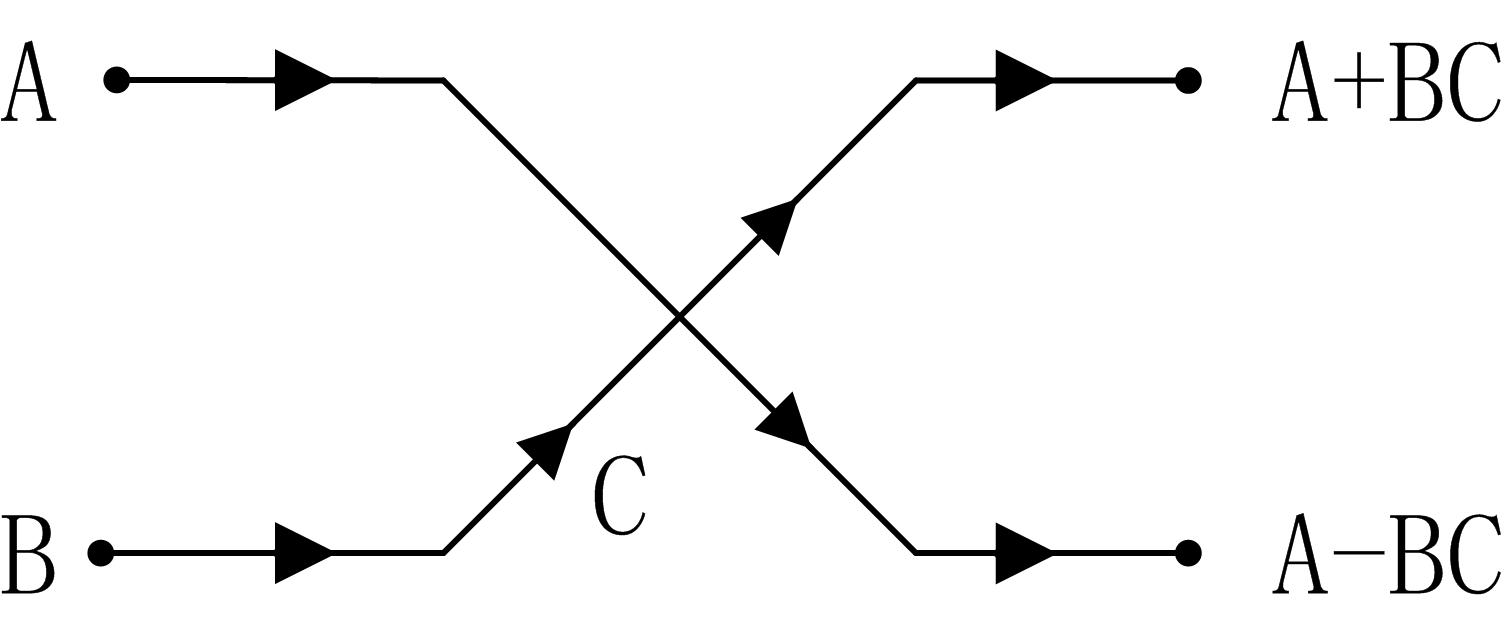
\includegraphics[width=0.50\textwidth]{diexingyunsuan.jpg}
  %\caption{蝶形运算符号}
  %\label{}
\end{figure}
显然,一个蝶形运算,需要1次复数乘法,2次复数加法。
\end{frame}
%%%%%%%%%%%%%%%%%%%%%%%%%%%%%%%%%%%%%%%%%%%%%%%%%%%%%%%%%%%%%%%%%%%%%%%%%%%%%%%%%%%%%%%%%%%%%%%%%%%%%%%%%%%%%%%%%%%%%%%%%%
%%
%%
%%
%%%%%%%%%%%%%%%%%%%%%%%%%%%%%%%%%%%%%%%%%%%%%%%%%%%%%%%%%%%%%%%%%%%%%%%%%%%%%%%%%%%%%%%%%%%%%%%%%%%%%%%%%%%%%%%%%%%%%%%%%%
\begin{frame}[shrink]\frametitle{以8点DFT为例}
\par 令$k=0$,则有
\begin{equation*} \label{eq:1}
\left\{ \begin{aligned}
         X(0) &= X_{1}(0)+  W_{N}^{0}X_{2}(0)\\
         X(4) &= X_{1}(0)-  W_{N}^{0}X_{2}(0)
\end{aligned} \right.
\end{equation*}
\par 令$k=1$,则有
\begin{equation*} \label{eq:1}
\left\{ \begin{aligned}
         X(1) &= X_{1}(1)+  W_{N}^{1}X_{2}(1)\\
         X(5) &= X_{1}(1)-  W_{N}^{1}X_{2}(1)
\end{aligned} \right.
\end{equation*}
\par 令$k=2$,则有
\begin{equation*} \label{eq:1}
\left\{ \begin{aligned}
         X(2) &= X_{1}(2)+  W_{N}^{1}X_{2}(2)\\
         X(6) &= X_{1}(2)-  W_{N}^{1}X_{2}(2)
\end{aligned} \right.
\end{equation*}
\par 令$k=3$,则有
\begin{equation*} \label{eq:1}
\left\{ \begin{aligned}
         X(3) &= X_{1}(3)+  W_{N}^{1}X_{2}(3)\\
         X(7) &= X_{1}(3)-  W_{N}^{1}X_{2}(3)
\end{aligned} \right.
\end{equation*}
\end{frame}
%%%%%%%%%%%%%%%%%%%%%%%%%%%%%%%%%%%%%%%%%%%%%%%%%%%%%%%%%%%%%%%%%%%%%%%%%%%%%%%%%%%%%%%%%%%%%%%%%%%%%%%%%%%%%%%%%%%%%%%%%%
%%
%%
%%
%%%%%%%%%%%%%%%%%%%%%%%%%%%%%%%%%%%%%%%%%%%%%%%%%%%%%%%%%%%%%%%%%%%%%%%%%%%%%%%%%%%%%%%%%%%%%%%%%%%%%%%%%%%%%%%%%%%%%%%%%%
%\begin{frame}[shrink]\frametitle{蝶形运算}
%\begin{equation*}
%\left\{ \begin{aligned}
%          X(k)\quad &=X_{1}(k) + W_{N}^{k}X_{2}(k)\\
%         X(k+\frac{N}{2})&=X_{1}(k) - W_{N}^{k}X_{2}(k)
%\end{aligned} \right.
%\end{equation*}
%这种计算方式可定义为蝶形运算。
%\begin{figure}[h]
%  \centering
%  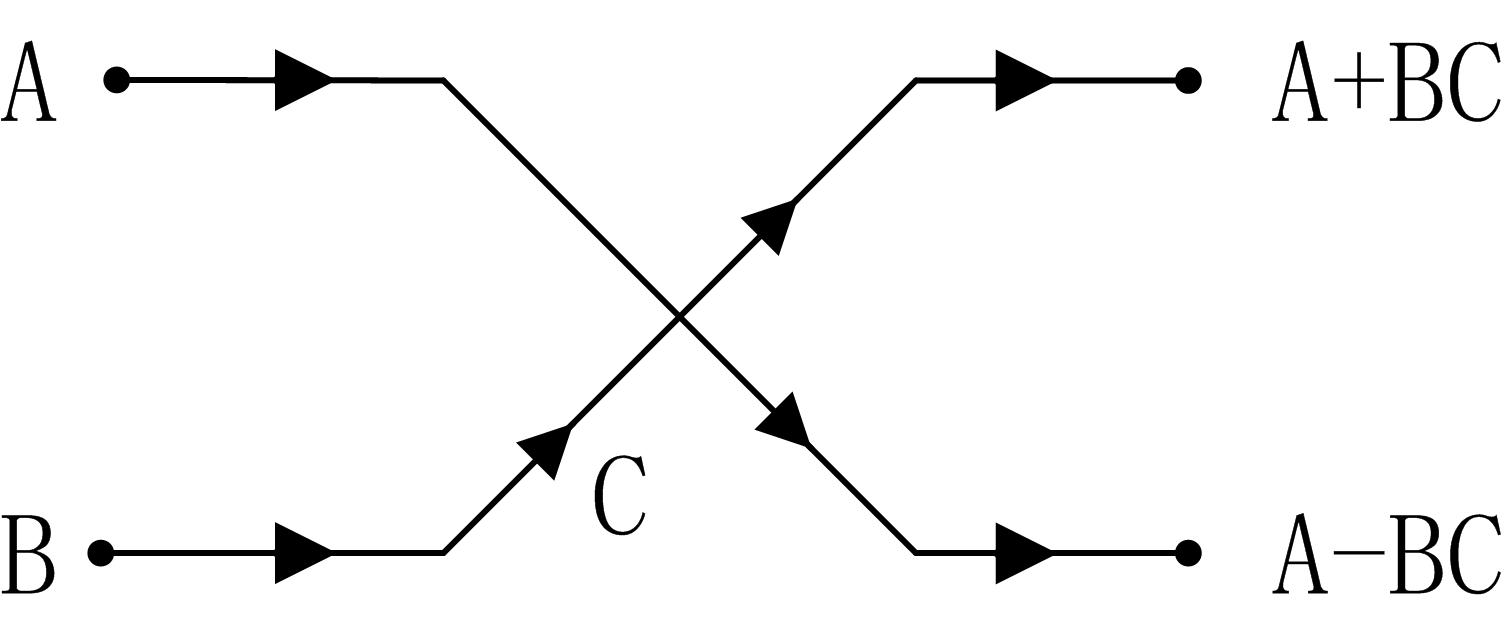
\includegraphics[width=0.50\textwidth]{diexingyunsuan.jpg}
%  %\caption{蝶形运算符号}
%  %\label{}
%\end{figure}
%\par 显然,完成\textbf{一个蝶形运算,需要一次复数乘法,两次复数加法}。
%\end{frame}
%%%%%%%%%%%%%%%%%%%%%%%%%%%%%%%%%%%%%%%%%%%%%%%%%%%%%%%%%%%%%%%%%%%%%%%%%%%%%%%%%%%%%%%%%%%%%%%%%%%%%%%%%%%%%%%%%%%%%%%%%%
%%
%%
%%
%%%%%%%%%%%%%%%%%%%%%%%%%%%%%%%%%%%%%%%%%%%%%%%%%%%%%%%%%%%%%%%%%%%%%%%%%%%%%%%%%%%%%%%%%%%%%%%%%%%%%%%%%%%%%%%%%%%%%%%%%%
\begin{frame}[shrink]\frametitle{8点DFT一次时域抽取分解运算流图}
\begin{figure}[h]
  \centering
  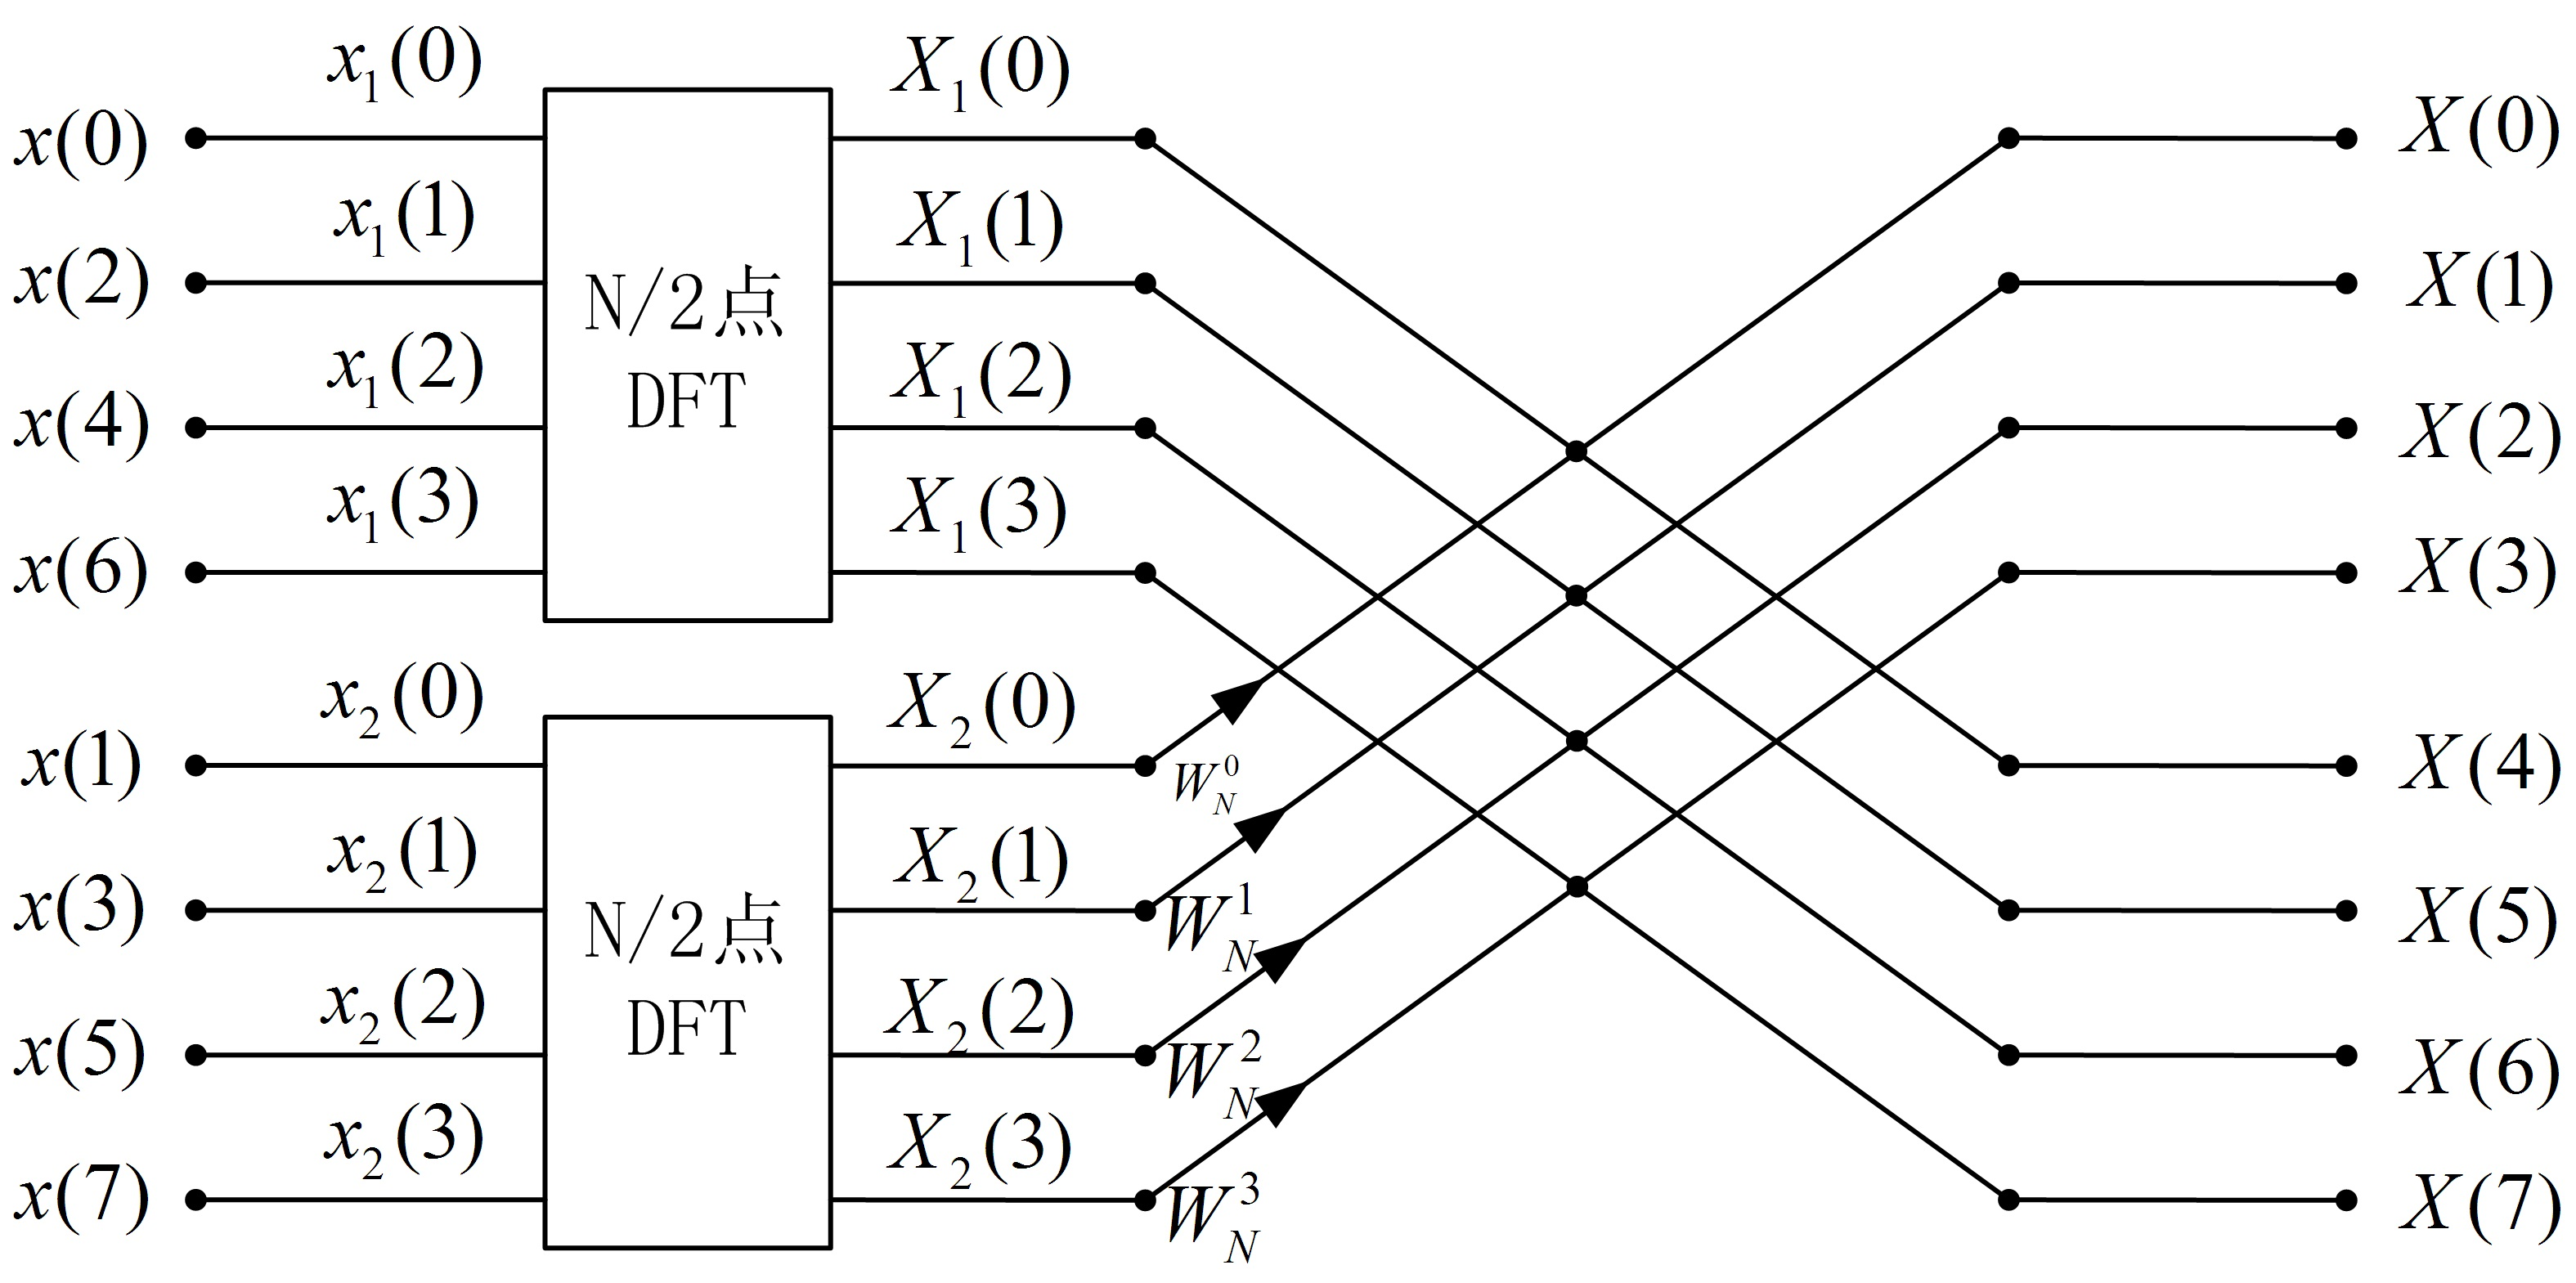
\includegraphics[width=0.99\textwidth]{8dftFirst.jpg}
  %\caption{8点DFT一次时域分解运算流图}
  %\label{}
\end{figure}
\par 一个N点DFT $\quad\Longleftrightarrow\quad$ 两个$\frac{N}{2}$点DFT+$\frac{N}{2}$次蝶形运算
%计算量分析:
%\begin{itemize}
%  \item 两个短序列:$\quad\quad\quad(\frac{N}{2})^{2}\times2=\frac{N^{2}}{2}$
%  \item N/2个蝶形:N/2个乘法
%  \item 总乘法次数,$\frac{N^{2}}{2}+\frac{N}{2}\approx \frac{N^{2}}{2}$
%\end{itemize}
\end{frame}


%%%%---------------------------------------------------------------------------------------------------
\begin{frame}[shrink]\frametitle{第一次分解后FFT计算量分析}
\begin{figure}[h]
  \centering
  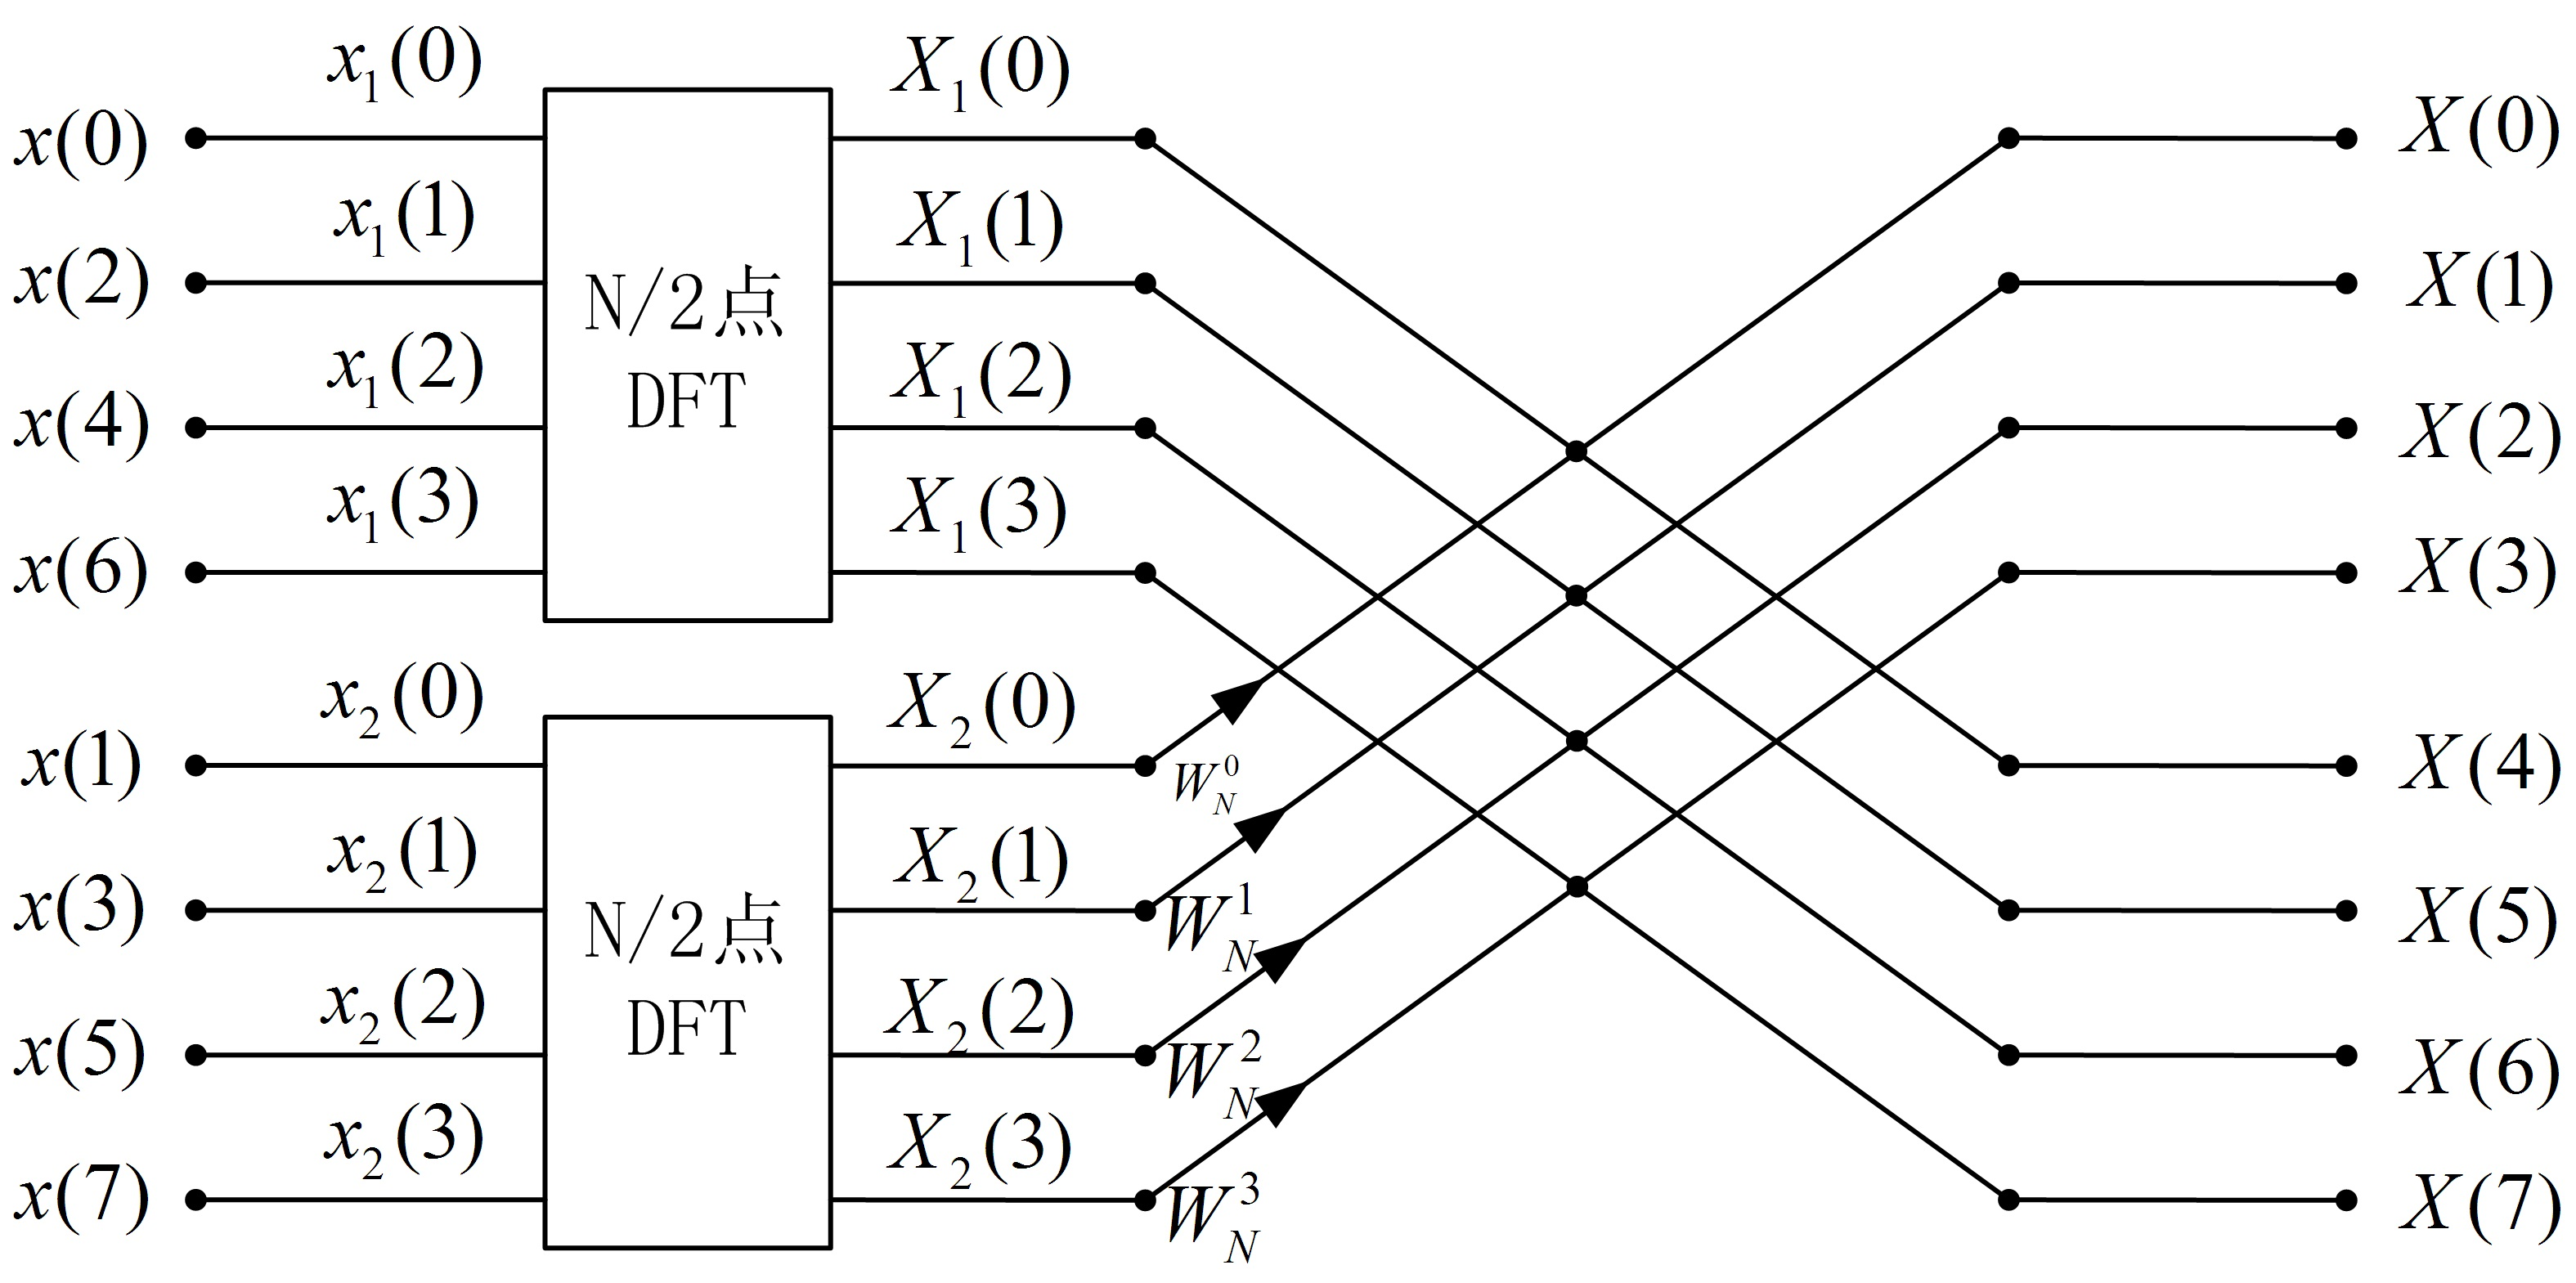
\includegraphics[width=0.5\textwidth]{8dftFirst.jpg}
\end{figure}
\par
\begin{center}
一个N点DFT $\quad\Longleftrightarrow\quad$ 两个$\frac{N}{2}$点DFT+$\frac{N}{2}$次蝶形运算
\end{center}
\par 计算量分析:
\begin{itemize}
  \item 两个短序列:$\quad\quad\quad(\frac{N}{2})^{2}\times2=\frac{N^{2}}{2}$
  \item N/2个蝶形:\quad\quad\quad N/2个乘法
  \item 总乘法次数,$\quad\quad\quad\frac{N^{2}}{2}+\frac{N}{2}\approx \frac{N^{2}}{2}$
\end{itemize}
可见,一次分解后,计算量减半。
\end{frame}
%%%%%%%%%%%%%%%%%%%%%%%%%%%%%%%%%%%%%%%%%%%%%%%%%%%%%%%%%%%%%%%%%%%%%%%%%%%%%%%%%%%%%%%%%%%%%%%%%%%%%%%%%%%%%%%%%%%%%%%%%%
%%
%%
%%
%%%%%%%%%%%%%%%%%%%%%%%%%%%%%%%%%%%%%%%%%%%%%%%%%%%%%%%%%%%%%%%%%%%%%%%%%%%%%%%%%%%%%%%%%%%%%%%%%%%%%%%%%%%%%%%%%%%%%%%%%%
\begin{frame}[shrink]\frametitle{(二)第二次分解}%\qquad $x_{1}(r)\longleftrightarrow X_{1}(k)$
经过第一次分解,将$x(n) = \{x(0),x(1),x(2),x(3),x(4),x(5),x(6),x(7)\}$分解为两个长度为$\frac{N}{2}$的短序列。

\begin{equation*}
\left\{ \begin{aligned}
    x_{1}(r) &= \{x(0),x(2),x(4),x(6)\}=x(2r)\\
    x_{2}(r) &= \{x(1),x(3),x(5),x(7)\}=x(2r+1)\\
\end{aligned} \right.
\end{equation*}
$$\mbox{设}\quad x_{1}(r)\longleftrightarrow X_{1}(k)\qquad\mbox{长}\frac{N}{2}$$
\par 再次对$x_{1}(r)$按奇偶分为两个N/4点的子序列$x_{3}(l)$、$x_{4}(l)$,即
$$
\left\{ \begin{aligned}
    x_3(l) &= x_{1}(2l)\quad\quad\quad(0\leq l\leq\frac{N}{4}-1) \\
    x_4(l) &= x_{1}(2l+1)\\
\end{aligned} \right.
$$

\end{frame}
%%%%%%%%%%%%%%%%%%%%%%%%%%%%%%%%%%%%%%%%%%%%%%%%%%%%%%%%%%%%%%%%%%%%%%%%%%%%%%%%%%%%%%%%%%%%%%%%%%%%%%%%%%%%%%%%%%%%%%%%%%
%%
%%
%%
%%%%%%%%%%%%%%%%%%%%%%%%%%%%%%%%%%%%%%%%%%%%%%%%%%%%%%%%%%%%%%%%%%%%%%%%%%%%%%%%%%%%%%%%%%%%%%%%%%%%%%%%%%%%%%%%%%%%%%%%%%
\begin{frame}[shrink]\frametitle{第二次分解——推导}
显然,对于8点DFT,此处有
$$ \label{eq:2}
\left\{ \begin{aligned}
    x_3(l) &= \{x(0),x(4)\}\quad\quad\quad\quad\quad\quad\quad\quad\quad\\
    x_4(l) &= \{x(2),x(6)\}\\
\end{aligned} \right.
$$
如果
$$
\left\{ \begin{aligned}
    x_3(l) &\longleftrightarrow X_3(k)\quad\quad\quad(0\leq l\leq\frac{N}{4}-1)\\
    x_4(l) &\longleftrightarrow X_4(k)\\
\end{aligned} \right.
$$
\par 可将$X_1(k)$用$X_3(k),X_4(k)$表示。\newline
与前述类似,可类推下列公式。
%\begin{itemize}
%  \item \quad\quad$X_1(k)=X_{3}(k) + W_{\frac{N}{2}}^{k}X_{4}(k)$
%  \item $X_1(k+\frac{N}{4})=X_{3}(k) - W_{\frac{N}{2}}^{k}X_{4}(k)$
%\end{itemize}
$$
\left\{ \begin{aligned}
     X_1(k)\quad      &=  X_{3}(k) + W_{\frac{N}{2}}^{k}X_{4}(k)   \quad\quad(0\leq k\leq\frac{N}{4}-1)\\
    X_1(k+\frac{N}{4}) &=  X_{3}(k) - W_{\frac{N}{2}}^{k}X_{4}(k)\\
\end{aligned} \right.
$$
%\par 前一半:\quad\quad$X_1(k)=X_{3}(k) + W_{\frac{N}{2}}^{k}X_{4}(k)$
%\par 后一半:$X_1(k+\frac{N}{4})=X_{3}(k) - W_{\frac{N}{2}}^{k}X_{4}(k)$
\end{frame}
%%%%%%%%%%%%%%%%%%%%%%%%%%%%%%%%%%%%%%%%%%%%%%%%%%%%%%%%%%%%%%%%%%%%%%%%%%%%%%%%%%%%%%%%%%%%%%%%%%%%%%%%%%%%%%%%%%%%%%%%%%
%%
%%
%%
%%%%%%%%%%%%%%%%%%%%%%%%%%%%%%%%%%%%%%%%%%%%%%%%%%%%%%%%%%%%%%%%%%%%%%%%%%%%%%%%%%%%%%%%%%%%%%%%%%%%%%%%%%%%%%%%%%%%%%%%%%
\begin{frame}[shrink]\frametitle{第二次分解——示例}
%\par 已知$X_3(k),X_4(k)$,求$X_1(k)$,可类推前面公式。
%\par 前一半:\quad\quad$X_1(k)=X_{3}(k) + W_{\frac{N}{2}}^{k}X_{4}(k)$
%\par 后一半:$X_1(k+\frac{N}{4})=X_{3}(k) - W_{\frac{N}{2}}^{k}X_{4}(k)$
例如:
\par 令$k=0$,则有
\begin{equation*} \label{eq:1}
\left\{ \begin{aligned}
         X_1(0) &= X_{3}(0)+  W_{\frac{N}{2}}^{0}X_{4}(0)\\
         X_1(2) &= X_{3}(0)-  W_{\frac{N}{2}}^{0}X_{4}(0)
\end{aligned} \right.
\end{equation*}
\par 令$k=1$,则有
\begin{equation*} \label{eq:1}
\left\{ \begin{aligned}
         X_1(1) &= X_{3}(1)+  W_{\frac{N}{2}}^{1}X_{4}(1)\\
         X_1(3) &= X_{3}(1)-  W_{\frac{N}{2}}^{1}X_{4}(1)
\end{aligned} \right.
\end{equation*}

\end{frame}
%%%%%%%%%%%%%%%%%%%%%%%%%%%%%%%%%%%%%%%%%%%%%%%%%%%%%%%%%%%%%%%%%%%%%%%%%%%%%%%%%%%%%%%%%%%%%%%%%%%%%%%%%%%%%%%%%%%%%%%%%%
%%
%%
%%
%%%%%%%%%%%%%%%%%%%%%%%%%%%%%%%%%%%%%%%%%%%%%%%%%%%%%%%%%%%%%%%%%%%%%%%%%%%%%%%%%%%%%%%%%%%%%%%%%%%%%%%%%%%%%%%%%%%%%%%%%%
\begin{frame}[shrink]\frametitle{8点DFT二次时域抽取分解运算流图}
\begin{figure}[h]
  \centering
  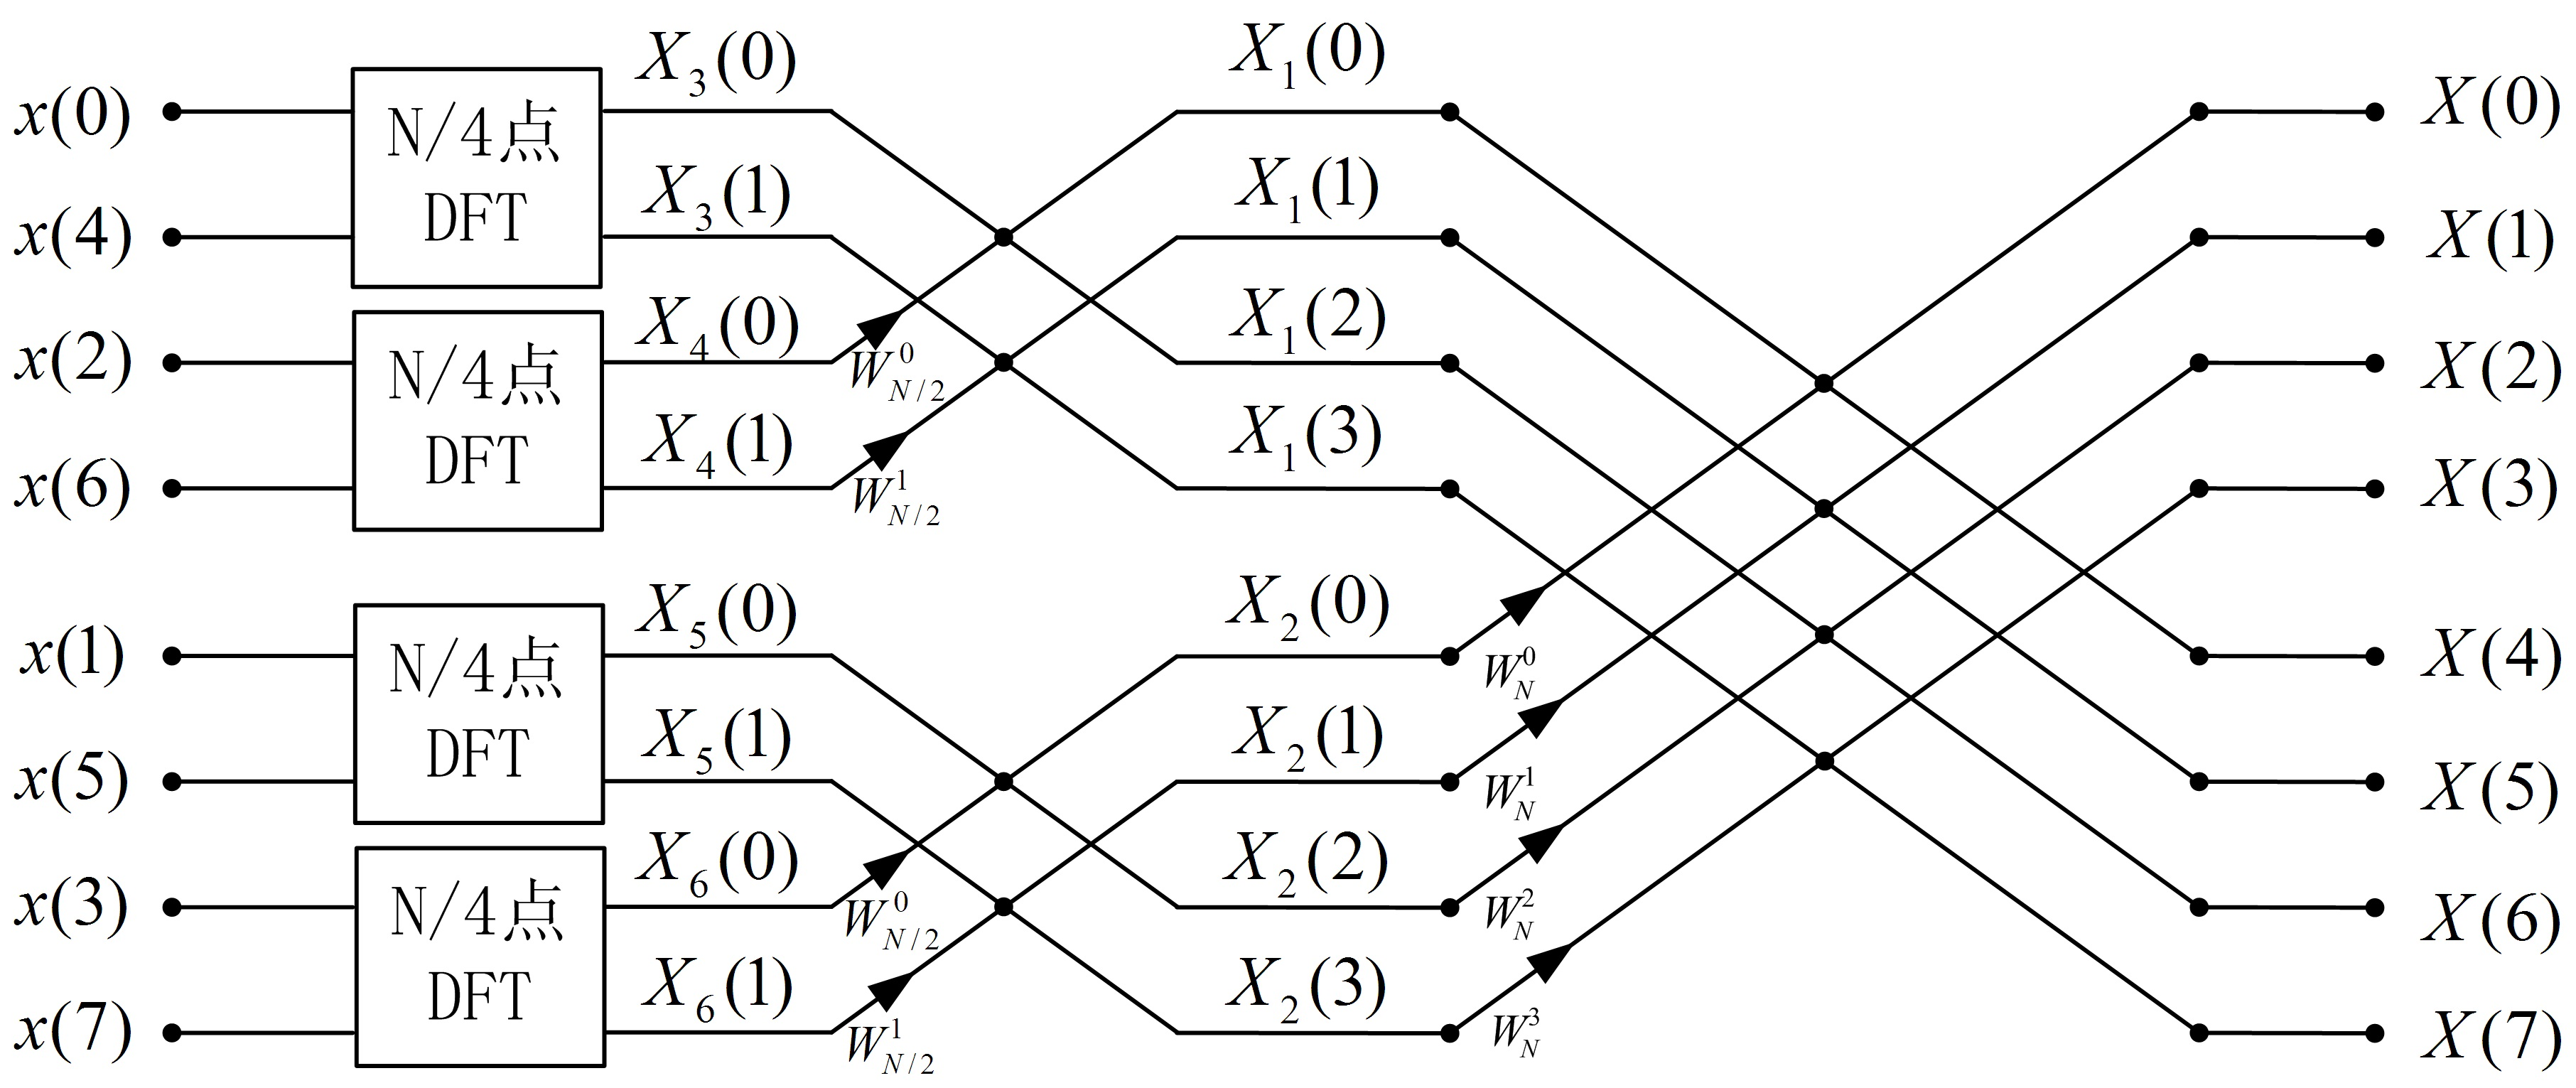
\includegraphics[width=1\textwidth]{8dftSecond.jpg}
  %\caption{8点DFT一次时域分解运算流图}
  %\label{}
\end{figure}
\end{frame}
%%%%%%%%%%%%%%%%%%%%%%%%%%%%%%%%%%%%%%%%%%%%%%%%%%%%%%%%%%%%%%%%%%%%%%%%%%%%%%%%%%%%%%%%%%%%%%%%%%%%%%%%%%%%%%%%%%%%%%%%%%
%%
%%
%%
%%%%%%%%%%%%%%%%%%%%%%%%%%%%%%%%%%%%%%%%%%%%%%%%%%%%%%%%%%%%%%%%%%%%%%%%%%%%%%%%%%%%%%%%%%%%%%%%%%%%%%%%%%%%%%%%%%%%%%%%%%
\begin{frame}[shrink]\frametitle{最后一次分解}
一直分解到短序列长度为2,不能再分。此时,DFT计算按定义来算。
\par \textbf{例如:}当N=2时,
\begin{equation*}
\begin{split}
X(k)&= \sum_{n=0}^{1}x(n)W_{2}^{kn} \quad\quad(0\leq k\leq1)\\
    &=x(0)W_{2}^{0} + x(1)W_{2}^{k}\\
    &=x(0) + x(1)W_{2}^{k}\quad\quad(0\leq k\leq1)
\end{split}
\end{equation*}
将$k=0$,$k=1$代入可的:
\begin{equation*} \label{eq:2}
\left\{ \begin{aligned}
  X(0) &= x(0) +x(1)\\
  X(1) &= x(0) -x(1) \quad\quad\quad( W_2^1=-1)
\end{aligned} \right.
\end{equation*}
%此时DFT的计算非常简单。
\end{frame}
%%%%%%%%%%%%%%%%%%%%%%%%%%%%%%%%%%%%%%%%%%%%%%%%%%%%%%%%%%%%%%%%%%%%%%%%%%%%%%%%%%%%%%%%%%%%%%%%%%%%%%%%%%%%%%%%%%%%%%%%%%
%%
%%
%%
%%%%%%%%%%%%%%%%%%%%%%%%%%%%%%%%%%%%%%%%%%%%%%%%%%%%%%%%%%%%%%%%%%%%%%%%%%%%%%%%%%%%%%%%%%%%%%%%%%%%%%%%%%%%%%%%%%%%%%%%%%
\begin{frame}[shrink]\frametitle{8点DFT第三次时域分解运算流图}
\begin{figure}[h]
  \centering
  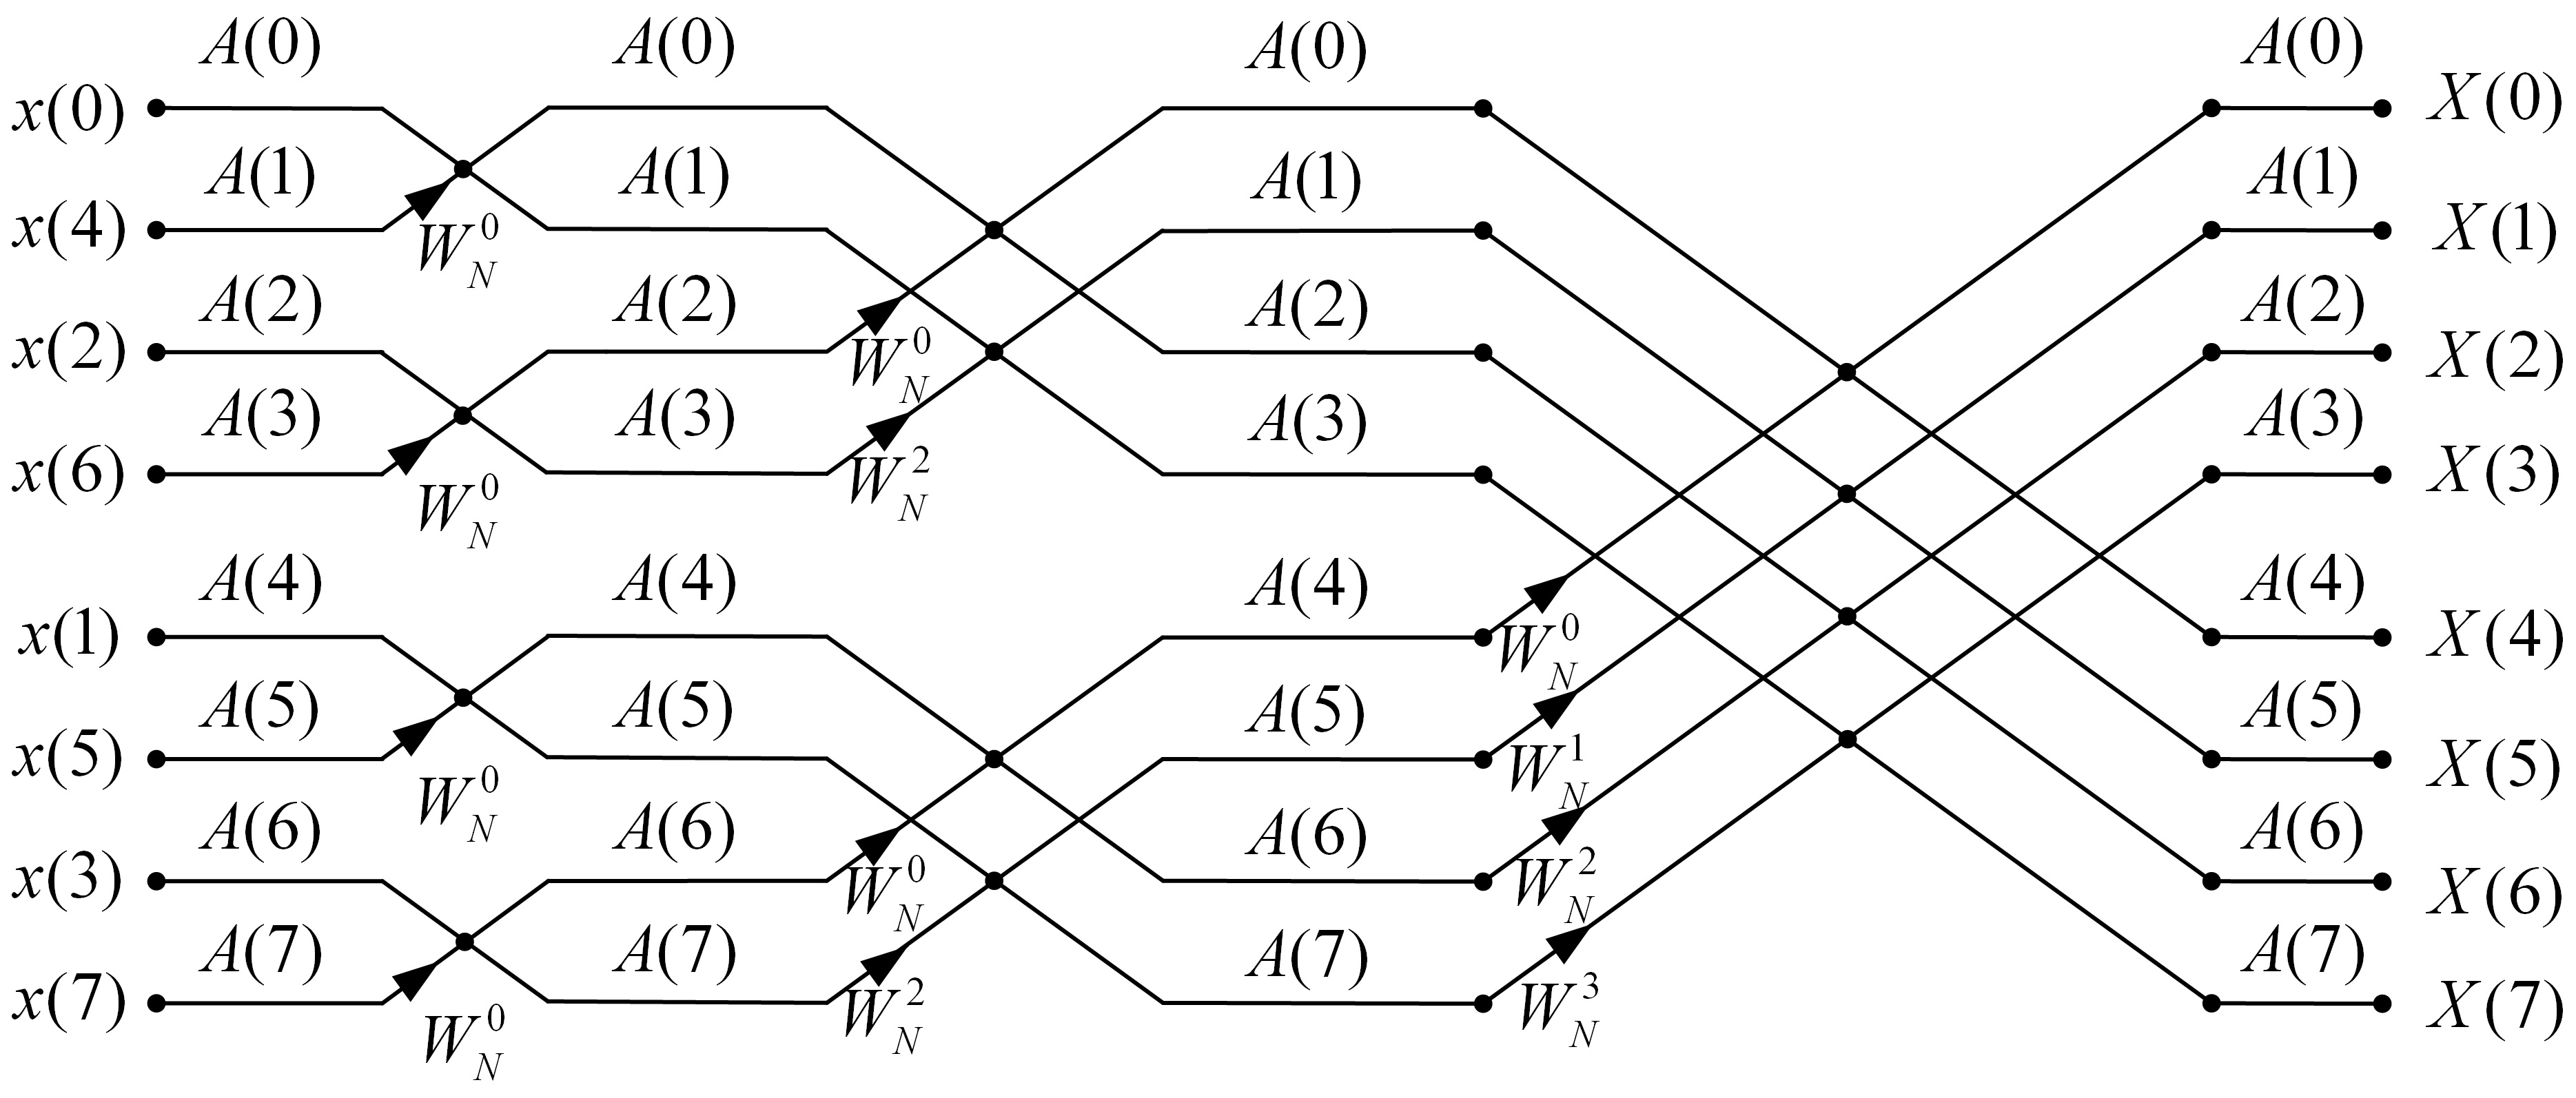
\includegraphics[width=0.99\textwidth]{8dftThird.jpg}
  %\caption{8点DFT一次时域分解运算流图}
  %\label{}
\end{figure}
\end{frame}
%%%%%%%%%%%%%%%%%%%%%%%%%%%%%%%%%%%%%%%%%%%%%%%%%%%%%%%%%%%%%%%%%%%%%%%%%%%%%%%%%%%%%%%%%%%%%%%%%%%%%%%%%%%%%%%%%%%%%%%%%%
%%
%%
%%
%%%%%%%%%%%%%%%%%%%%%%%%%%%%%%%%%%%%%%%%%%%%%%%%%%%%%%%%%%%%%%%%%%%%%%%%%%%%%%%%%%%%%%%%%%%%%%%%%%%%%%%%%%%%%%%%%%%%%%%%%%
\subsection{DIT-FFT算法计算量}
%%%%%%%%%%%%%%%%%%%%%%%%%%%%%%%%%%%%%%%%%%%%%%%%%%%%%%%%%%%%%%%%%%%%%%%%%%%%%%%%%%%%%%%%%%%%%%%%%%%%%%%%%%%%%%%%%%%%%%%%%%
%%
%%
%%
%%%%%%%%%%%%%%%%%%%%%%%%%%%%%%%%%%%%%%%%%%%%%%%%%%%%%%%%%%%%%%%%%%%%%%%%%%%%%%%%%%%%%%%%%%%%%%%%%%%%%%%%%%%%%%%%%%%%%%%%%%
\begin{frame}[shrink]\frametitle{DIT-FFT算法计算量分析}
设$N=2^M\quad(M=log_2 N)$,
\begin{enumerate}
  \item [1] 运算流图应有$M$级蝶形。
  \item [2] 每一级都由$\frac{N}{2}$个蝶形构成,
  \item [3] 每个蝶形需要一次复数乘法,两次复数加法,
\end{enumerate}
因此,M级蝶形运算总的复数乘法次数为:$M\cdot\frac{N}{2}=\frac{N}{2}log_2 N$

以乘法为例:
$$\frac{DFT}{FFT}= \frac{N^2}{\frac{N}{2}log_2 N}=\frac{2N}{log_2 N}$$
\begin{itemize}
  \item 当$N=2^{10}=1024$时,$\frac{DFT}{FFT}=204.8$
  \item 当$N=2^{20}=1024x1024$时,$\frac{DFT}{FFT}= 104857.6$
\end{itemize}
可见,N越大,节约的时间越多。
\end{frame}
%%%%%%%%%%%%%%%%%%%%%%%%%%%%%%%%%%%%%%%%%%%%%%%%%%%%%%%%%%%%%%%%%%%%%%%%%%%%%%%%%%%%%%%%%%%%%%%%%%%%%%%%%%%%%%%%%%%%%%%%%%
%%
%%
%%
%%%%%%%%%%%%%%%%%%%%%%%%%%%%%%%%%%%%%%%%%%%%%%%%%%%%%%%%%%%%%%%%%%%%%%%%%%%%%%%%%%%%%%%%%%%%%%%%%%%%%%%%%%%%%%%%%%%%%%%%%%
\section{DIT-FFT的运算规律与编程思想}
\subsection{原位计算(同址计算)}
%%%%%%%%%%%%%%%%%%%%%%%%%%%%%%%%%%%%%%%%%%%%%%%%%%%%%%%%%%%%%%%%%%%%%%%%%%%%%%%%%%%%%%%%%%%%%%%%%%%%%%%%%%%%%%%%%%%%%%%%%%
%%
%%
%%
%%%%%%%%%%%%%%%%%%%%%%%%%%%%%%%%%%%%%%%%%%%%%%%%%%%%%%%%%%%%%%%%%%%%%%%%%%%%%%%%%%%%%%%%%%%%%%%%%%%%%%%%%%%%%%%%%%%%%%%%%%
\begin{frame}[shrink]\frametitle{原位计算}

DIT-FFT的运算过程很有规律
\begin{itemize}
  \item [1] N点的FFT共进行M级运算,每级有$\frac{N}{2}$个蝶形;
  \item [2] 同一级中,每个蝶形的两个输入数据只对计算本蝶形有用;
  \item [3] 且输入输出处于同一条水平线上,这意味着计算完一个蝶形后,所输出数据可立即存入原输入数据所占用的存储单元。
\end{itemize}
\begin{figure}[h]
  \centering
  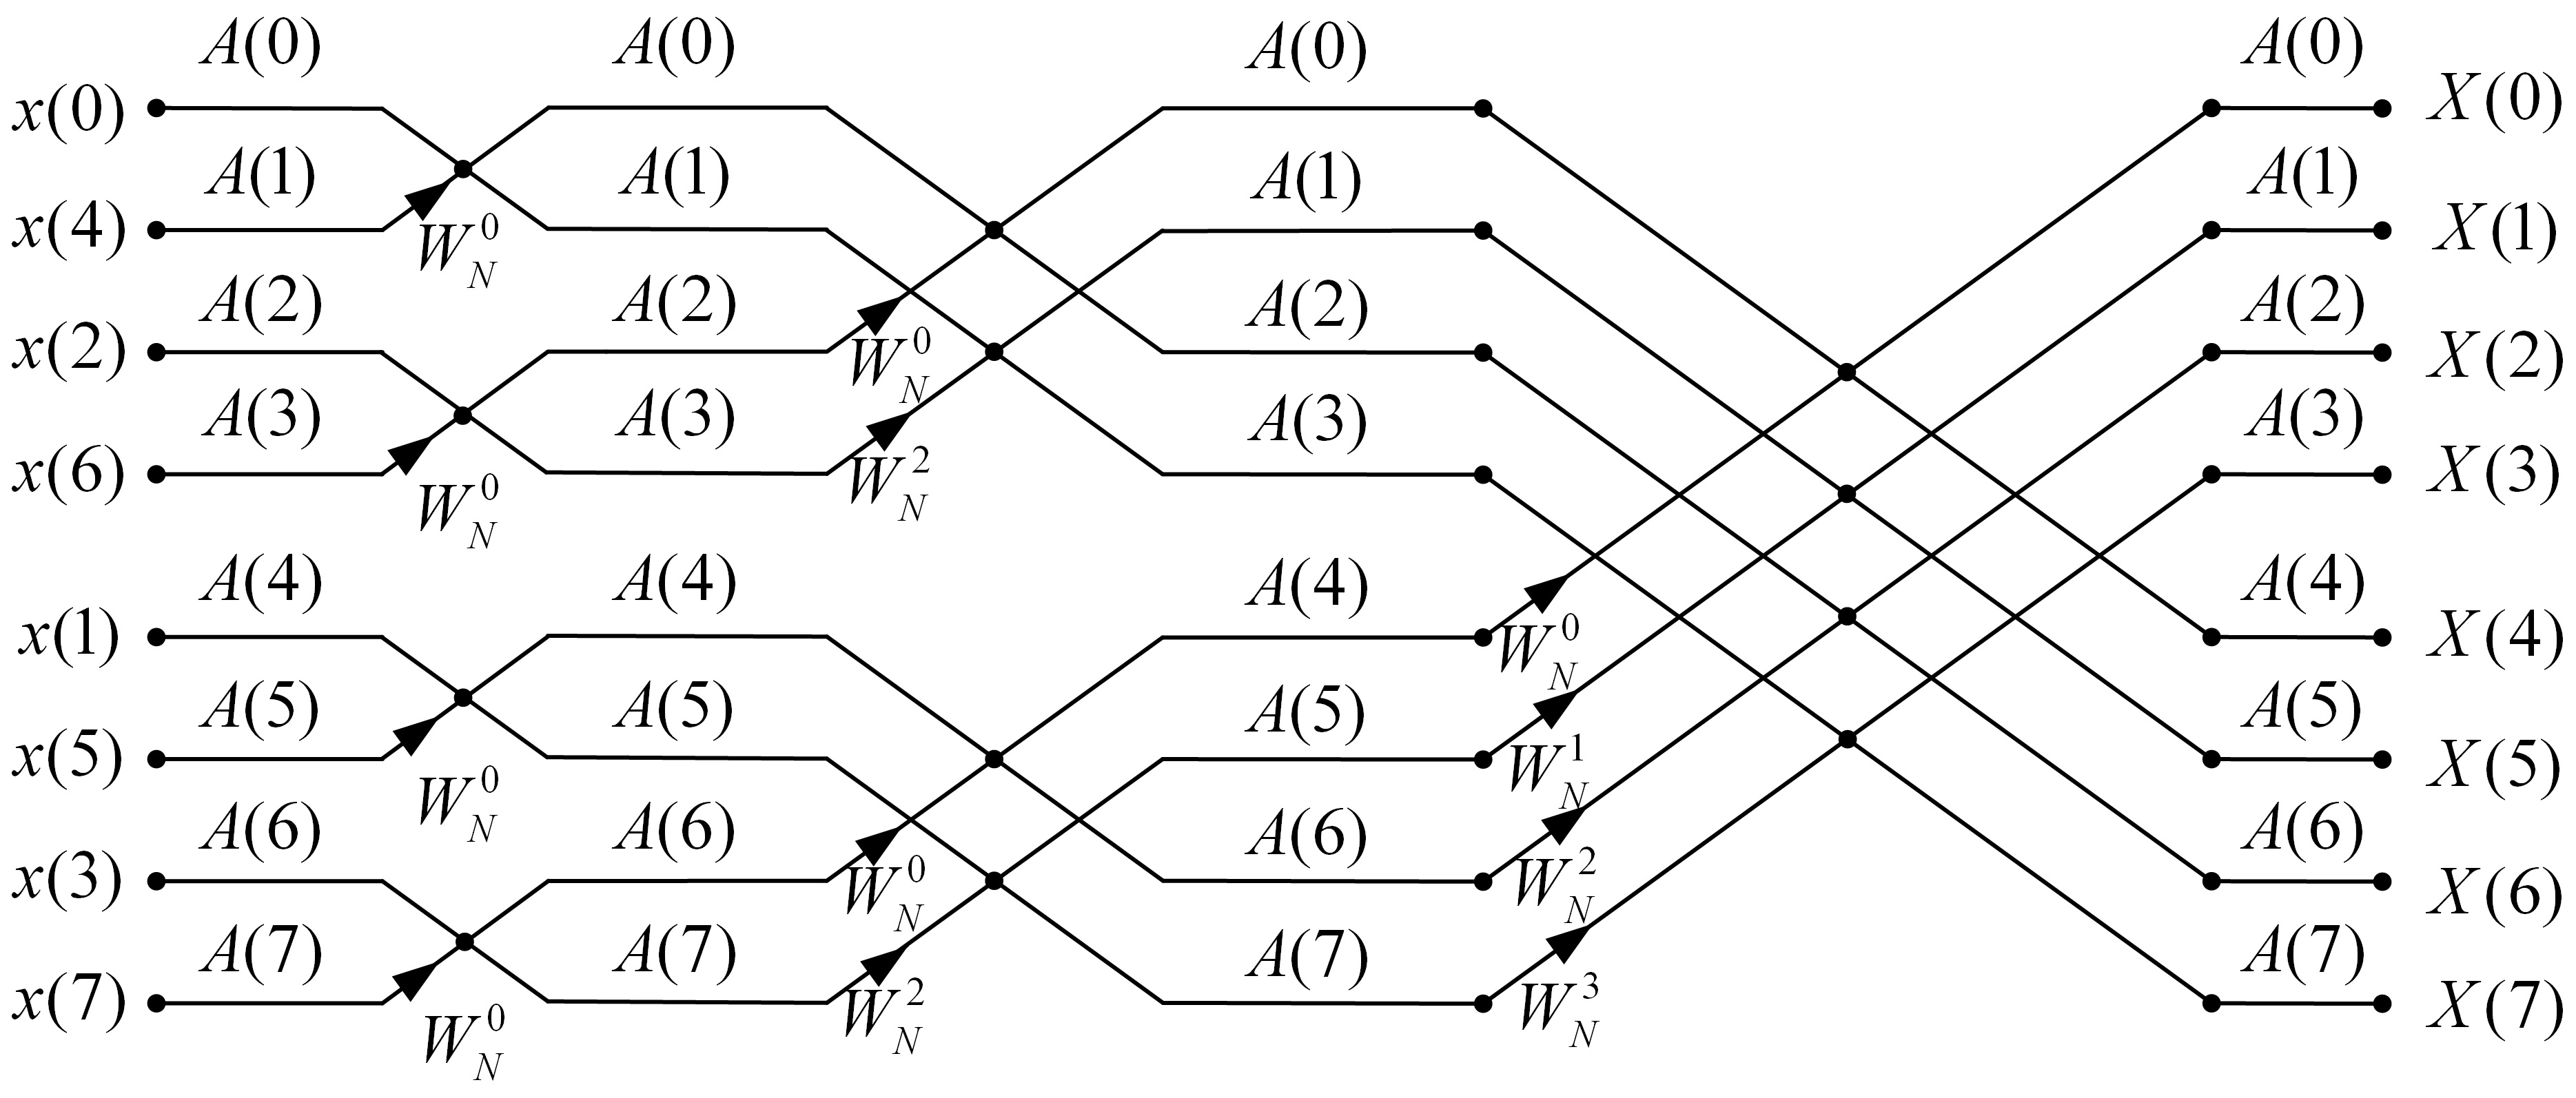
\includegraphics[width=0.75\textwidth]{8dftThird.jpg}
\end{figure}
这种利用同一存储单元存储蝶形计算输入输出的方法称为原位计算。可以节省大量内存,使设备成本降低。
\end{frame}
%%%%%%%%%%%%%%%%%%%%%%%%%%%%%%%%%%%%%%%%%%%%%%%%%%%%%%%%%%%%%%%%%%%%%%%%%%%%%%%%%%%%%%%%%%%%%%%%%%%%%%%%%%%%%%%%%%%%%%%%%
%
%
%
%%%%%%%%%%%%%%%%%%%%%%%%%%%%%%%%%%%%%%%%%%%%%%%%%%%%%%%%%%%%%%%%%%%%%%%%%%%%%%%%%%%%%%%%%%%%%%%%%%%%%%%%%%%%%%%%%%%%%%%%%%
\subsection{旋转因子$W_N^p$的变化规律}
%%%%%%%%%%%%%%%%%%%%%%%%%%%%%%%%%%%%%%%%%%%%%%%%%%%%%%%%%%%%%%%%%%%%%%%%%%%%%%%%%%%%%%%%%%%%%%%%%%%%%%%%%%%%%%%%%%%%%%%%%%
%%
%%
%%
%%%%%%%%%%%%%%%%%%%%%%%%%%%%%%%%%%%%%%%%%%%%%%%%%%%%%%%%%%%%%%%%%%%%%%%%%%%%%%%%%%%%%%%%%%%%%%%%%%%%%%%%%%%%%%%%%%%%%%%%%%
\begin{frame}[shrink]\frametitle{旋转因子}
\begin{enumerate}
  \item N点DIT-DFT运算流图中,每级都有N/2个蝶形,每个蝶形都要乘以因子$W_N^p$。
  \item 这里称$W_N^p$为旋转因子,$p$称为旋转因子的指数。
\end{enumerate}

\begin{figure}[h]
  \centering
  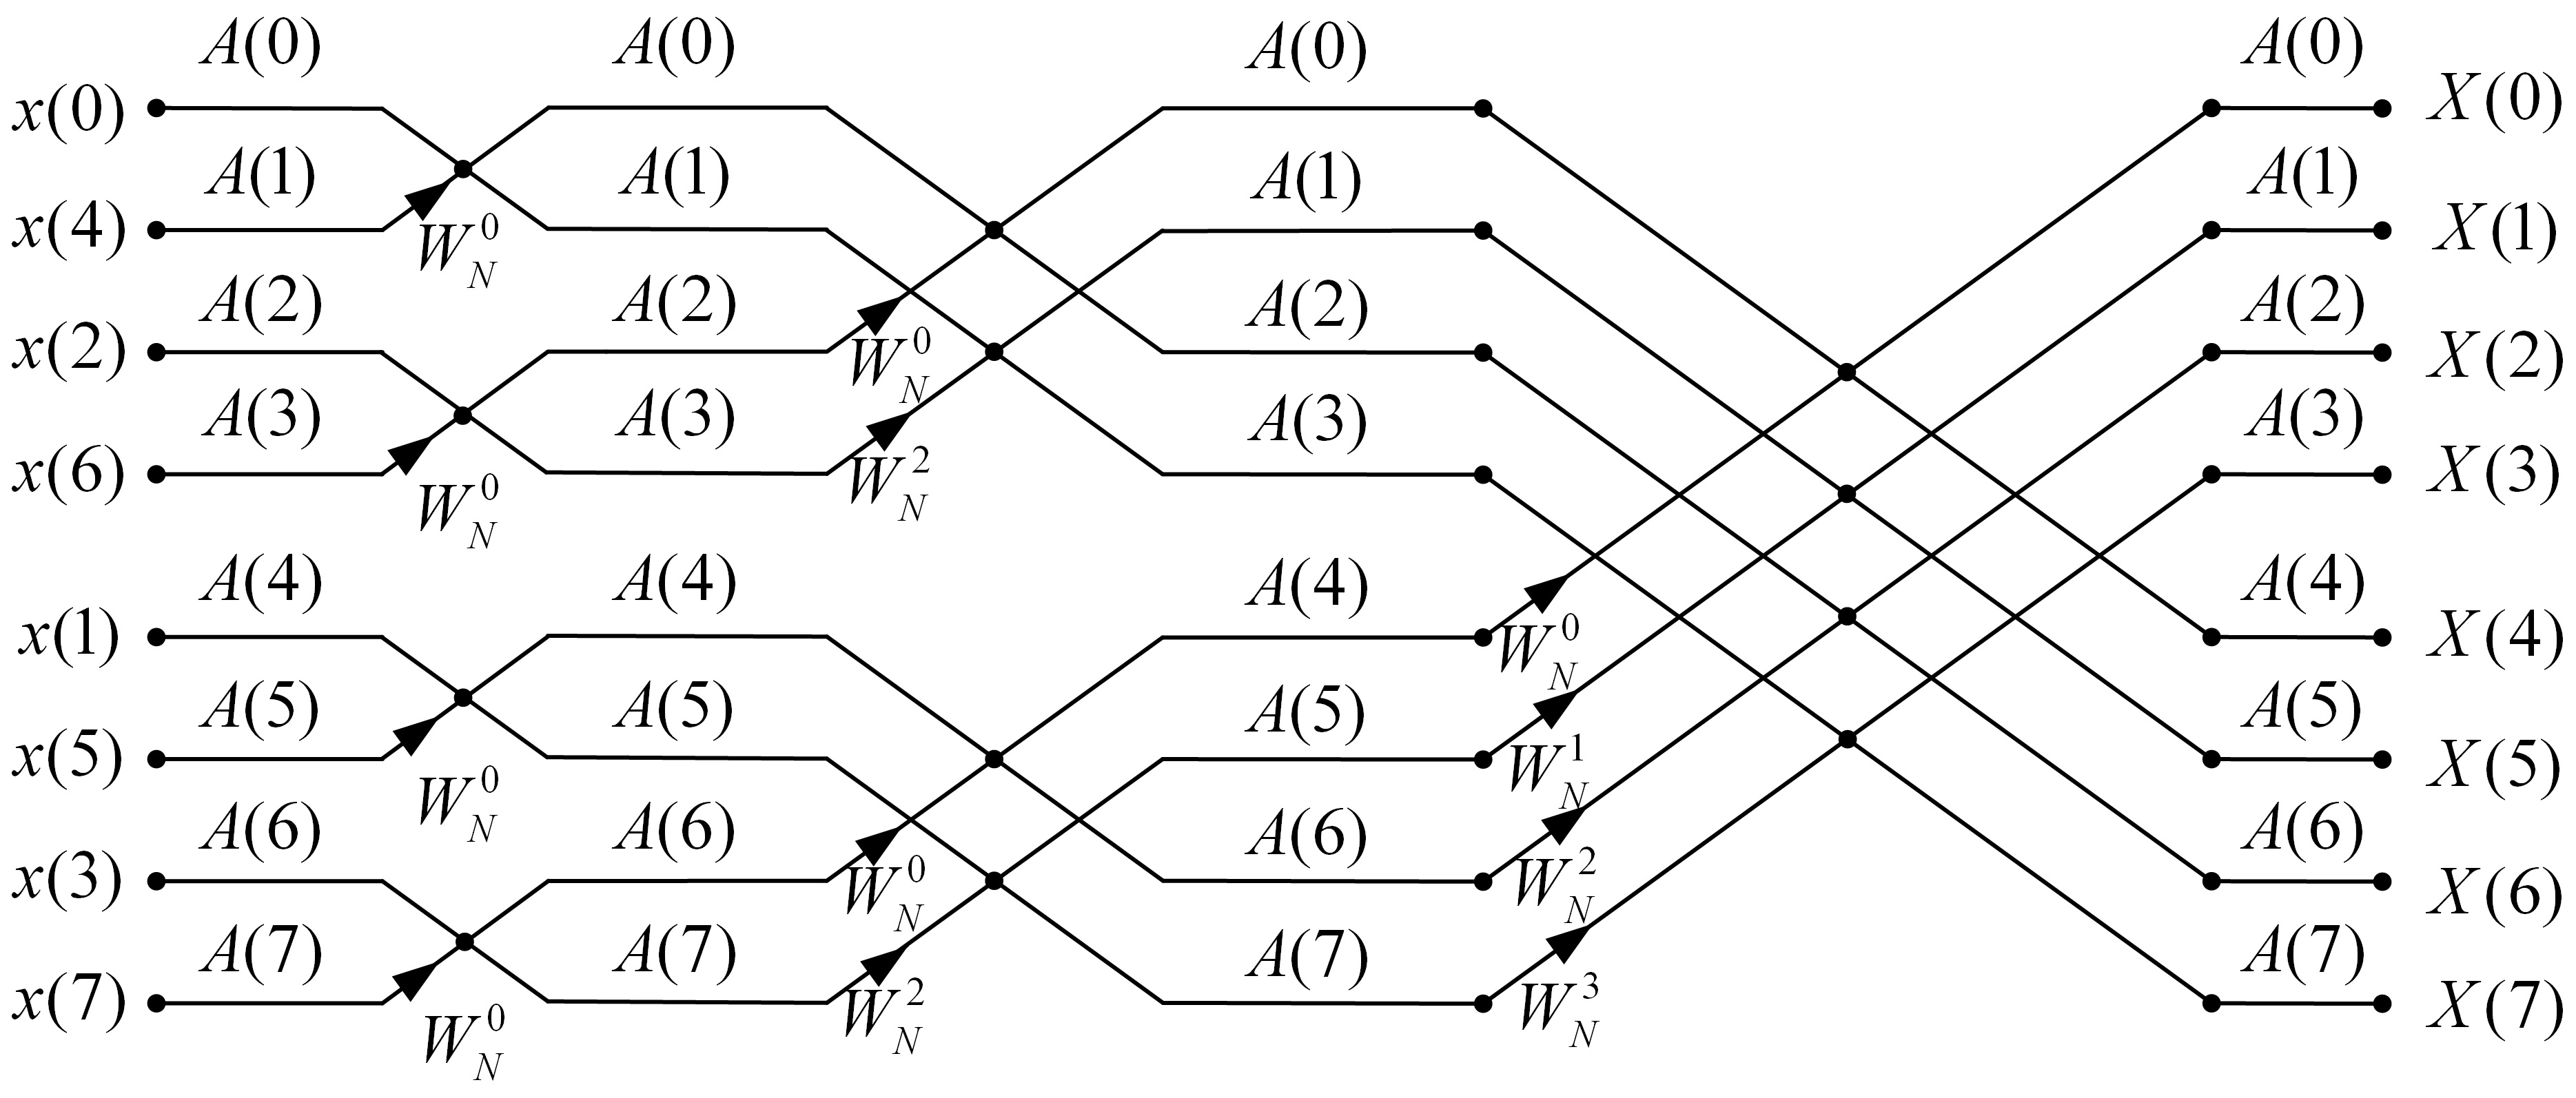
\includegraphics[width=0.99\textwidth]{8dftThird.jpg}
\end{figure}
\end{frame}
%%%%%%%%%%%%%%%%%%%%%%%%%%%%%%%%%%%%%%%%%%%%%%%%%%%%%%%%%%%%%%%%%%%%%%%%%%%%%%%%%%%%%%%%%%%%%%%%%%%%%%%%%%%%%%%%%%%%%%%%%%
%%
%%
%%
%%%%%%%%%%%%%%%%%%%%%%%%%%%%%%%%%%%%%%%%%%%%%%%%%%%%%%%%%%%%%%%%%%%%%%%%%%%%%%%%%%%%%%%%%%%%%%%%%%%%%%%%%%%%%%%%%%%%%%%%%%
\begin{frame}\frametitle{旋转因子$W_N^p$与运算级数的关系}%[allowframebreaks]
%
设L为从左到右的运算级数,即$L=1,2,3,\cdots,M$,
有以下规律:
\pause
\begin{enumerate}
  \item [1] 第$L$级一共有$2^{L-1}$个不同的旋转因子。
  \item [2] 第$L$级中,
        $$W_N^p=W_{2^L}^{J},\quad\quad\quad J=0,1,\cdots,(2^{L-1}-1)$$
        \pause 如: L=1时,$\quad W_N^p=W_2^J\quad\quad\quad J=0$
        \par 推导:
        $$W_{2^L}^{J} = W_{2^M\cdot2^{L-M}}^{J} = W_{N\cdot2^{L-M}}^{J} = W_{N}^{J/2^{L-M}} = W_{N}^{J\cdot 2^{M-L}} =W_N^p$$
        \pause 显然有:
        $$p=J\cdot 2^{M-L}$$
\end{enumerate}
\end{frame}
%%%%%%%%%%%%%%%%%%%%%%%%%%%%%%%%%%%%%%%%%%%%%%%%%%%%%%%%%%%%%%%%%%%%%%%%%%%%%%%%%%%%%%%%%%%%%%%%%%%%%%%%%%%%%%%%%%%%%%%%%
%
%
%
%%%%%%%%%%%%%%%%%%%%%%%%%%%%%%%%%%%%%%%%%%%%%%%%%%%%%%%%%%%%%%%%%%%%%%%%%%%%%%%%%%%%%%%%%%%%%%%%%%%%%%%%%%%%%%%%%%%%%%%%%
\begin{frame}[shrink]\frametitle{以N=8为例,旋转因子为:}%[allowframebreaks][shrink]
$$p=J\cdot 2^{M-L} \quad\quad\quad J=(0,1,\cdots,(2^{L-1}-1))$$
\par 例如:8点DFT时,M=3,有
\begin{enumerate}
  \item $L=1,\quad J=(0)  $%\quad\quad\quad\quad p=J\cdot 2^{M-L}=J\cdot2=(0)$
        \begin{itemize}
          \item $p=J\cdot 2^{M-L}=J\cdot 4=(0)$
          \item $\mbox{旋转因子为:}  W_{N}^{0}$
        \end{itemize}
  \item $L=2,\quad J=(0,1) $%\quad\quad\quad\quad p=J\cdot 2^{M-L}=J\cdot2=(0,2)$
        \begin{itemize}
          \item $p=J\cdot 2^{M-L}=J\cdot2=(0,2)$
          \item $\mbox{旋转因子为:}  W_{N}^{0}\quad W_{N}^{2}$
        \end{itemize}
  \item $L=3,\quad J=(0,1,2,3)$% \quad\quad p=J\cdot 2^{M-L}=J=(0,1,2,3)$
        \begin{itemize}
          \item $p=J\cdot 2^{M-L}=J=(0,1,2,3)$
          \item $\mbox{旋转因子为:}  W_{N}^{0}\quad W_{N}^{1}\quad W_{N}^{2}\quad W_{N}^{3}$
        \end{itemize}
\end{enumerate}

\end{frame}
%%%%%%%%%%%%%%%%%%%%%%%%%%%%%%%%%%%%%%%%%%%%%%%%%%%%%%%%%%%%%%%%%%%%%%%%%%%%%%%%%%%%%%%%%%%%%%%%%%%%%%%%%%%%%%%%%%%%%%%%%
%
%
%
%%%%%%%%%%%%%%%%%%%%%%%%%%%%%%%%%%%%%%%%%%%%%%%%%%%%%%%%%%%%%%%%%%%%%%%%%%%%%%%%%%%%%%%%%%%%%%%%%%%%%%%%%%%%%%%%%%%%%%%%%
\subsection{蝶形运算规律}
%%%%%%%%%%%%%%%%%%%%%%%%%%%%%%%%%%%%%%%%%%%%%%%%%%%%%%%%%%%%%%%%%%%%%%%%%%%%%%%%%%%%%%%%%%%%%%%%%%%%%%%%%%%%%%%%%%%%%%%%%%
%%
%%
%%
%%%%%%%%%%%%%%%%%%%%%%%%%%%%%%%%%%%%%%%%%%%%%%%%%%%%%%%%%%%%%%%%%%%%%%%%%%%%%%%%%%%%%%%%%%%%%%%%%%%%%%%%%%%%%%%%%%%%%%%%%%
\begin{frame}[shrink]\frametitle{蝶形运算规律}
在第L级中,有
\begin{enumerate}
  \item [1] 每个蝶形两个输入端相距点数为:$B=2^{L-1}$
%        \par $\quad\quad\quad L=1\quad\quad\quad B=1$
%        \par $\quad\quad\quad L=2\quad\quad\quad B=2$
%        \par $\quad\quad\quad L=3\quad\quad\quad B=4$
  \item [2] 有$B=2^{L-1}$个不同的旋转因子
  \item [3] 同一个旋转因子,对应相邻间隔为$2^L$点的$2^{M-L}$ 个蝶形
%        \par $\quad L=1\quad$对应$\quad2^{3-1}=4\quad$个蝶形,相距$\quad2^1=2\quad$个点。
%        \par $\quad L=2\quad$对应$\quad2^{3-2}=2\quad$个蝶形,相距$\quad2^2=4\quad$个点。
%        \par $\quad L=3\quad$对应$\quad2^{3-3}=1\quad$个蝶形,相距$\quad2^3=8$个点(意味着只有一个点)。
\end{enumerate}
\begin{figure}[h]
  \centering
  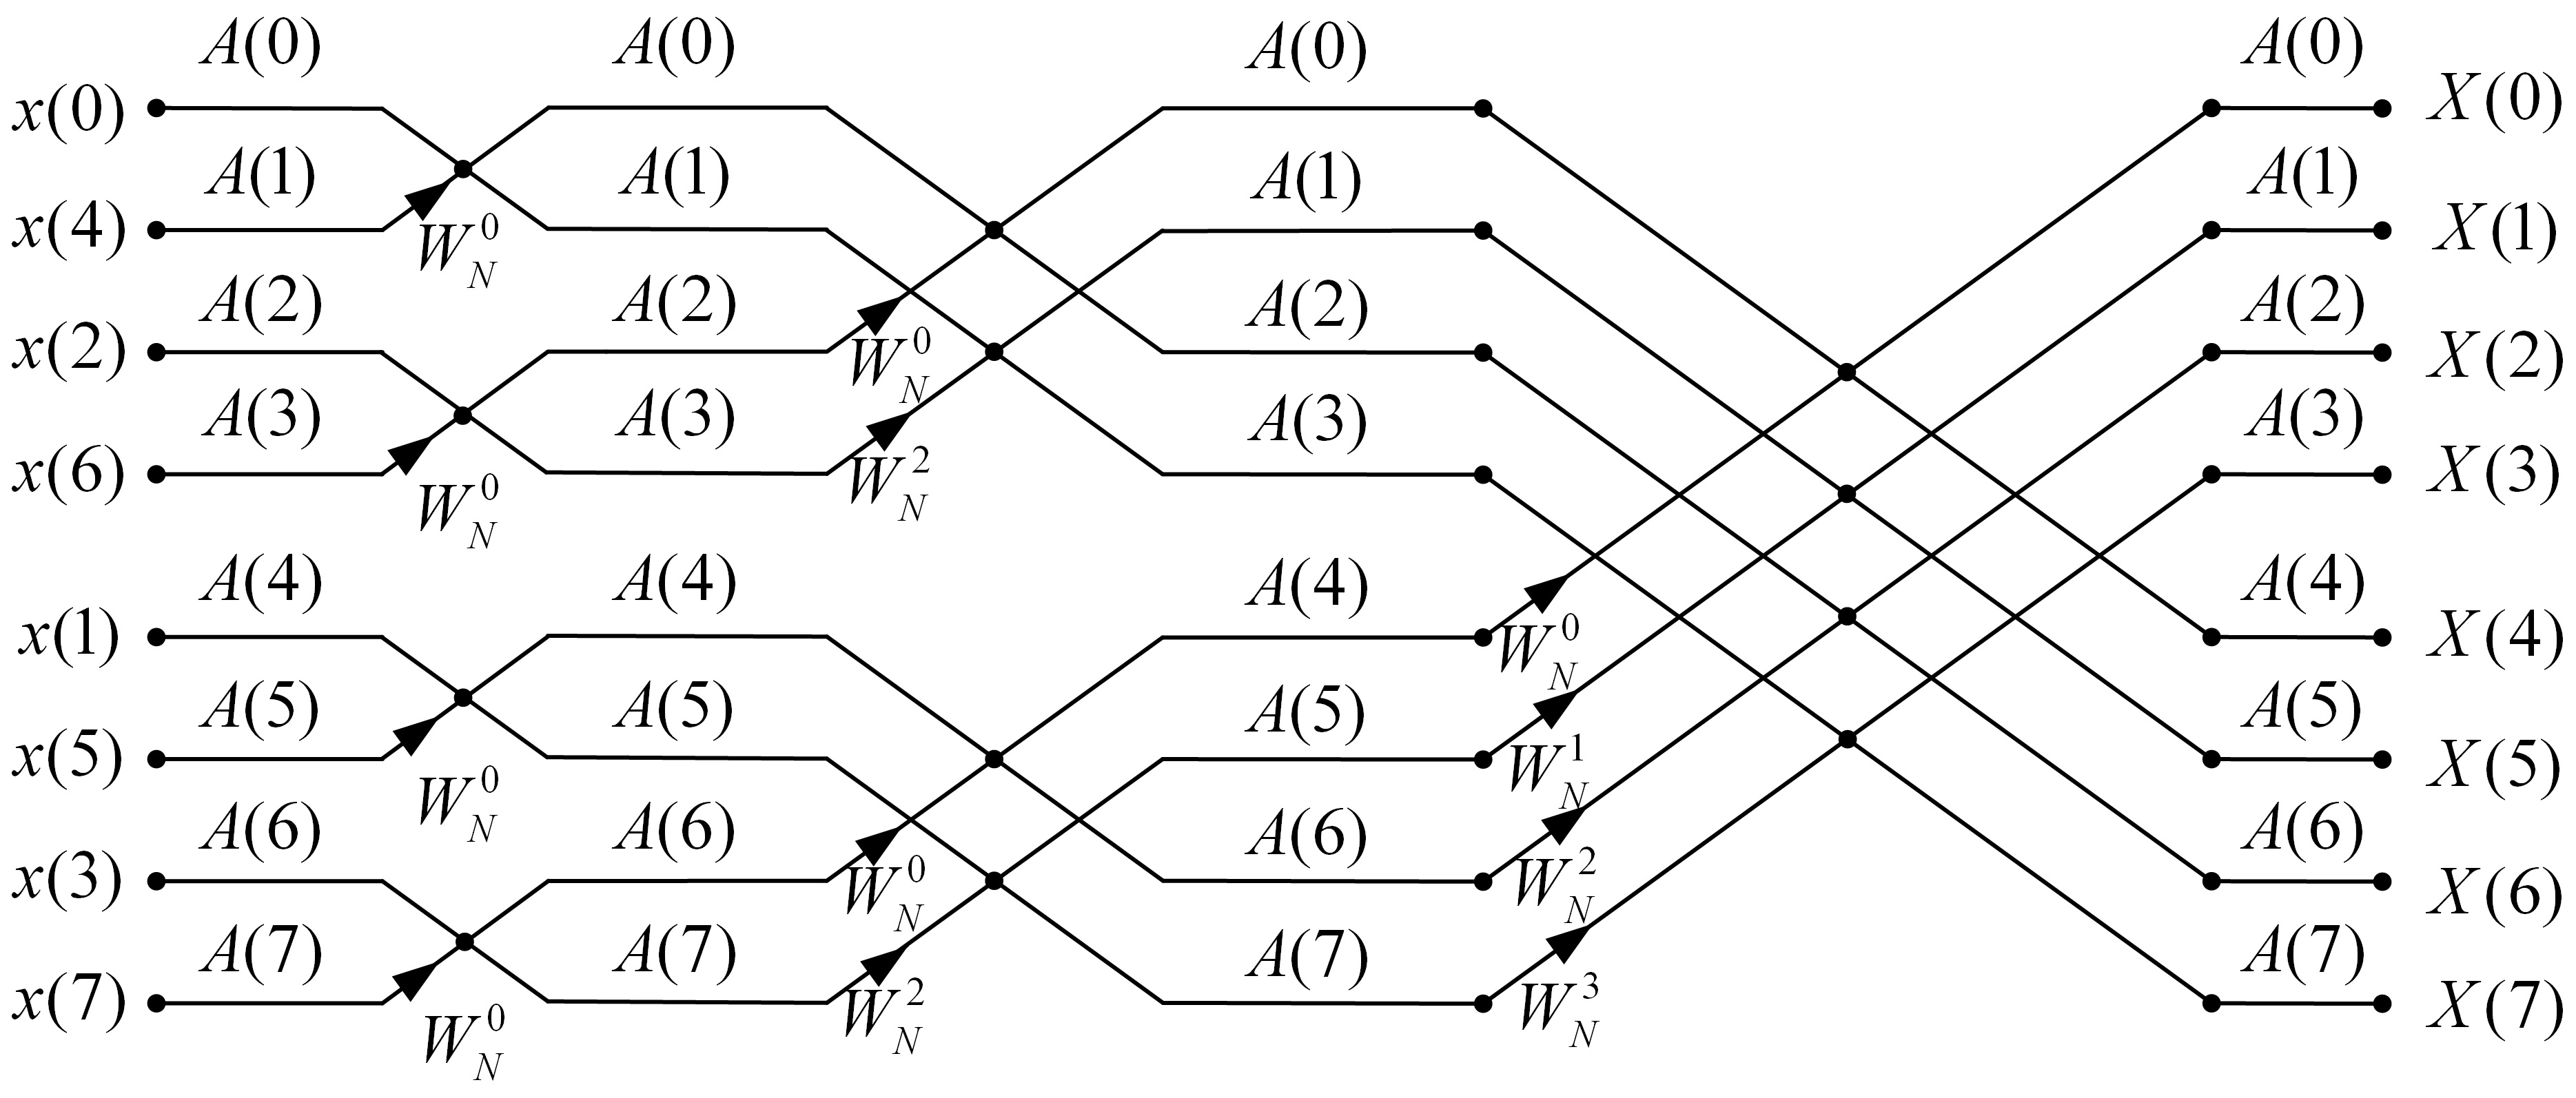
\includegraphics[width=0.99\textwidth]{8dftThird.jpg}
  %\caption{蝶形运算规律}
  %\label{}
\end{figure}
\end{frame}
%%%%%%%%%%%%%%%%%%%%%%%%%%%%%%%%%%%%%%%%%%%%%%%%%%%%%%%%%%%%%%%%%%%%%%%%%%%%%%%%%%%%%%%%%%%%%%%%%%%%%%%%%%%%%%%%%%%%%%%%%
%
%
%
%%%%%%%%%%%%%%%%%%%%%%%%%%%%%%%%%%%%%%%%%%%%%%%%%%%%%%%%%%%%%%%%%%%%%%%%%%%%%%%%%%%%%%%%%%%%%%%%%%%%%%%%%%%%%%%%%%%%%%%%%
%\subsection{蝶形计算}
%%%---------------------------------------------------------------------------------------------------
\begin{frame}[shrink]\frametitle{蝶形运算的计算公式}%[allowframebreaks]
\begin{enumerate}
  \item [1] 在第L级中,每个蝶形两个输入端相距点数为:$B=2^{L-1}$
  %\item [2] 在第L级中,同一个旋转因子,对应相邻间隔为$2^L$点的$2^{M-L}$个蝶形
\end{enumerate}
\begin{equation*}
\left\{ \begin{aligned}
A_{L-1}(J) + W_N^{p}A_{L-1}(J+B) &\longrightarrow A_L(J) \\
A_{L-1}(J) - W_N^{p}A_{L-1}(J+B) &\longrightarrow A_L(J+B)
\end{aligned} \right.
\end{equation*}

\begin{figure}[h]
  \centering
  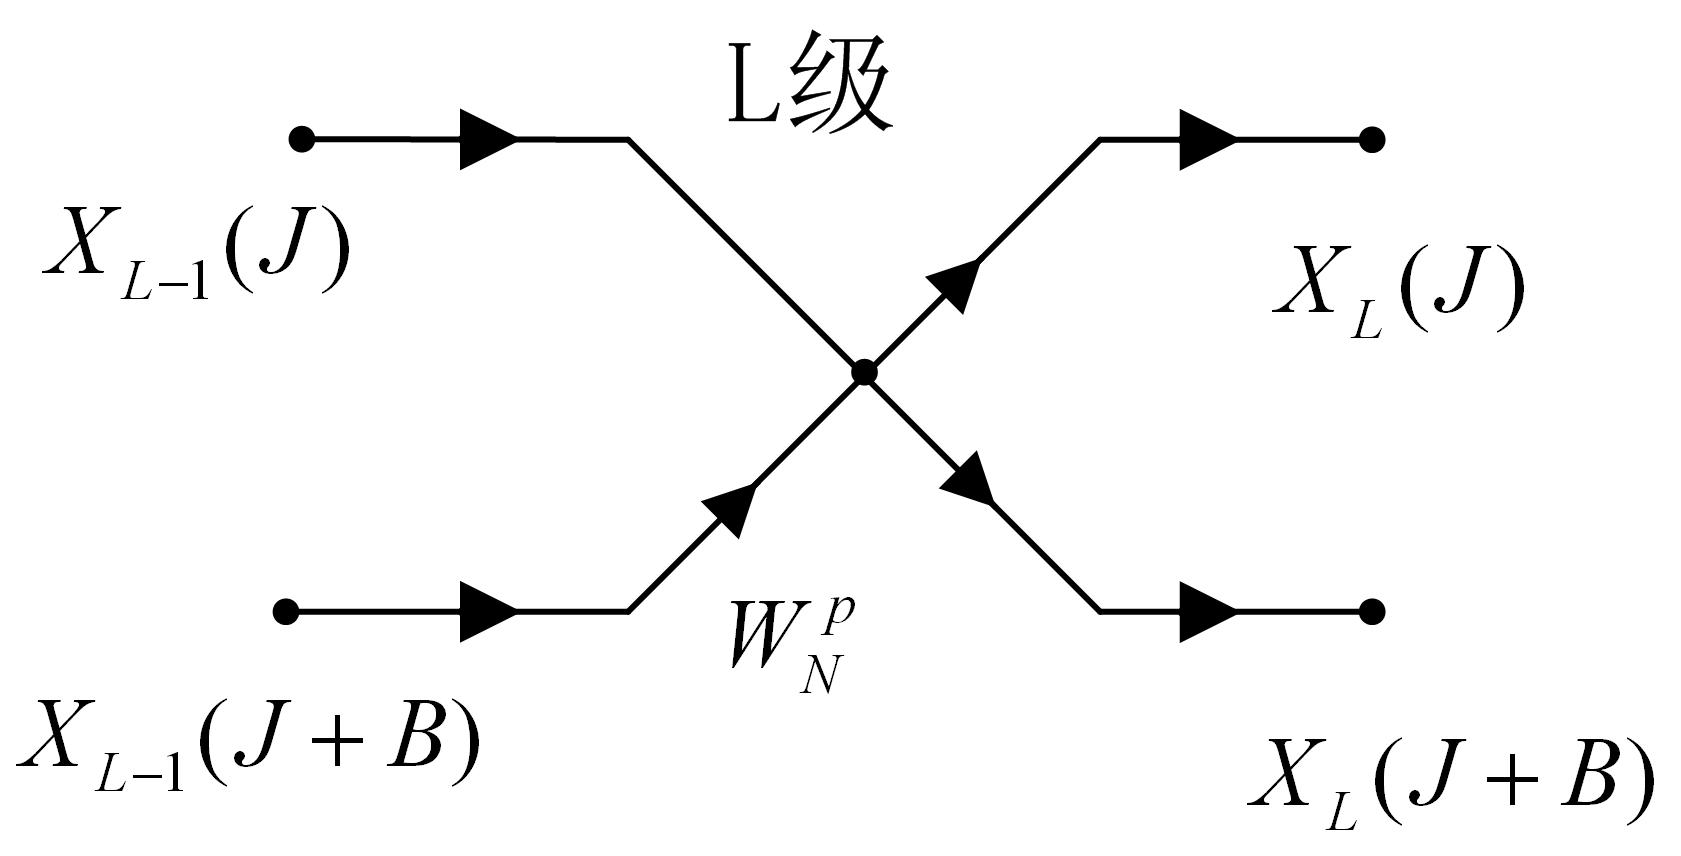
\includegraphics[width=0.5\textwidth]{diexingyunsuanguilv.jpg}
  %\caption{蝶形运算规律}
  %\label{}
\end{figure}
\end{frame}
%%%%%%%%%%%%%%%%%%%%%%%%%%%%%%%%%%%%%%%%%%%%%%%%%%%%%%%%%%%%%%%%%%%%%%%%%%%%%%%%%%%%%%%%%%%%%%%%%%%%%%%%%%%%%%%%%%%%%%%%%
%
%
%
%%%%%%%%%%%%%%%%%%%%%%%%%%%%%%%%%%%%%%%%%%%%%%%%%%%%%%%%%%%%%%%%%%%%%%%%%%%%%%%%%%%%%%%%%%%%%%%%%%%%%%%%%%%%%%%%%%%%%%%%%
\begin{frame}[shrink]\frametitle{说明:容易混淆的情况}%[allowframebreaks]
\begin{enumerate}
  \item [1]两个$2^{L-1}$
  \begin{enumerate}
           \item [(a)] 第L级中,有$B=2^{L-1}$个不同的旋转因子
           \item [(b)] 第L级中,每个蝶形的两个输入端相距的点数$B=2^{L-1}$
  \end{enumerate}
  \item [2] $ 2^{L}\quad$:同一级中具有同一旋转因子的不同蝶形相邻的点数.
\end{enumerate}
\begin{figure}[h]
  \centering
  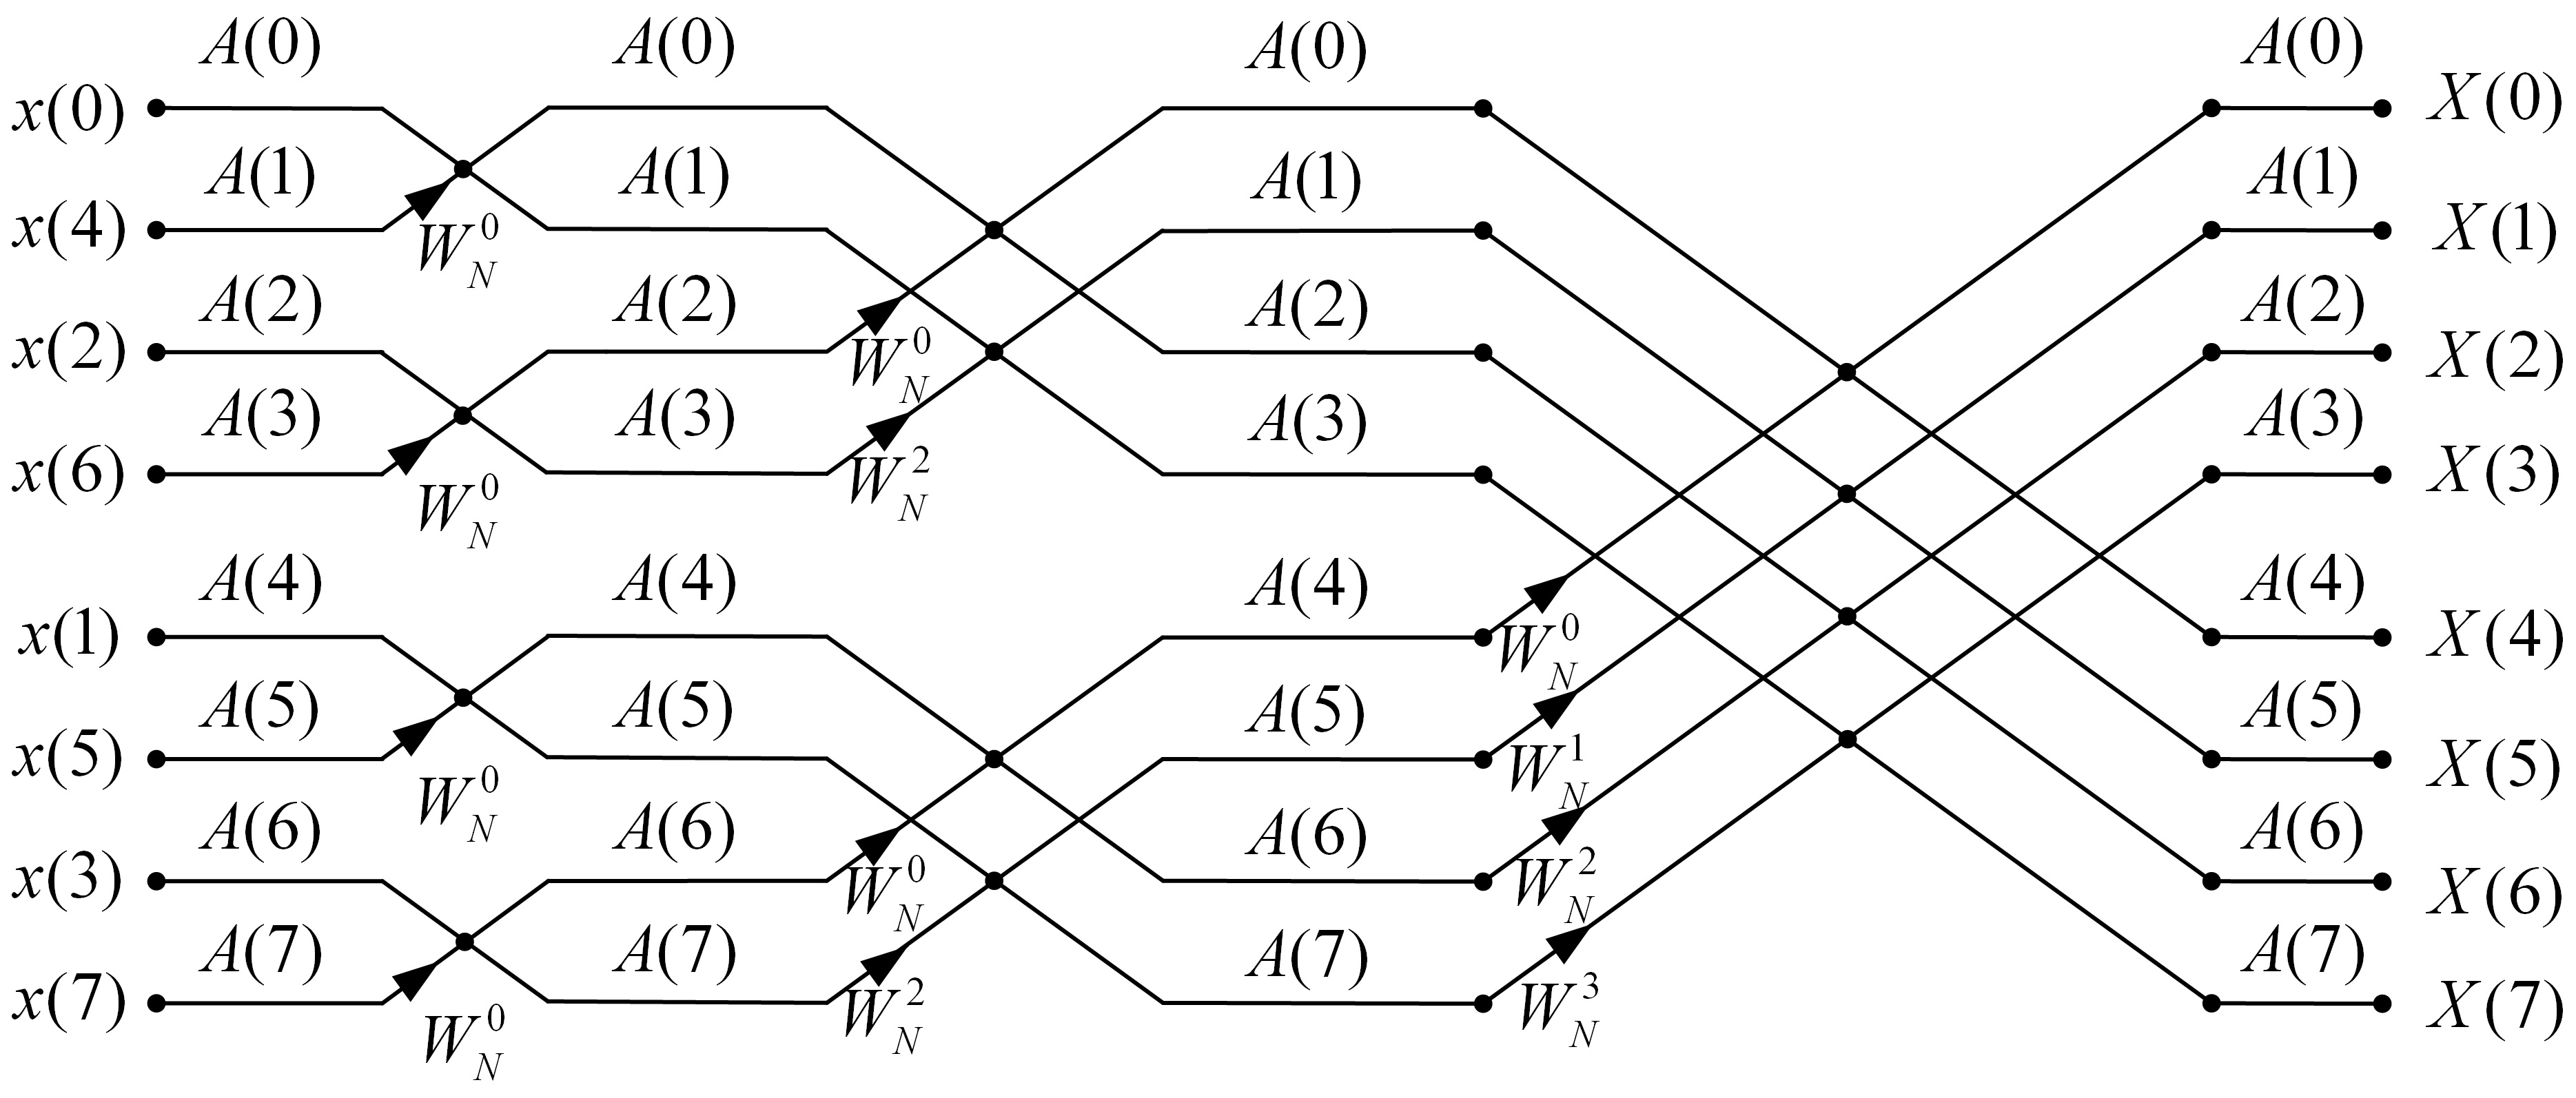
\includegraphics[width=0.9\textwidth]{8dftThird.jpg}
  %\caption{蝶形运算规律}
  %\label{}
\end{figure}
\end{frame}
%%%%%%%%%%%%%%%%%%%%%%%%%%%%%%%%%%%%%%%%%%%%%%%%%%%%%%%%%%%%%%%%%%%%%%%%%%%%%%%%%%%%%%%%%%%%%%%%%%%%%%%%%%%%%%%%%%%%%%%%%%
%%
%%
%%
%%%%%%%%%%%%%%%%%%%%%%%%%%%%%%%%%%%%%%%%%%%%%%%%%%%%%%%%%%%%%%%%%%%%%%%%%%%%%%%%%%%%%%%%%%%%%%%%%%%%%%%%%%%%%%%%%%%%%%%%%%
\subsection{编程思想及程序框图}
%%%%%%%%%%%%%%%%%%%%%%%%%%%%%%%%%%%%%%%%%%%%%%%%%%%%%%%%%%%%%%%%%%%%%%%%%%%%%%%%%%%%%%%%%%%%%%%%%%%%%%%%%%%%%%%%%%%%%%%%%%
%%
%%
%%
%%%%%%%%%%%%%%%%%%%%%%%%%%%%%%%%%%%%%%%%%%%%%%%%%%%%%%%%%%%%%%%%%%%%%%%%%%%%%%%%%%%%%%%%%%%%%%%%%%%%%%%%%%%%%%%%%%%%%%%%%%
\begin{frame}[shrink]\frametitle{总结:第L层旋转因子出现的规律}%[allowframebreaks]
$N=2^M$,共有M级运算,每级有$N/2$个蝶形。
%[蝶形运算规律的总结]
\begin{enumerate}
  \item [1] 第$L$级中,每个蝶形两个输入端相距点数为:$B=2^{L-1}$
  \item [2] 第$L$级中,一共有$2^{L-1}$个不同的旋转因子
  \item [3] 第$L$级中,同一个旋转因子,对应$2^{M-L}$个蝶形,每个蝶形相邻间隔为$2^L$点
\end{enumerate}
%\par 那么将分三个循环进行:
\end{frame}
%%%%%%%%%%%%%%%%%%%%%%%%%%%%%%%%%%%%%%%%%%%%%%%%%%%%%%%%%%%%%%%%%%%%%%%%%%%%%%%%%%%%%%%%%%%%%%%%%%%%%%%%%%%%%%%%%%%%%%%%%%
%%
%%
%%
%%%%%%%%%%%%%%%%%%%%%%%%%%%%%%%%%%%%%%%%%%%%%%%%%%%%%%%%%%%%%%%%%%%%%%%%%%%%%%%%%%%%%%%%%%%%%%%%%%%%%%%%%%%%%%%%%%%%%%%%%%
\begin{frame}[shrink]\frametitle{编程思想}%[allowframebreaks]
那么将分三个循环进行:
\begin{enumerate}
  \item 进行$L=1,2,\cdots,M$级运算。(第一级循环)
  $$L=1,\cdots,M$$
  \item 在第$L$级中,存在$B=2^{L-1}$个旋转因子,按旋转因子不同进行计算。(第二级循环)
  $$B=2^{L-1}$$
  $$J=0,\cdots,B-1$$
  \item 每一个旋转因子对应的$2^{M-L}$个蝶形运算。(第三级循环)
  $$k = J,N-1,2^L$$
  $$(\mbox{k从J开始,每循环一次增加$2^L$,到不超过N-1为止})$$
\end{enumerate}
\end{frame}
%%%%%%%%%%%%%%%%%%%%%%%%%%%%%%%%%%%%%%%%%%%%%%%%%%%%%%%%%%%%%%%%%%%%%%%%%%%%%%%%%%%%%%%%%%%%%%%%%%%%%%%%%%%%%%%%%%%%%%%%%%
%%
%%
%%
%%%%%%%%%%%%%%%%%%%%%%%%%%%%%%%%%%%%%%%%%%%%%%%%%%%%%%%%%%%%%%%%%%%%%%%%%%%%%%%%%%%%%%%%%%%%%%%%%%%%%%%%%%%%%%%%%%%%%%%%%%
\begin{frame}[shrink]\frametitle{举例说明—— 以第二级为例,$L=2$}%[allowframebreaks]
\begin{enumerate}
  \item 计算该层的旋转因子个数,以及每个蝶形相距的点数。
        $$L=2,\quad\quad\therefore B=2^{L-1}=2$$
  \item 计算旋转因子的指数$p$
        $$J=(0,1)\quad\quad\quad p=2^{M-L}\cdot J =2\cdot J=(0,2)$$
  \item 每个旋转因子的蝶形计算,同一旋转因子间隔为$2^L=4$
  $$k=J,7,4$$
  \item 计算公式
  %\begin{enumerate}
    %\item 公式:
    $$
        \left\{ \begin{aligned}
        A_{L-1}(k) + W_N^{p}A_{L-1}(k+B) &\longrightarrow A_L(k)\quad\quad\quad\\
        A_{L-1}(k) - W_N^{p}A_{L-1}(k+B) &\longrightarrow A_L(k+B)
        \end{aligned} \right.
    $$

\end{enumerate}
\end{frame}
%%%%%%%%%%%%%%%%%%%%%%%%%%%%%%%%%%%%%%%%%%%%%%%%%%%%%%%%%%%%%%%%%%%%%%%%%%%%%%%%%%%%%%%%%%%%%%%%%%%%%%%%%%%%%%%%%%%%%%%%%%
%%
%%
%%
%%%%%%%%%%%%%%%%%%%%%%%%%%%%%%%%%%%%%%%%%%%%%%%%%%%%%%%%%%%%%%%%%%%%%%%%%%%%%%%%%%%%%%%%%%%%%%%%%%%%%%%%%%%%%%%%%%%%%%%%%%
\begin{frame}[allowframebreaks]\frametitle{示例 —— 计算过程}%[allowframebreaks]
$$L=2,\quad\quad\therefore B=2^{L-1}=2\quad\quad\quad\quad\quad\quad\quad\quad\quad\quad\quad\quad\quad\quad\quad$$

\begin{enumerate}
  \item [1] $J=0$
      \begin{enumerate}
      \item [(a)] $J=0,p=0,k=0,B=2$
                $$
                    \left\{ \begin{aligned}
                    A(0) + W_N^{0}A(2) &\longrightarrow A(0)\quad\quad\quad\quad\quad\quad\quad\quad \\
                    A(0) - W_N^{0}A(2) &\longrightarrow A(2)
                    \end{aligned} \right.
                $$
      \item [(b)] $J=0,p=0,k=4,B=2$
                $$
                    \left\{ \begin{aligned}
                    A(4) + W_N^{0}A(6) &\longrightarrow A(4)\quad\quad\quad\quad\quad\quad\quad\quad \\
                    A(4) - W_N^{0}A(6) &\longrightarrow A(6)
                    \end{aligned} \right.
                $$
      \end{enumerate}
      \newpage
  \item [2] $J=1$
      \begin{enumerate}
      \item [(a)]$J=1,p=2,k=1,B=2$
                $$
                    \left\{ \begin{aligned}
                    A(1) + W_N^{2}A(3) &\longrightarrow A(1)\quad\quad\quad\quad\quad\quad\quad\quad \\
                    A(1) - W_N^{2}A(3) &\longrightarrow A(3)
                    \end{aligned} \right.
                $$
      \item [(b)]$J=1,p=2,k=5,B=2$
                $$
                    \left\{ \begin{aligned}
                    A(5) + W_N^{2}A(7) &\longrightarrow A(5)\quad\quad\quad\quad\quad\quad\quad\quad \\
                    A(5) - W_N^{2}A(7) &\longrightarrow A(7)
                    \end{aligned} \right.
                $$
      \end{enumerate}
\end{enumerate}
\end{frame}
%%%%%%%%%%%%%%%%%%%%%%%%%%%%%%%%%%%%%%%%%%%%%%%%%%%%%%%%%%%%%%%%%%%%%%%%%%%%%%%%%%%%%%%%%%%%%%%%%%%%%%%%%%%%%%%%%%%%%%%%%%
%%
%%
%%
%%%%%%%%%%%%%%%%%%%%%%%%%%%%%%%%%%%%%%%%%%%%%%%%%%%%%%%%%%%%%%%%%%%%%%%%%%%%%%%%%%%%%%%%%%%%%%%%%%%%%%%%%%%%%%%%%%%%%%%%%%
\subsection{序列的倒序}
\subsubsection{倒序的概念}
%%%%%%%%%%%%%%%%%%%%%%%%%%%%%%%%%%%%%%%%%%%%%%%%%%%%%%%%%%%%%%%%%%%%%%%%%%%%%%%%%%%%%%%%%%%%%%%%%%%%%%%%%%%%%%%%%%%%%%%%%%
%%
%%
%%
%%%%%%%%%%%%%%%%%%%%%%%%%%%%%%%%%%%%%%%%%%%%%%%%%%%%%%%%%%%%%%%%%%%%%%%%%%%%%%%%%%%%%%%%%%%%%%%%%%%%%%%%%%%%%%%%%%%%%%%%%%
\begin{frame}[shrink]\frametitle{倒序的概念}
\begin{enumerate}
  \item DIT-FFT算法流图的输出$X(k)$是自然顺序
  \item 但是,为了适应\textbf{原位计算},其输入序列不是自然顺序,而是经过M次奇偶抽选后的,这样的排序成为序列$x(n)$的倒序。
\end{enumerate}

\begin{figure}[h]
  \centering
  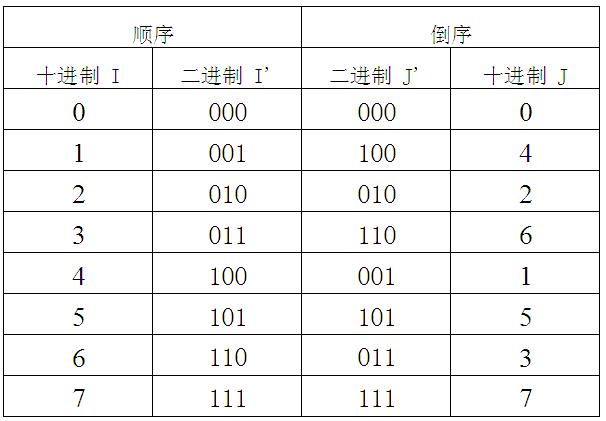
\includegraphics[width=0.6\textwidth]{daoxun.jpg}
  \caption{顺序和倒序二进制对照表}
  %\label{}
\end{figure}
\end{frame}
%%%%%%%%%%%%%%%%%%%%%%%%%%%%%%%%%%%%%%%%%%%%%%%%%%%%%%%%%%%%%%%%%%%%%%%%%%%%%%%%%%%%%%%%%%%%%%%%%%%%%%%%%%%%%%%%%%%%%%%%%%
%%
%%
%%
%%%%%%%%%%%%%%%%%%%%%%%%%%%%%%%%%%%%%%%%%%%%%%%%%%%%%%%%%%%%%%%%%%%%%%%%%%%%%%%%%%%%%%%%%%%%%%%%%%%%%%%%%%%%%%%%%%%%%%%%%%
\begin{frame}[shrink]\frametitle{顺序数与倒序数的不同特点}%[allowframebreaks]
关键:若已知当前倒序数$J$,如何得到下一个倒序数。
顺序数与倒序数的不同特点
\begin{itemize}
  \item 顺序数二进制在最低位加1,向左进位。
  \item 倒序数二进制在最高位加1,向右进位。
\end{itemize}
\begin{figure}[h]
  \centering
  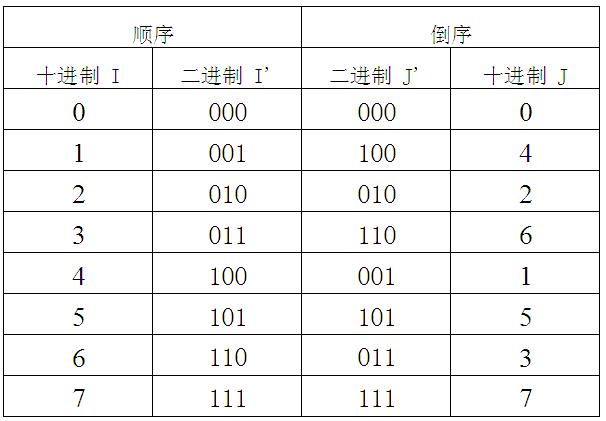
\includegraphics[width=0.6\textwidth]{daoxun.jpg}
  %\caption{顺序和倒序二进制对照表}
  %\label{}
\end{figure}
\end{frame}
%%%%%%%%%%%%%%%%%%%%%%%%%%%%%%%%%%%%%%%%%%%%%%%%%%%%%%%%%%%%%%%%%%%%%%%%%%%%%%%%%%%%%%%%%%%%%%%%%%%%%%%%%%%%%%%%%%%%%%%%%%
%%
%%
%%
%%%%%%%%%%%%%%%%%%%%%%%%%%%%%%%%%%%%%%%%%%%%%%%%%%%%%%%%%%%%%%%%%%%%%%%%%%%%%%%%%%%%%%%%%%%%%%%%%%%%%%%%%%%%%%%%%%%%%%%%%%
\begin{frame}[shrink]\frametitle{8点DIT-FFT运算流图}%[allowframebreaks]
编程:已知当前十进制$J$,在$J'$中考察
\begin{enumerate}
  \item [(1)]若$J'$最高位为0,则$J+\frac{N}{2}\longrightarrow J$
            \newline

  \item [(2)]若$J'$最高位为1,则$J-\frac{N}{2}\longrightarrow J$,向右进一位。
  \newline
    \begin{figure}[h]
    \centering
    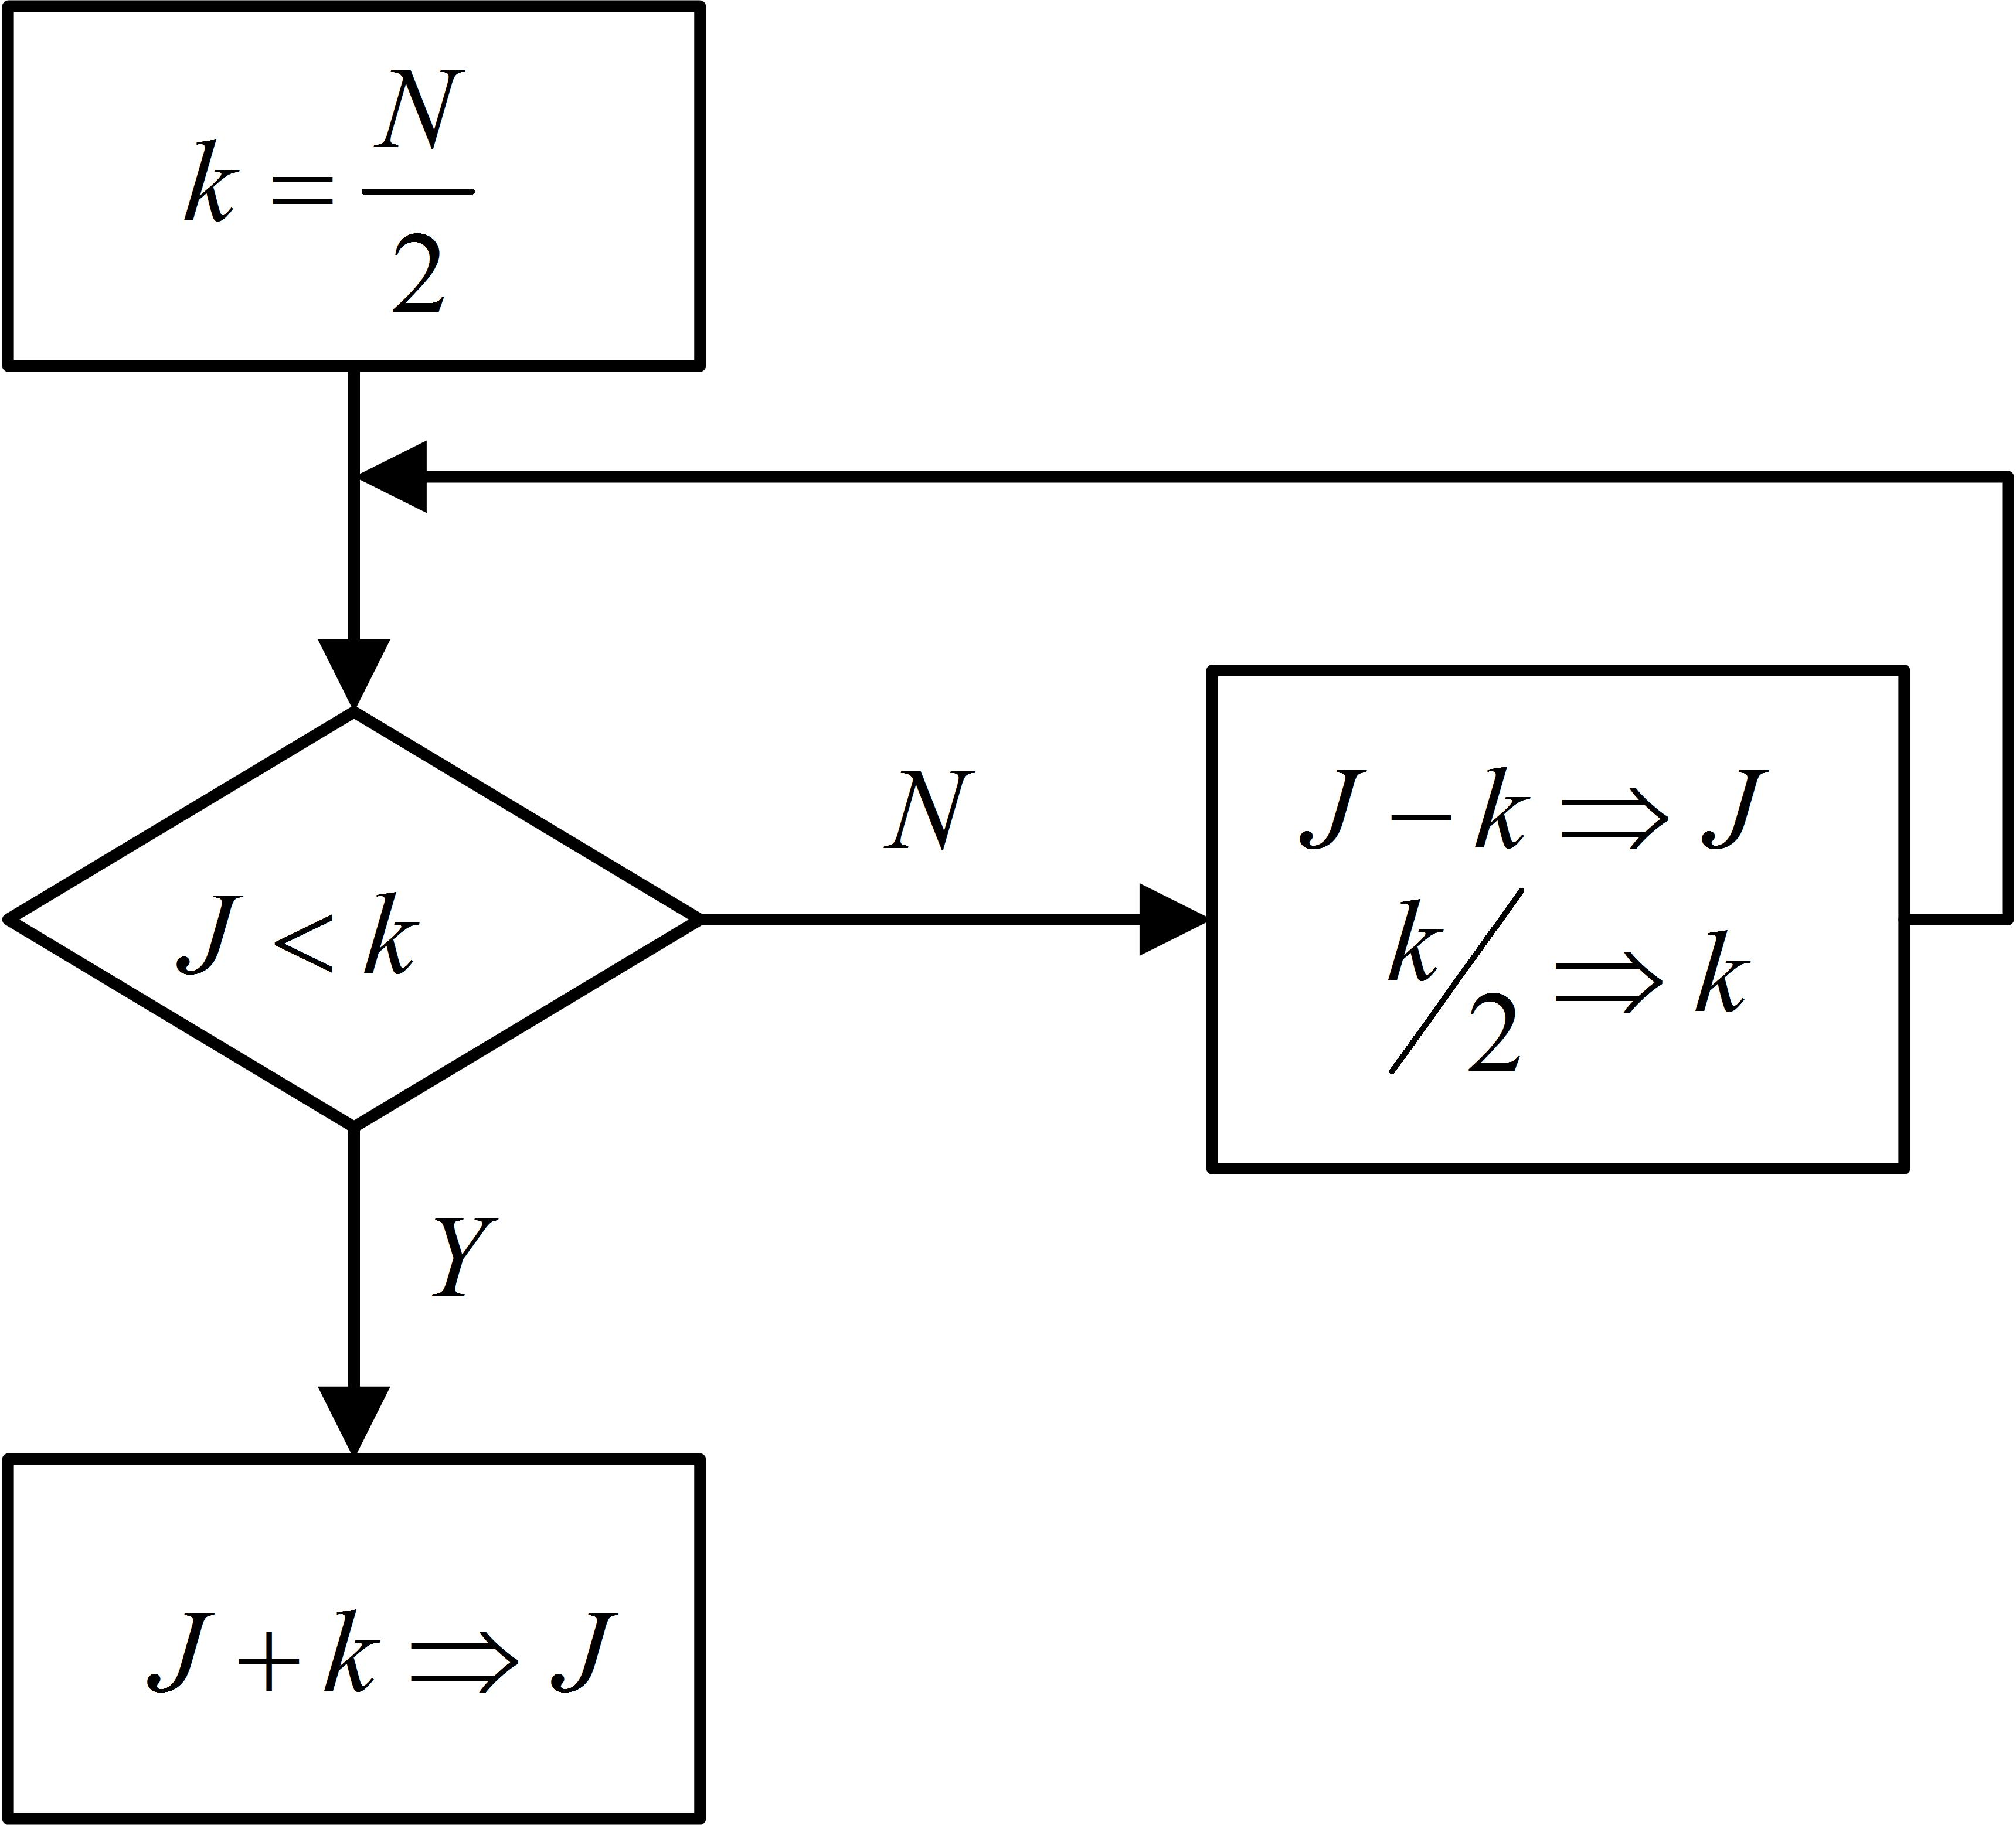
\includegraphics[width=0.5\textwidth]{daoxubianchen.jpg}
    %\caption{倒序程序框图简图}
    %\label{}
    \end{figure}
\end{enumerate}
\end{frame}
%%%%%%%%%%%%%%%%%%%%%%%%%%%%%%%%%%%%%%%%%%%%%%%%%%%%%%%%%%%%%%%%%%%%%%%%%%%%%%%%%%%%%%%%%%%%%%%%%%%%%%%%%%%%%%%%%%%%%%%%%%
%%
%%
%%
%%%%%%%%%%%%%%%%%%%%%%%%%%%%%%%%%%%%%%%%%%%%%%%%%%%%%%%%%%%%%%%%%%%%%%%%%%%%%%%%%%%%%%%%%%%%%%%%%%%%%%%%%%%%%%%%%%%%%%%%%%
\subsubsection{倒序的编程思想及程序框图}
%%%%%%%%%%%%%%%%%%%%%%%%%%%%%%%%%%%%%%%%%%%%%%%%%%%%%%%%%%%%%%%%%%%%%%%%%%%%%%%%%%%%%%%%%%%%%%%%%%%%%%%%%%%%%%%%%%%%%%%%%
%
%
%
%%%%%%%%%%%%%%%%%%%%%%%%%%%%%%%%%%%%%%%%%%%%%%%%%%%%%%%%%%%%%%%%%%%%%%%%%%%%%%%%%%%%%%%%%%%%%%%%%%%%%%%%%%%%%%%%%%%%%%%%%%
\begin{frame}[shrink]\frametitle{对$x(n)$按倒序重新排列}%[allowframebreaks]
形成倒序后,我们已经知道倒序序列的组成。下一个问题是将原数组A中存放的输入
序列重新按倒序排列。
\begin{figure}[h]
\centering
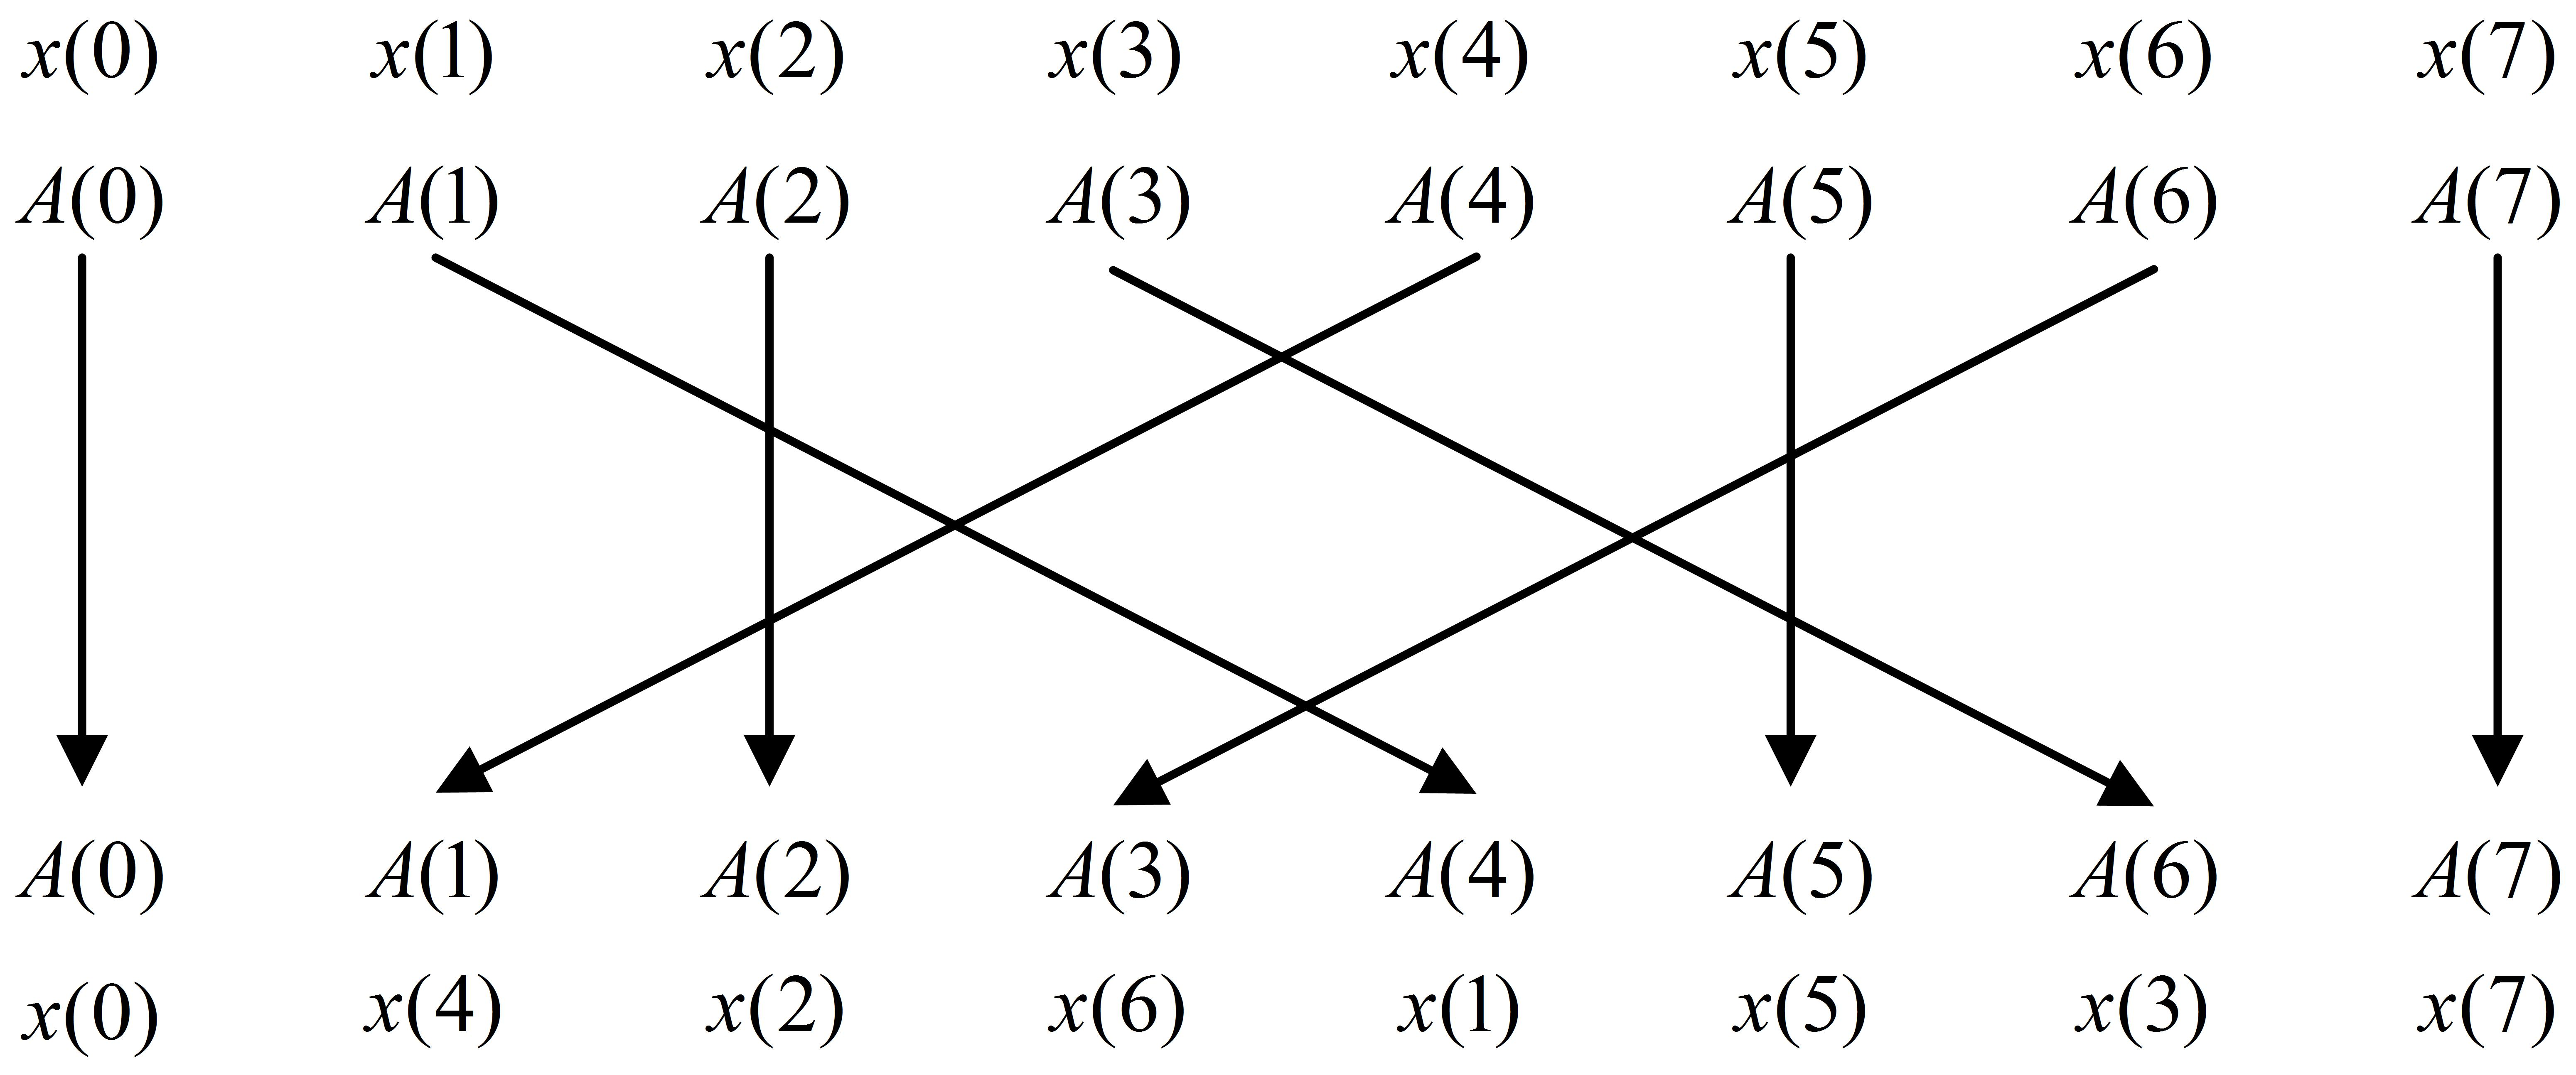
\includegraphics[width=0.8\textwidth]{daoxuguilv.jpg}
%\caption{倒序规律}
%\label{}
\end{figure}
\begin{enumerate}
  \item $x(0),x(N-1)$不动。
  \item 当$I=J$时,不动。
  \item 当$I\neq J$时,$A(I)$和$A(J)$交换数据。
\end{enumerate}

\end{frame}
%%%%%%%%%%%%%%%%%%%%%%%%%%%%%%%%%%%%%%%%%%%%%%%%%%%%%%%%%%%%%%%%%%%%%%%%%%%%%%%%%%%%%%%%%%%%%%%%%%%%%%%%%%%%%%%%%%%%%%%%%
%
%
%
%%%%%%%%%%%%%%%%%%%%%%%%%%%%%%%%%%%%%%%%%%%%%%%%%%%%%%%%%%%%%%%%%%%%%%%%%%%%%%%%%%%%%%%%%%%%%%%%%%%%%%%%%%%%%%%%%%%%%%%%%%
\section{频域抽取法(DIF-FFT)}
\subsection{频域抽取法(DIF-FFT)}
%%%%%%%%%%%%%%%%%%%%%%%%%%%%%%%%%%%%%%%%%%%%%%%%%%%%%%%%%%%%%%%%%%%%%%%%%%%%%%%%%%%%%%%%%%%%%%%%%%%%%%%%%%%%%%%%%%%%%%%%%%
%%
%%
%%
%%%%%%%%%%%%%%%%%%%%%%%%%%%%%%%%%%%%%%%%%%%%%%%%%%%%%%%%%%%%%%%%%%%%%%%%%%%%%%%%%%%%%%%%%%%%%%%%%%%%%%%%%%%%%%%%%%%%%%%%%%
\begin{frame}[shrink]\frametitle{频域域抽取法基2FFT将长序列分解为短序列所遵循的原则}%[allowframebreaks]
\begin{enumerate}
  \item 对时间前后分(n)
  \item 对频率分奇偶(k)
\end{enumerate}
\end{frame}
%%%%%%%%%%%%%%%%%%%%%%%%%%%%%%%%%%%%%%%%%%%%%%%%%%%%%%%%%%%%%%%%%%%%%%%%%%%%%%%%%%%%%%%%%%%%%%%%%%%%%%%%%%%%%%%%%%%%%%%%%%
%%
%%
%%
%%%%%%%%%%%%%%%%%%%%%%%%%%%%%%%%%%%%%%%%%%%%%%%%%%%%%%%%%%%%%%%%%%%%%%%%%%%%%%%%%%%%%%%%%%%%%%%%%%%%%%%%%%%%%%%%%%%%%%%%%%
\begin{frame}\frametitle{}%[allowframebreaks]

\par 假设序列$x(n)$长度为N,且满足$N=2^{M}$,M为自然数。(不是的补0)
\par 按n的前后把$x(n)$分解为两个$N/2$长的子序列
    \begin{equation*} \label{eq:4}
    \begin{split}
    X(k)&= DFT[x(n)] \\
        &= \sum_{n=0}^{N-1}x(n)W_{N}^{kn},\quad\quad\quad (0\leq k\leq N-1)\\
        &= \sum_{n=0}^{\frac{N}{2}-1}x(n)W_{N}^{kn} +\sum_{n=\frac{N}{2}}^{N-1}x(n)W_{N}^{kn}\\
    \end{split}
    \end{equation*}
\end{frame}
%%%%%%%%%%%%%%%%%%%%%%%%%%%%%%%%%%%%%%%%%%%%%%%%%%%%%%%%%%%%%%%%%%%%%%%%%%%%%%%%%%%%%%%%%%%%%%%%%%%%%%%%%%%%%%%%%%%%%%%%%%
%%
%%
%%
%%%%%%%%%%%%%%%%%%%%%%%%%%%%%%%%%%%%%%%%%%%%%%%%%%%%%%%%%%%%%%%%%%%%%%%%%%%%%%%%%%%%%%%%%%%%%%%%%%%%%%%%%%%%%%%%%%%%%%%%%%
\begin{frame}\frametitle{}%[allowframebreaks]

\quad\quad\quad\quad 令$n=n_1+\frac{N}{2}$,则有:
    \begin{equation*} \label{eq:4}
    \begin{split}
    \sum_{n=\frac{N}{2}}^{N-1}x(n)W_{N}^{kn}
        &= \sum_{n_1=0}^{\frac{N}{2}-1}x(n_1+\frac{N}{2})W_{N}^{k(n_1+\frac{N}{2})} \\
        &\quad  \quad\quad\quad \mbox{(将$n_1$替换为$n$)}\\
        &= \sum_{n=0}^{\frac{N}{2}-1}x(n+\frac{N}{2})W_{N}^{\frac{N}{2}k}W_{N}^{kn} \\
    \end{split}
    \end{equation*}
$$X(k)= \sum_{n=0}^{\frac{N}{2}-1}x(n)W_{N}^{kn} +
       \sum_{n=0}^{\frac{N}{2}-1}x(n+\frac{N}{2})W_{N}^{\frac{N}{2}k}W_{N}^{kn}$$

$$\mbox{注意:\quad\quad}  W_{N}^{\frac{N}{2}k} = (W_{N}^{\frac{N}{2}})^k = (-1)^k$$
\end{frame}
%%%%%%%%%%%%%%%%%%%%%%%%%%%%%%%%%%%%%%%%%%%%%%%%%%%%%%%%%%%%%%%%%%%%%%%%%%%%%%%%%%%%%%%%%%%%%%%%%%%%%%%%%%%%%%%%%%%%%%%%%%
%%
%%
%%
%%%%%%%%%%%%%%%%%%%%%%%%%%%%%%%%%%%%%%%%%%%%%%%%%%%%%%%%%%%%%%%%%%%%%%%%%%%%%%%%%%%%%%%%%%%%%%%%%%%%%%%%%%%%%%%%%%%%%%%%%%
\begin{frame}\frametitle{}%[allowframebreaks]
\begin{equation*}
\begin{split}
X(k)&= \sum_{n=0}^{\frac{N}{2}-1}x(n)W_{N}^{kn} +
       \sum_{n=0}^{\frac{N}{2}-1}x(n+\frac{N}{2})W_{N}^{\frac{N}{2}k}W_{N}^{kn}\\
    &= \sum_{n=0}^{\frac{N}{2}-1}\left[x(n)+W_{N}^{\frac{N}{2}k}x(n+\frac{N}{2})\right]W_{N}^{kn}\\
    &= \sum_{n=0}^{\frac{N}{2}-1}\left[x(n)+(-1)^kx(n+\frac{N}{2})\right]W_{N}^{kn}
    \quad\quad(0\leq k\leq N-1)\\
\end{split}
\end{equation*}
\end{frame}
%%%%%%%%%%%%%%%%%%%%%%%%%%%%%%%%%%%%%%%%%%%%%%%%%%%%%%%%%%%%%%%%%%%%%%%%%%%%%%%%%%%%%%%%%%%%%%%%%%%%%%%%%%%%%%%%%%%%%%%%%%
%%
%%
%%
%%%%%%%%%%%%%%%%%%%%%%%%%%%%%%%%%%%%%%%%%%%%%%%%%%%%%%%%%%%%%%%%%%%%%%%%%%%%%%%%%%%%%%%%%%%%%%%%%%%%%%%%%%%%%%%%%%%%%%%%%%
\begin{frame}\frametitle{}%[allowframebreaks]
对频率$\quad k\quad$奇偶分
\begin{equation*} \label{eq:2}
\left\{ \begin{aligned}
k &= 2m \\
k &= 2m+1
\end{aligned} \right.
\end{equation*}
则:
$$X(2m)=\sum_{n=0}^{\frac{N}{2}-1}\left[x(n)+x(n+\frac{N}{2})\right]W_{N}^{2mn}$$
$$X(2m+1)=\sum_{n=0}^{\frac{N}{2}-1}\left[x(n)-x(n+\frac{N}{2})\right]W_{N}^{(2m+1)n}$$
而:$$W_N^{(2m+1)n}=W_{\frac{N}{2}}^{mn}W_N^n$$
\end{frame}
%%%%%%%%%%%%%%%%%%%%%%%%%%%%%%%%%%%%%%%%%%%%%%%%%%%%%%%%%%%%%%%%%%%%%%%%%%%%%%%%%%%%%%%%%%%%%%%%%%%%%%%%%%%%%%%%%%%%%%%%%%
%%
%%
%%
%%%%%%%%%%%%%%%%%%%%%%%%%%%%%%%%%%%%%%%%%%%%%%%%%%%%%%%%%%%%%%%%%%%%%%%%%%%%%%%%%%%%%%%%%%%%%%%%%%%%%%%%%%%%%%%%%%%%%%%%%%
\begin{frame}\frametitle{}%[allowframebreaks]


最后得到:
\begin{equation*} \label{eq:2}
\left \{
\begin{aligned}
    X(2m)\quad &= \sum_{n=0}^{\frac{N}{2}-1}\left[x(n)+x(n+\frac{N}{2})\right]W_{\frac{N}{2}}^{mn} \quad\quad(0\leq m\leq\frac{N}{2}-1)\\
    X(2m+1)    &= \sum_{n=0}^{\frac{N}{2}-1}\left[(x(n)-x(n+\frac{N}{2}))W_N^n \right]W_{\frac{N}{2}}^{mn}\\
\end{aligned}
\right.
\end{equation*}
令,
$$
\left \{
\begin{aligned}
    x_1(n)&= x(n)+x(n+\frac{N}{2})\quad\quad(0\leq n\leq\frac{N}{2}-1)\quad\quad\quad\quad\quad\quad\quad\quad\\
    x_2(n)&= \left[x(n)-x(n+\frac{N}{2})\right]W_N^n\\
\end{aligned}
\right.
$$
\end{frame}
%%%%%%%%%%%%%%%%%%%%%%%%%%%%%%%%%%%%%%%%%%%%%%%%%%%%%%%%%%%%%%%%%%%%%%%%%%%%%%%%%%%%%%%%%%%%%%%%%%%%%%%%%%%%%%%%%%%%%%%%%%
%%
%%
%%
%%%%%%%%%%%%%%%%%%%%%%%%%%%%%%%%%%%%%%%%%%%%%%%%%%%%%%%%%%%%%%%%%%%%%%%%%%%%%%%%%%%%%%%%%%%%%%%%%%%%%%%%%%%%%%%%%%%%%%%%%%
\begin{frame}\frametitle{}%[allowframebreaks]
$$\mbox{令}\quad\quad DFT[x_1(n)]=X_1(k)\quad\quad\quad\quad DFT\left[x_2(n)\right]=X_2(k)$$
则有:
$$
\left \{
\begin{aligned}
    X_1(k)&= X(2k)\quad\quad(0\leq k\leq\frac{N}{2}-1)
    \quad\quad\quad\quad\quad\quad\quad\quad\quad\quad\\
    X_2(k)&= X(2k+1)\\
\end{aligned}
\right.
$$
DIF-FFT蝶形运算符号:
\begin{figure}[h]
  \centering
  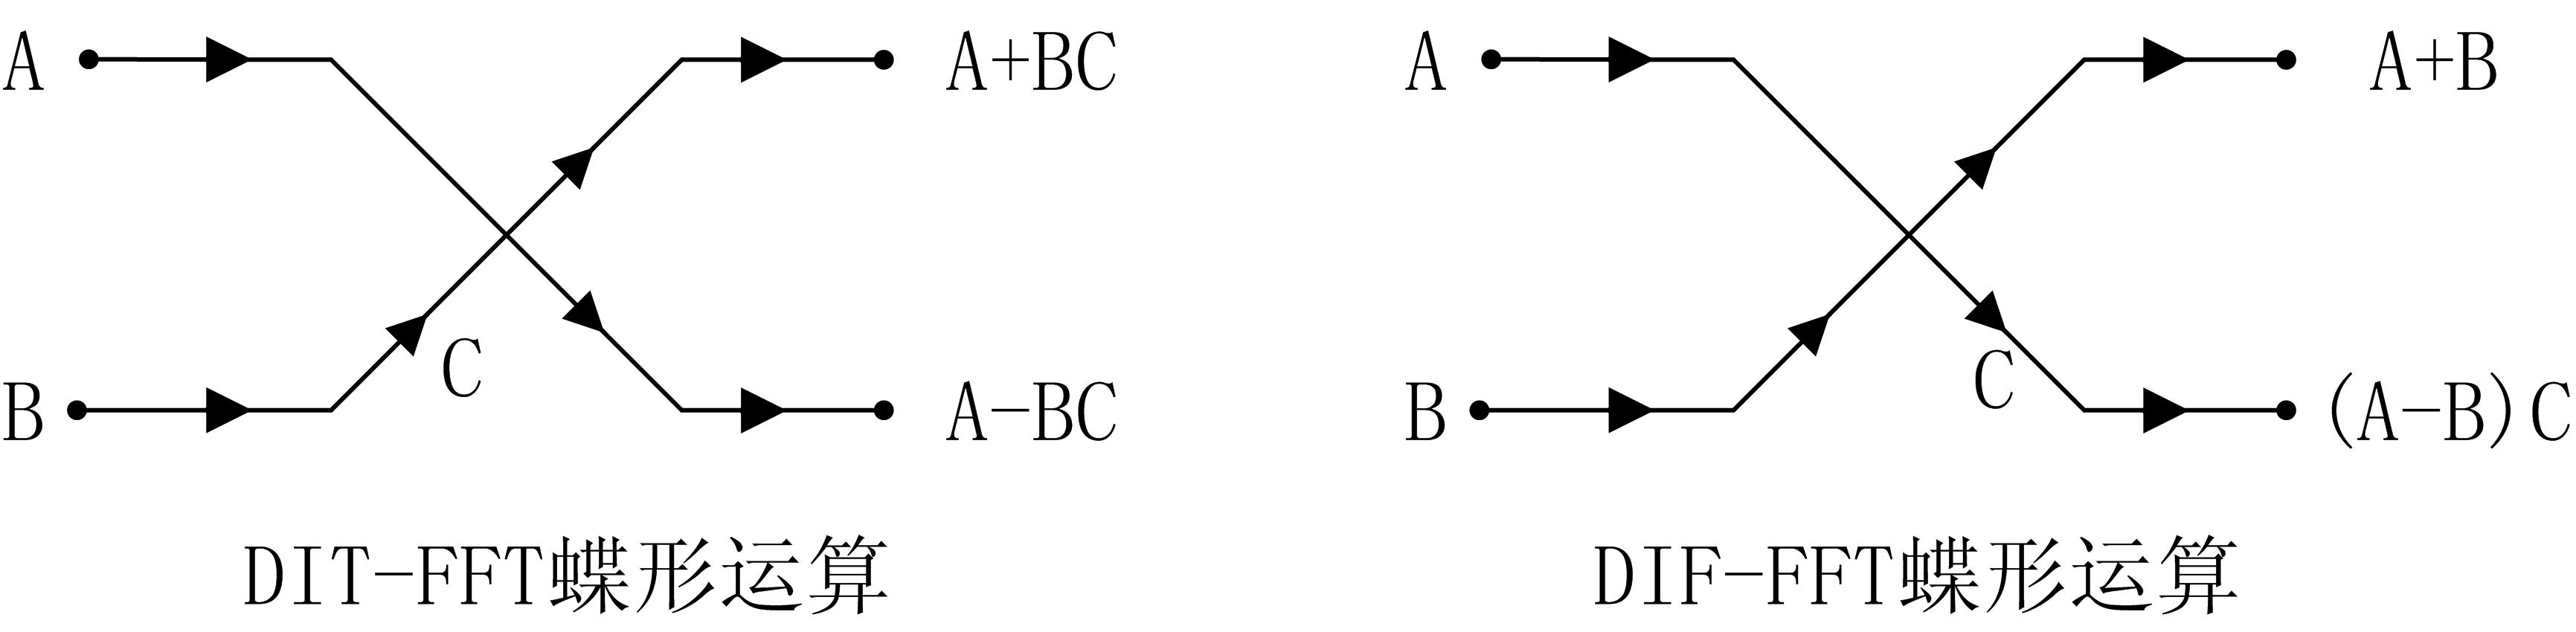
\includegraphics[width=0.8\textwidth]{Diffftdiexing.jpg}
  %\caption{蝶形运算符号}
\end{figure}
\end{frame}


\begin{frame}\frametitle{8点DIF-DFT一次时域分解运算流图}%[allowframebreaks]
\begin{figure}[h]
  \centering
  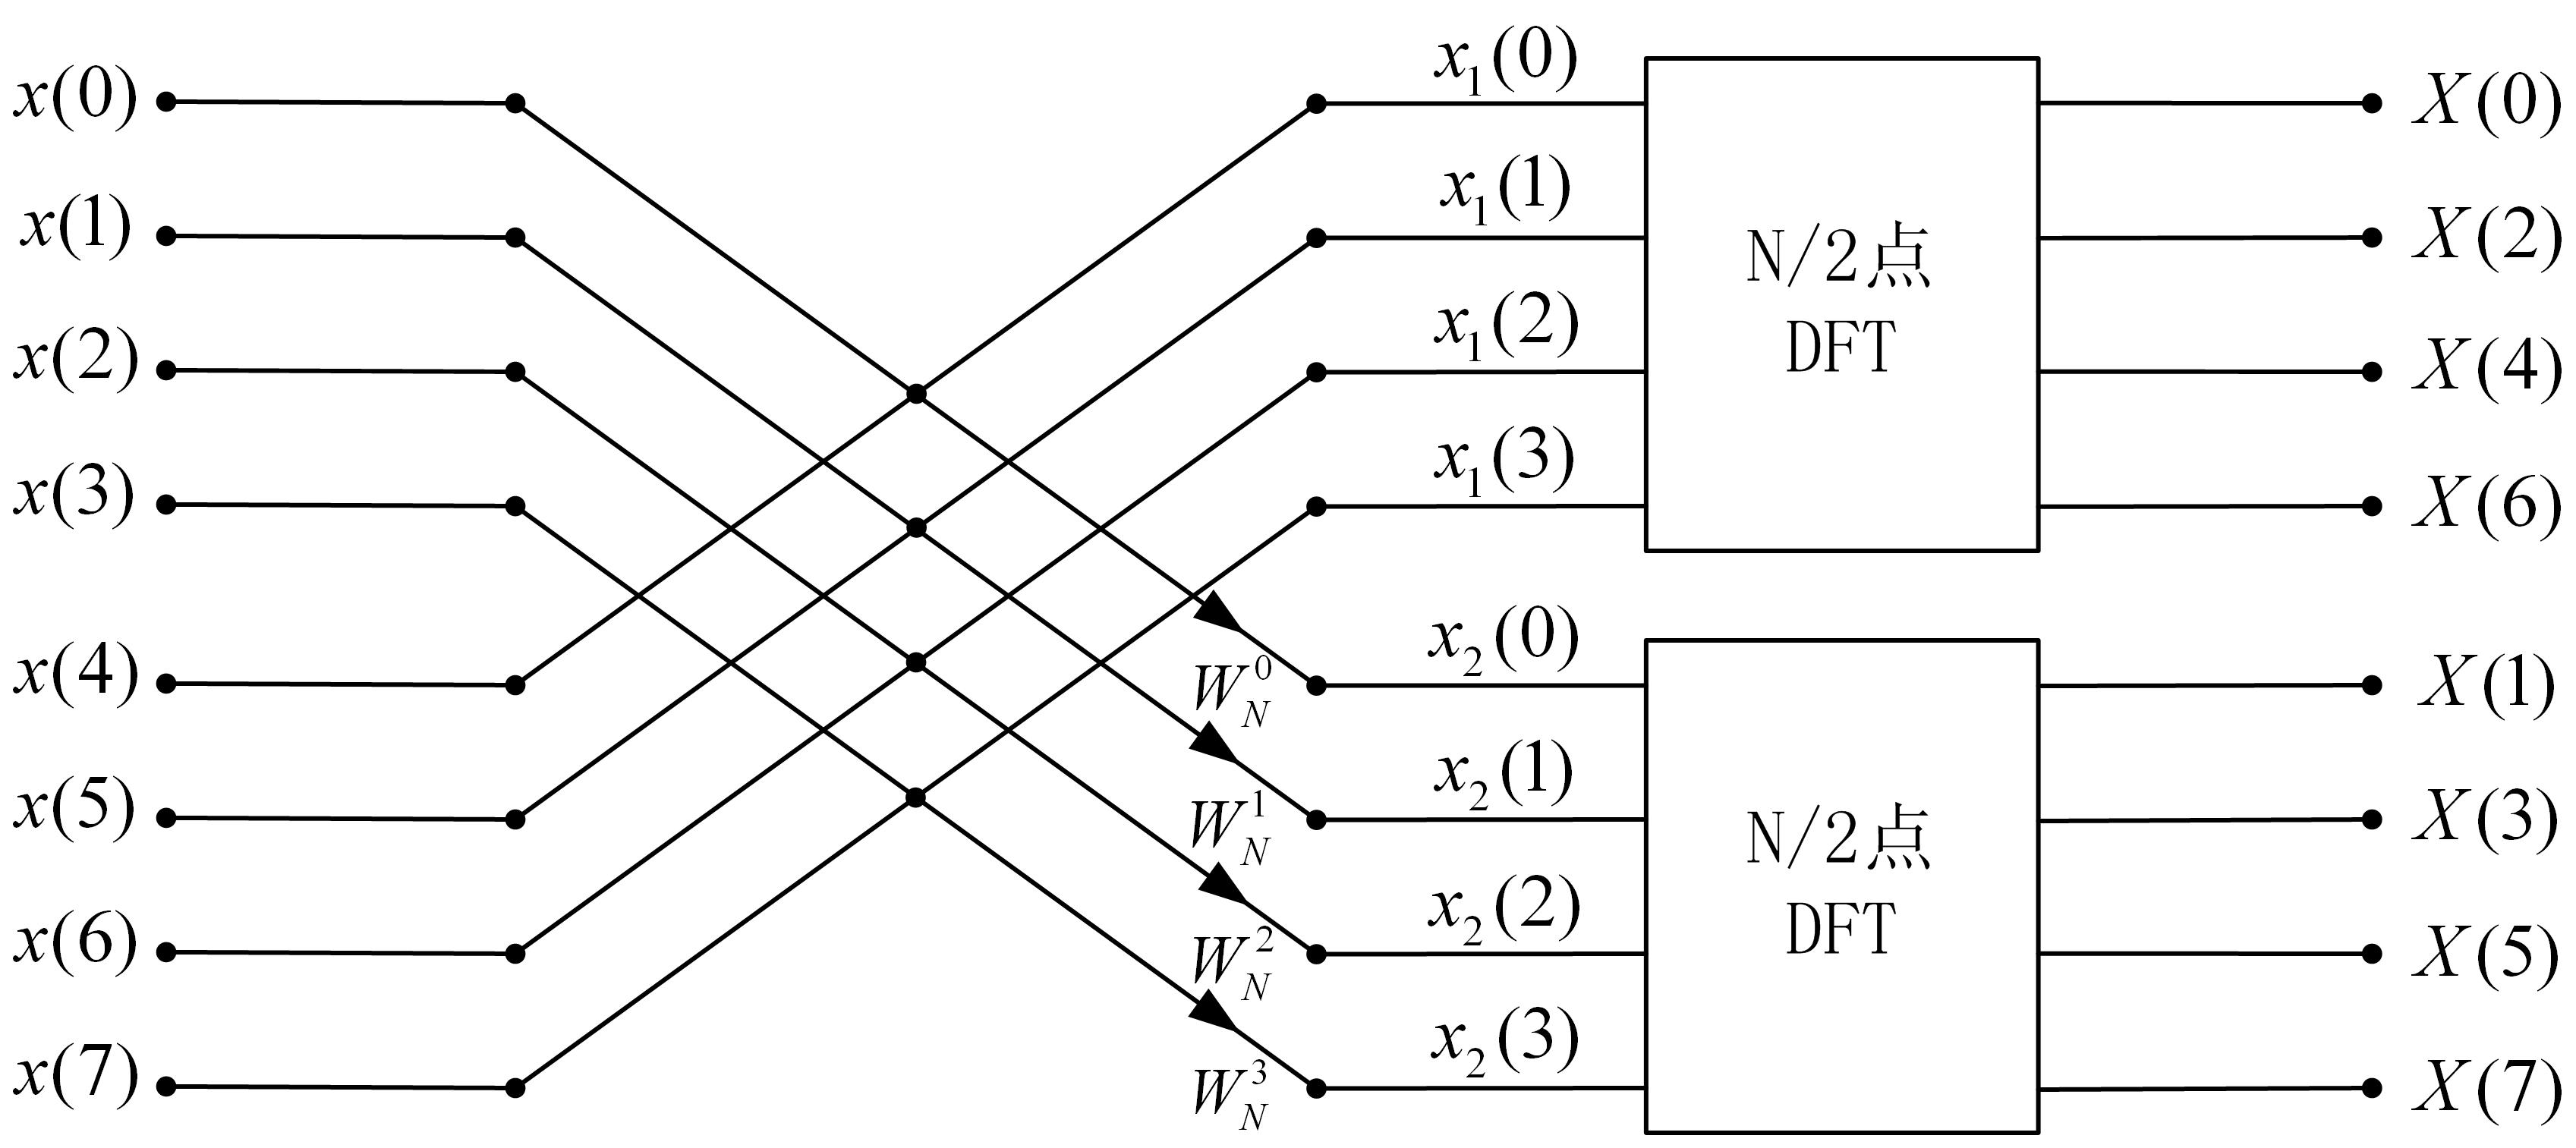
\includegraphics[width=0.99\textwidth]{dif8dftFirst.jpg}
  %\caption{8点DIF-DFT一次时域分解运算流图}
  %\label{}
\end{figure}
\end{frame}

\begin{frame}\frametitle{8点DIF-DFT二次时域分解运算流图}%[allowframebreaks]
\begin{figure}[h]
  \centering
  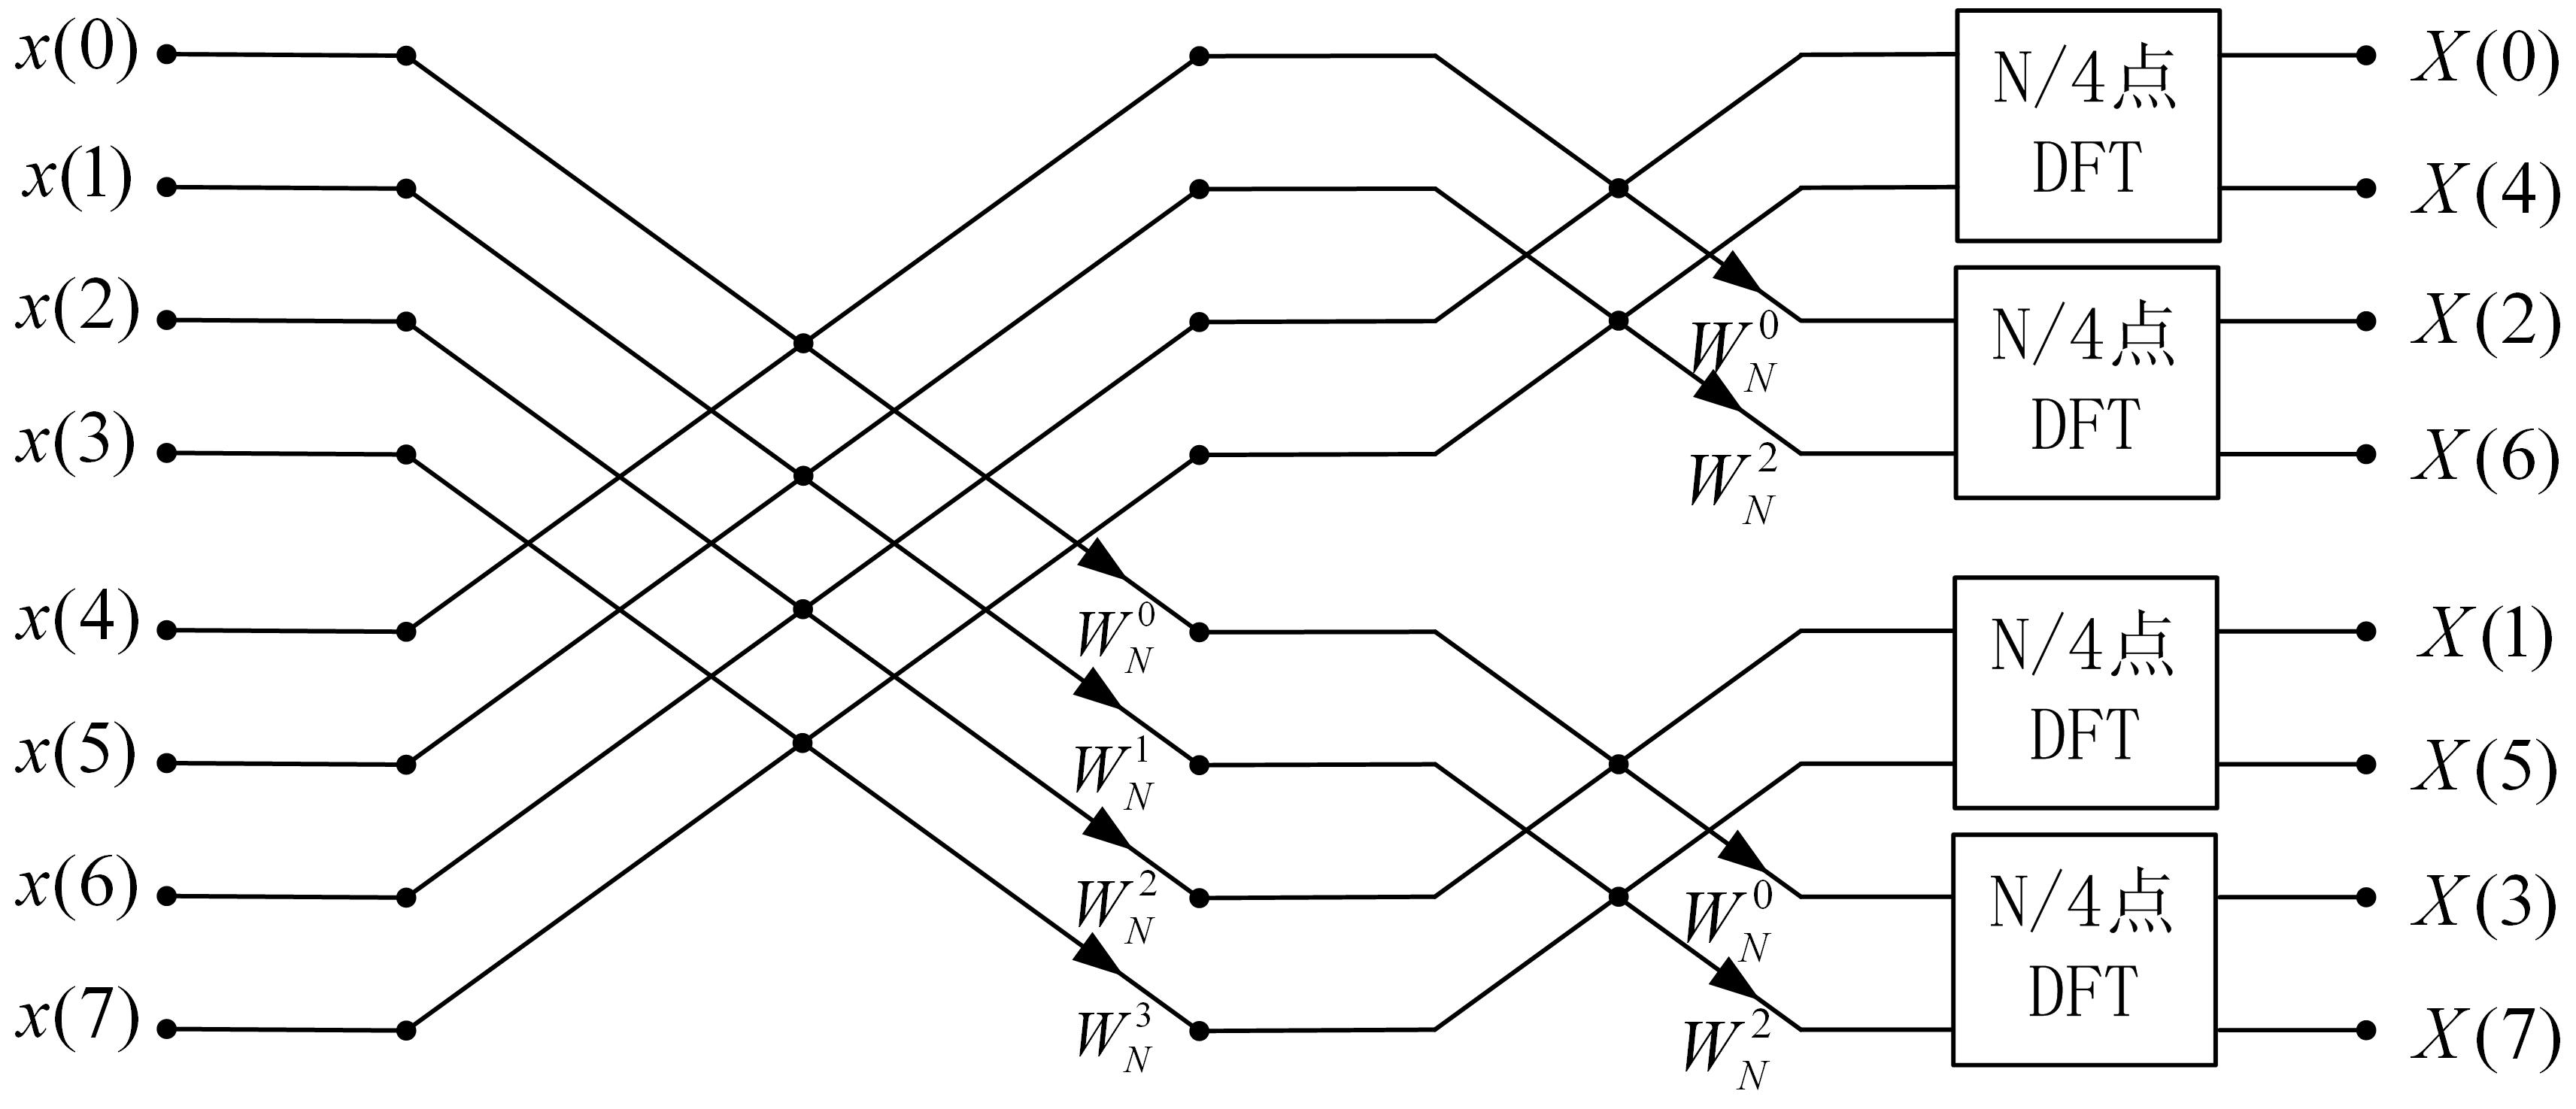
\includegraphics[width=0.99\textwidth]{dif8dftsecond.jpg}
  %\caption{8点DIF-DFT一次时域分解运算流图}
  %\label{}
\end{figure}
\end{frame}


\begin{frame}\frametitle{8点DIF-DFT三次时域分解运算流图}%[allowframebreaks]
\begin{figure}[h]
  \centering
  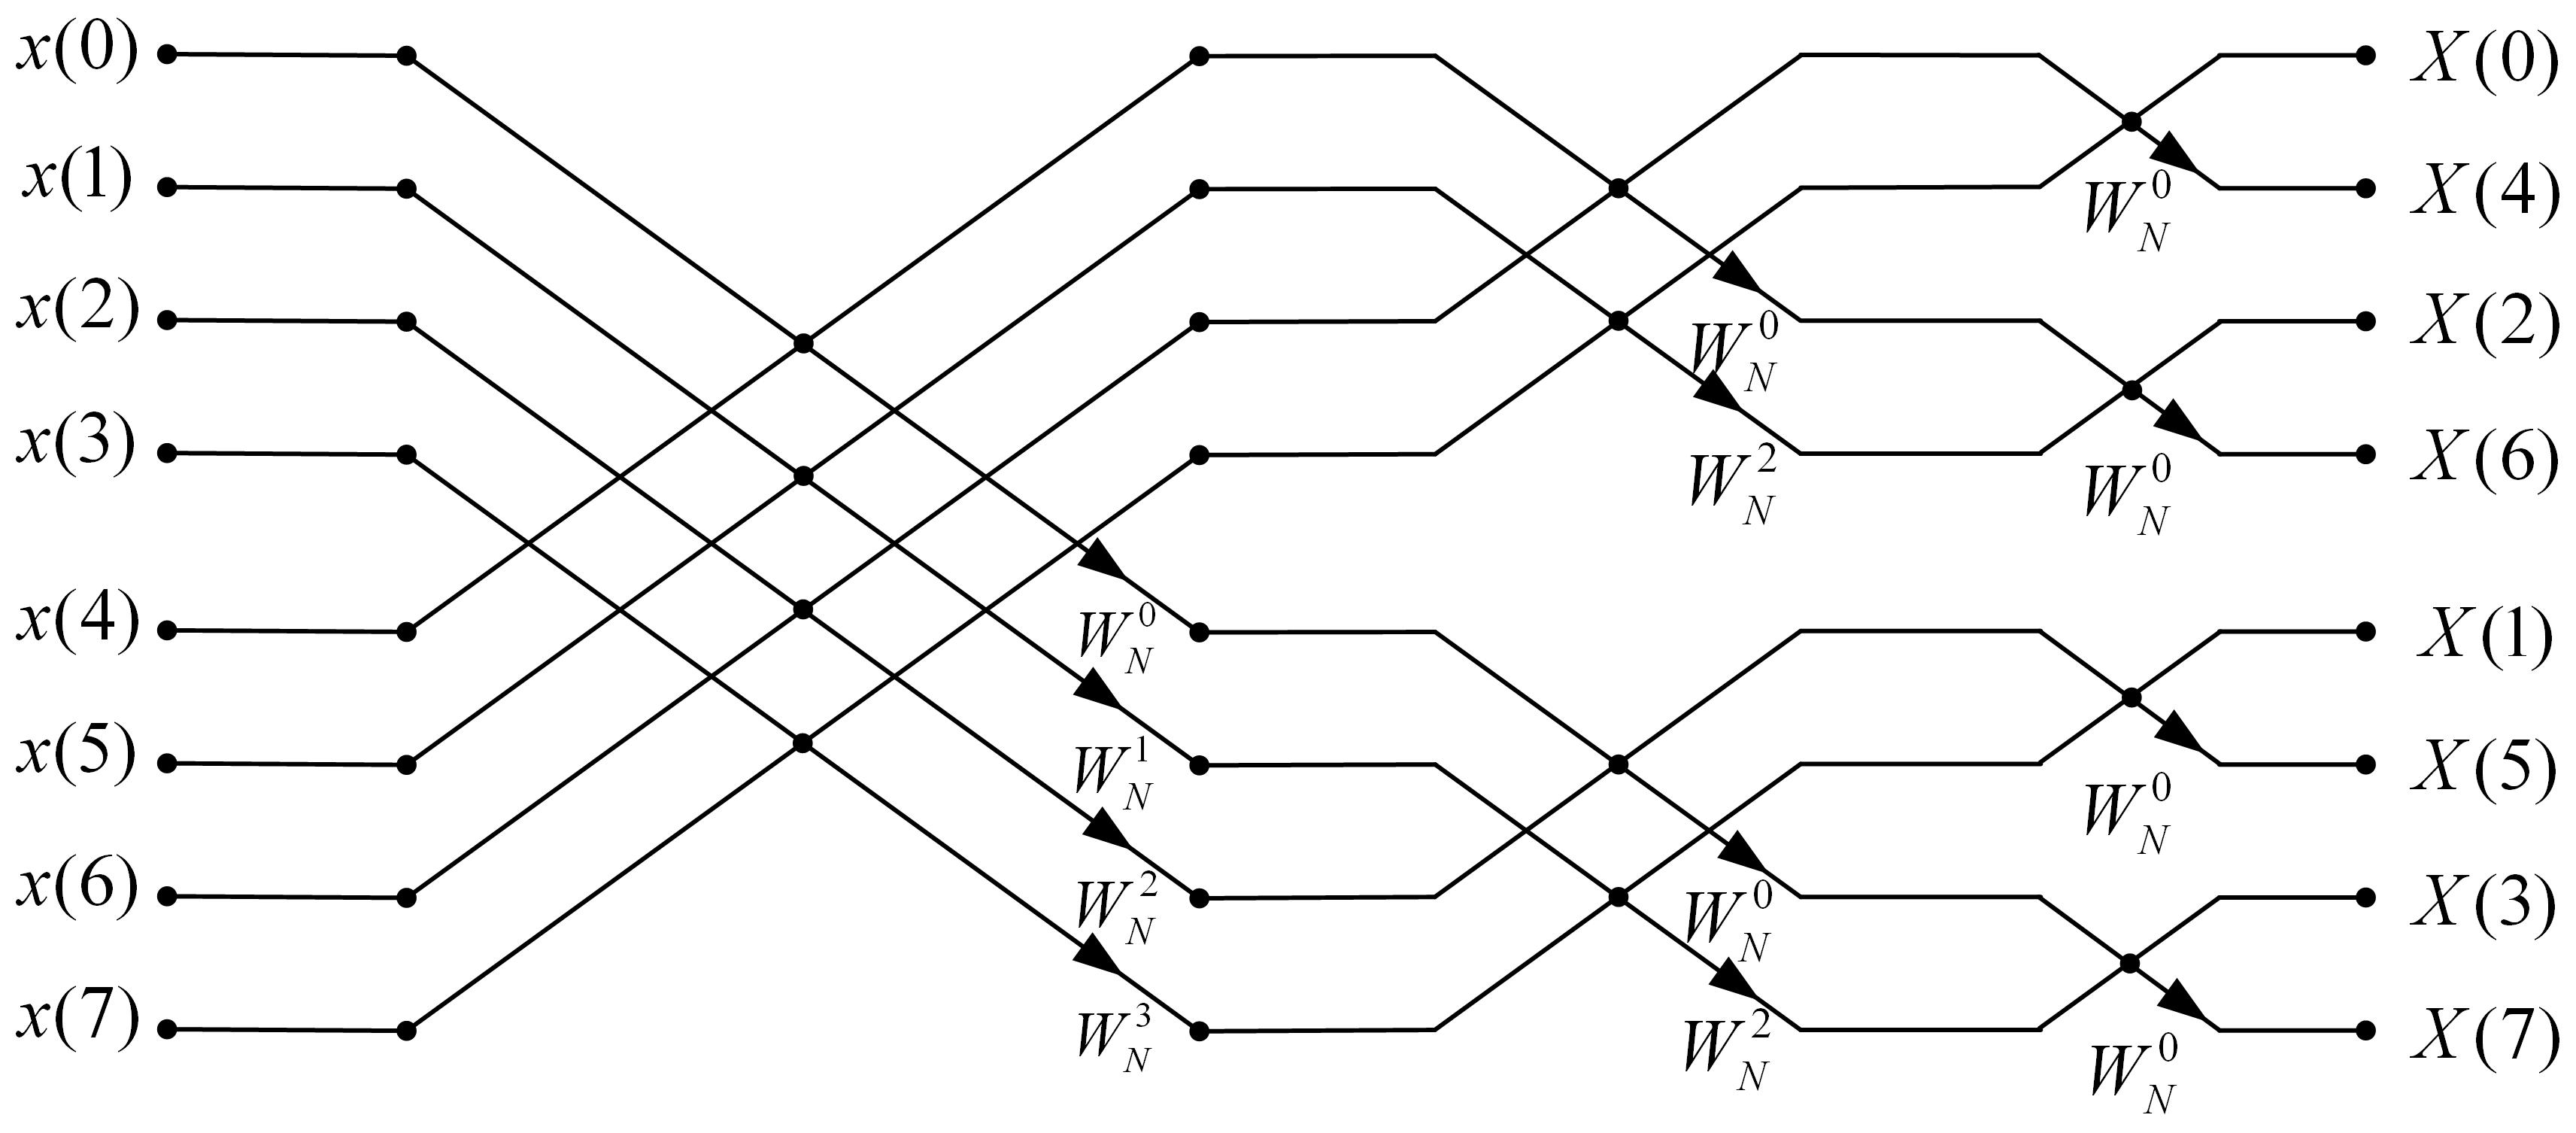
\includegraphics[width=0.99\textwidth]{dif8dftthird.jpg}
  %\caption{8点DIF-DFT一次时域分解运算流图}
  %\label{}
\end{figure}
\end{frame}



\section{IDFT的快速算法}
\subsection{方法一}
\begin{frame}\frametitle{IDFT的快速算法}%[allowframebreaks]
$$
\left \{
\begin{aligned}
    X(k)&= DFT[x(n)]\quad  = \quad\sum_{n=0}^{N-1}x(n)W_{N}^{kn}, &\quad (0\leq k\leq N-1)\\
    x(n)&= IDFT[X(k)] =\frac{1}{N}\sum_{n=0}^{N-1}X(k)W_{N}^{-kn},&\quad (0\leq n\leq N-1)
\end{aligned}
\right.
$$

\begin{itemize}
  \item  方法一: \par

        将$X(k)$作为输入,$p\rightarrow -p$,最后的结果除以$N$。
\end{itemize}
\end{frame}

\subsection{方法二}
%%%%------------------------------------------------------------------------------------------------
\begin{frame}\frametitle{IDFT的快速算法}%[allowframebreaks]
\begin{itemize}
  \item 方法二: \par
        %$$x(n)= \frac{1}{N}\sum_{n=0}^{N-1}X(k)W_{N}^{-kn}$$
        \begin{equation}
        \begin{split}
        x(n)&= \frac{1}{N}\sum_{n=0}^{N-1}X(k)W_{N}^{-kn} \quad\quad\quad\quad\quad\quad\quad\quad\quad\\
            &= \frac{1}{N}\left[\sum_{n=0}^{N-1}X^*(k)W_{N}^{kn} \right]^*\\
            &= \frac{1}{N}\left[DFT[X^*(k)]\right]^*\\
        \end{split}
        \end{equation}
       % $$
%        x(n)= \frac{1}{N}\sum_{n=0}^{N-1}X(k)W_{N}^{-kn}
%            = \frac{1}{N}\left[\sum_{n=0}^{N-1}X^*(k)W_{N}^{kn} \right]^*
%            = \frac{1}{N}\left[DFT[X^*(k)]\right]^*
%        $$
        将$X(k)$取共轭,做$DFT$变换,再将结果取共轭,最后除以$N$。
\end{itemize}

\end{frame}



%%%%%%%%%%%%%%%%%%%%%%%%%%%%%%%%%%%%%%%%%%%%%%%%%%%%%%%%%%%%%%%%%%%%%%%%%%%%%%%%%%%%%%%%%%%%%%
\end{document}

